\documentclass[UTF8]{ctexart}
%\IEEEoverridecommandlockouts
% The preceding line is only needed to identify funding in the first footnote. If that is unneeded, please comment it out.
\usepackage[linesnumbered,ruled,vlined]{algorithm2e}
%\usepackage{mathptm}
%\usepackage{algorithm}
\usepackage[noend]{algpseudocode}
\usepackage{amsmath}
\usepackage{amssymb}
%\usepackage{bbold}
\usepackage[inline]{enumitem}
\usepackage{epsfig}
\usepackage{fancyvrb}
\usepackage{graphicx}
\usepackage{booktabs, tabularx}
\usepackage[flushleft]{threeparttable}
\usepackage{latexsym, color}
\usepackage{listings}
% \usepackage[tight,footnotesize]{subfigure}
\usepackage{tikz}
\usepackage{times}
\usepackage{url}
\usepackage[font=normalsize,labelfont=bf]{caption}
\usepackage{hyperref}
\usepackage{cleveref}
\usepackage{tabularx}
\usepackage{subcaption}
\usepackage{multirow}
\usepackage{cite}
% Jensen
% highlight citation
\hypersetup{
  colorlinks=true,
  linkcolor=blue,
  citecolor=blue,
  urlcolor=magenta
}

% GK
%% macros for algorithm, added by QX
\SetKwProg{Fn}{Function}{}{end}
\SetFuncSty{textsc}

%%% Added by GK: helper macros [[[
\newcommand\Algref[1]{Algorithm~\ref{alg:#1}}

\newcommand\Figref[1]{Figure~\ref{fig:#1}}
\newcommand\Tblref[1]{Table~\ref{tbl:#1}}
%%% ]]]

% Set enumerate style to 1, 1.1
\renewcommand{\labelenumi}{\arabic{enumi}.}
\renewcommand{\labelenumii}{\arabic{enumi}.\arabic{enumii}}

\lstset{ %
language=Python,                % choose the language of the code
basicstyle=\scriptsize,       % the size of the fonts that are used for the code
numbers=left,                   % where to put the line-numbers
numberstyle=\scriptsize,      % the size of the fonts that are used for the line-numbers
stepnumber=1,                   % the step between two line-numbers. If it is 1 each line will be numbered
numbersep=5pt,                  % how far the line-numbers are from the code
backgroundcolor=\color{white},  % choose the background color. You must add \usepackage{color}
showspaces=false,               % show spaces adding particular underscores
showstringspaces=false,         % underline spaces within strings
showtabs=false,                 % show tabs within strings adding particular underscores
frame=single,           % adds a frame around the code
tabsize=2,          % sets default tabsize to 2 spaces
captionpos=b,           % sets the caption-position to bottom
breaklines=true,        % sets automatic line breaking
breakatwhitespace=false,    % sets if automatic breaks should only happen at whitespace
escapeinside={\%*}{*)}          % if you want to add a comment within your code
}
%\usepackage{algorithmic}
%\usepackage{algorithm}
%\renewcommand{\algorithmicwhile}{\textbf{upon-event}}
%\renewcommand{\algorithmicend}{\textbf{end}}
%\renewcommand{\algorithmicdo}{\textbf{do}}
%\floatname{algorithm}{Procedure}
\pagestyle{plain}

\allowdisplaybreaks
\setlength{\textfloatsep}{2pt}
\setlength{\intextsep}{2pt}

\renewcommand{\baselinestretch}{1.01}

\newenvironment{senumerate}{\begin{enumerate}%
\addtolength{\itemsep}{-6pt}%
}{\end{enumerate}}

\newenvironment{sitemize}{\begin{itemize}%
\addtolength{\itemsep}{-6pt}%
}{\end{itemize}}

\long\def\comment#1{}
\newtheorem{theorem}{\textbf{Theorem}}
\newtheorem{lemma}{\textbf{Lemma}}
\newtheorem{definition}{\textbf{Definition}}
\newtheorem{proposition}{\textbf{Proposition}}
\newtheorem{problem}{\textbf{Problem}}
\newtheorem{observation}{\textbf{Observation}}

\usepackage{float}
\usepackage{xspace}
% \newcommand{\subcaption}[1]{\centerline{#1}\vspace{0.1in}}
\newcommand{\ie}{{\em i.e.}}
\newcommand{\eg}{{\em e.g.}}
\newcommand{\etal}{{\em et al.}}
\newcommand{\defas}{\stackrel{\scriptscriptstyle\triangle}{=}}
\newcommand{\pattr}{\ensuremath{\mathit{pattr}}}


%%%%%%%%%%%%%%%%%%%%% BNF
\newcommand{\rulesep}{\unskip\ \vrule\ }
\newcommand \bnfdef  {\mathrel{\color{blue}{::=}}}
\newcommand \bnfalt  {\mathrel{\color{blue}{|}}}

\newcommand \keyfont {\mathsf}
\newcommand \ONPKT {\keyfont{onPacket(pkt)}}
\newcommand \WHILE  {\keyfont{while}}
\newcommand \IF     {\keyfont{if}}
\newcommand \THEN     {\keyfont{then}}
\newcommand \SKIP   {\keyfont{skip}}
\newcommand \RETURN   {\keyfont{return}}
\newcommand \ADD   {\keyfont{add}}
\newcommand \CONTAINS   {\keyfont{contains}}
\newcommand \GET   {\keyfont{get}}
\newcommand \PUT   {\keyfont{put}}
\newcommand \GLOBAL   {\keyfont{global}}
\newcommand \forl   {\keyfont{for}}
\newcommand \while[2]   {\WHILE\ {#1}\ {#2}}
\newcommand \ifelse[3]  {\IF\ {#1}:{#2}\ \THEN:{#3}}
\newcommand \return[1]   { \RETURN\ {#1}}
\newcommand \CYCLIC  {\keyfont{loop}}
\newcommand \cyclic[1]   { \CYCLIC\ {#1}}

\newcommand \JUMP  {\keyfont{jump}}
\newcommand \CJUMP  {\keyfont{cjump}}
\newcommand \LBL  {\keyfont{label}}

\newcommand \jump[1]   { \JUMP\ {#1}}
\newcommand \cjump[3]   { \CJUMP\ {#1}\ {#2}\ {#3}}
\newcommand \lbl[1]   { \LBL\ {#1}}

\newcommand \tx {\mathtt{x}}
\newcommand \ty {\mathtt{y}}
\newcommand \tz {\mathtt{z}}
\newcommand \tg {\mathtt{g}}

\setlength{\textfloatsep}{2pt}
\setlength{\intextsep}{2pt}



%Dynamic Stateful Datapath Configuration
\newcommand{\concept}{{Dandelion}}

\newcommand{\flowBGP}{SFP-1}
\newcommand{\SFP}{SFP}
\newcommand{\odl}{OpenDaylight}
\newcommand{\floodlight}{Floodlight}
\newcommand{\RSA}{ReSA}
\newcommand{\ODI}{ODI}
\newcommand{\ODIMAX}{{\sc MaxODI}}
\newcommand{\RIBComp}{{\sc SeqRIB}}
\newcommand{\system}{{\sc DSDC}}


\newcommand\Snoopy{{SN{\small OO}P{\small Y}}}
\newcommand{\onpacket}{$\mathtt{onPacket}$}


%\newcommand{\yry}[1]{{\small {\bf [yry: #1]}}}
\newcommand{\dkt}[1]{\textcolor{red}{DKT: #1}}
\newcommand{\todo}[1]{\textcolor{red}{TODO: #1}}
\newcommand{\para}[1]{\noindent {\bf #1}}%remove \smallskip
\newcommand{\yry}[1]{\textcolor{red}{[yry: #1]}}
\newcommand{\jensen}[1]{\textcolor{red}{[jensen: #1]}}
\newcommand{\jace}[1]{\textcolor{red}{[jace: #1]}}
\newcommand{\q}[1]{\textcolor{red}{[qiao: #1]}}
\newcommand{\old}[1]{\textcolor{red}{[oldtext: #1]}}
\newcommand{\tony}[1]{\textcolor{red}{[tony: #1]}}

\newcommand{\codeword}[1]{\texttt{\small{#1}}}



%\newcommand{\al}[1]{\addtocounter{linenum}{1}\arabic{linenum}\'#1\\}
\newcommand{\al}[1]{\'#1\\}
\newcommand{\all}[1]{\addtocounter{linenum}{1}\arabic{linenum}\'#1}
\newcommand{\av}[1]{\textit{#1}}
\newcommand{\aproc}[2]{\textsc{#1}\((#2)\)}
\newcommand{\kw}[1]{\textbf{#1}}
\newcommand{\msg}[2]{$\langle$\textsl{#1};$#2 \rangle$}

\newcommand{\tabincell}[2]{\begin{tabular}{@{}#1@{}}#2\end{tabular}}

\newcommand{\Tabs}{
  xx\= xx\= xx\= xx\= xx\= xx\= xx\= xx\=xx\= xx\= xx\= xx\=\kill}

\newlength{\figurewidthA} % 1 figure in a row (1 column)
\setlength{\figurewidthA}{0.6\columnwidth}

\newlength{\figurewidthB} % 3 figures in a row (2 columns)
\setlength{\figurewidthB}{0.5\columnwidth}

\newlength{\figurewidthC} % adjust sizes of figures to save space
\setlength{\figurewidthC}{0.55\columnwidth}

\newlength{\algFrameSize} %
\setlength{\algFrameSize}{3.3in}

\iffalse
%%%%%%%%% To format algorithm %%%%%%%%%%%%%%%%%%%%%%%%%%%
\newcounter{linenum}
\newenvironment{algorithm}[2]{\setcounter{linenum}{0}\begin{tabbing}\textsc{#1}\((#2)\)\\
\makebox[0.2in]{}\=\+\kill}{\end{tabbing}}
\newenvironment{protocol}{\setcounter{linenum}{0}\begin{tabbing}\makebox[0.05in]{}\=\+\kill}{\end{tabbing}}
\newenvironment{note}%
  {\trivlist \item[\hskip \labelsep {\em Note\/}]}{\endtrivlist}
\newenvironment{remark}%
  {\trivlist \item[\hskip \labelsep {\em Remark\/}]}{\endtrivlist}
\fi





\newenvironment{program}[3]{
  \begin{figure}[hbtp]
    \begin{center}
    \fbox{
      {\small % yry
      \begin{minipage}{\textwidth}
      \begin{tabbing}
      \Tabs
      #3
      \end{tabbing}
      \vspace{-0.25in}
      \end{minipage}
      } % yry
    \vspace{-0.15in}
    }
    \end{center}
    \vspace{-0.2in}
    \caption{\label{#1} #2}
    \vspace{-0.1in}
  \end{figure}}{}

\newcommand{\squishlist}{
   \begin{list}{$\bullet$}
    { \setlength{\itemsep}{0pt}      \setlength{\parsep}{3pt}
      \setlength{\topsep}{3pt}       \setlength{\partopsep}{0pt}
      \setlength{\leftmargin}{3.5mm} \setlength{\labelwidth}{1em}
      \setlength{\labelsep}{0.5em} } }

\newcommand{\squishlisttwo}{
   \begin{list}{$\bullet$}
    { \setlength{\itemsep}{0pt}    \setlength{\parsep}{0pt}
      \setlength{\topsep}{0pt}     \setlength{\partopsep}{0pt}
      \setlength{\leftmargin}{2em} \setlength{\labelwidth}{1.5em}
      \setlength{\labelsep}{0.5em} } }

\newcommand{\squishend}{
    \end{list}  }
\newenvironment{squished}{\squishlist}{\squishend}

\newenvironment{icompact}{
  \begin{list}{$\bullet$}{
    \parsep 0pt plus 1pt
    \partopsep 0pt plus 1pt
    \topsep 2pt plus 2pt minus 1pt
    \itemsep 0pt plus 0pt
%    \itemsep 0pt plus 1pt
    \parskip 0pt plus 0pt
%    \parskip 0pt plus 2pt
    \leftmargin 0.2in}
%    \leftmargin 0.3in}
       \raggedright}
  {\normalsize\end{list}}

\newcommand{\parab}[1]{\vspace*{0.5ex}\noindent\textbf{#1}}
\newcommand{\parae}[1]{\vspace*{0.5ex}\noindent\emph{#1}}
\newcommand{\parabe}[1]{\vspace*{0.5ex}\noindent\textbf{\emph{#1}}}

%%%%%%%% to calculate the time %%%%%%%%%%%%%%%%%%%%%%%%%%%%
\newcount\hour \newcount\minute
\hour=\time  \divide \hour by 60
\minute=\time
\loop \ifnum \minute > 59 \advance \minute by -60 \repeat
\def\drafttime{\ifnum \hour<13 \number\hour:%
                      \ifnum \minute<10 0\fi
                      \number\minute
                      \ifnum \hour<12 \ AM\else \ PM\fi
         \else \advance \hour by -12 \number\hour:%
                      \ifnum \minute<10 0\fi
                      \number\minute \ PM\fi}
\def\timestamp{\today \ \drafttime}

%added by SX: switch-case,assert statements for algorithmic
%\algnewcommand\algorithmicswitch{\textbf{switch}}
%\algnewcommand\algorithmiccase{\textbf{case}}
%\algnewcommand\algorithmicdefault{\textbf{default}}
%\algnewcommand\algorithmicassert{\texttt{assert}}
%\algnewcommand\Assert[1]{\State \algorithmicassert(#1)}%
%\algdef{SE}[CASE]{Case}{EndCase}[1]{\algorithmiccase\ #1:}{\algorithmicend\ \algorithmiccase}%
%\algdef{SE}[DEFAULT]{Default}{EndDefault}{\algorithmicdefault:}{\algorithmicend\ \algorithmicdefault}%
%\algtext*{EndCase}%
%\algtext*{EndDefault}%
%\newcommand{\Switch}[1]{\State \textbf{switch} $($#1$)$ \textbf{do}}
%\newcommand{\EndSwitch}{\State \textbf{end switch}}

%\algnewcommand\algorithmicforeach{\textbf{for each}}
%\algdef{S}[FOR]{ForEach}[1]{\algorithmicforeach\ #1\ \algorithmicdo}


\usepackage{setspace}
\begin{document}

\title{\huge \concept{}: A Novel, High-Level Programming System for Software
Defined Coalitions with Local State Sharing}
%Toward High-Level Efficient Programming

\author{ 
	Xin Wang$^{\dagger}$,
	Qiao Xiang$^{\dagger}$,
	Jeremy Tucker$^{\ddagger}$,
	Vinod Mishra$^{*}$,
	Y. Richard Yang$^{\dagger}$,\\ 
%	$^{\dagger}$Tongji University, 
	$^{\dagger}$Yale University,
	$^{\ddagger}$U.K. Defence Science and Technology Laboratory, 
	$^{*}$U.S. Army Research Labs,\\
%	13xinwang@tongji.edu.cn, 
	\{xin.wang, qiao.xiang, yry\}@cs.yale.edu,
	jtucker@mail.dstl.gov.uk, 
	vinod.k.mishra.civ@mail.mil 
}

\maketitle

\begin{abstract}
%\cleet{Note: authors placeholder}
%\cleet{Abstract placeholder}
High-level programming and programmable data paths are two key capabilities of software-defined networking (SDN). A fundamental problem linking these two capabilities is whether a given high-level SDN program can be realized onto a given low-level SDN datapath structure. Considering all high-level programs that can be realized onto a given datapath as the programming capacity of the datapath, we refer to this problem as the {\em SDN datapath programming capacity problem}. In this paper, we conduct the first study on the SDN datapath programming capacity problem, in the general setting of {\em high-level, datapath oblivious, algorithmic SDN programs} and state-of-art {\em multi-table SDN datapath pipelines}. In particular, considering datapath-oblivious SDN programs as computations and datapath pipelines as computation capabilities, we introduce a novel framework called {\em SDN characterization functions}, to map both SDN programs and datapaths into a  unifying space, deriving the first rigorous result on SDN datapath programming capacity. We not only prove our results but also conduct realistic evaluations to demonstrate the tightness of our analysis. 
%\yry{Need a word on tightness}

% Despite the emergence of multi-table pipelining as a key feature of next-generation SDN datapath models, there is no existing work addresses the substantial challenge of utilizing pipelines automatically for a datapath oblivious program.
% This is the first work that systematically studies the complex structure of general SDN datapath pipelines and investigate how to embed a high-level datapath oblivious SDN program into the pipelines. We develop a novel Capacity Theorem, by which we can verify whether an SDN program can be embedded into the pipelines based on two vectors, Equivalence Class vector and Capacity vector, extracted from SDN programs and the pipelines respectively. We also design two novel algorithms, ComputeEV for programs and ComputeCVForMP for pipelines, to extract two vectors. By the two vectors and the proposed Capacity Theorem, we can express the requirements of programs and the abilities pf pipelines without including the complex inner structures.
\end{abstract}







\section{Introduction}\label{sec:introduction}
%\cleet{Introduction placeholder text}
A major research direction of SDN is programmable, efficient datapaths (\eg, OF1.3~\cite{openflow13}, OF-DPA~\cite{OF-DPA}, P4~\cite{P4}). Only by being programmable can a given SDN datapath support diverse, ever evolving application scenarios. At the same time, it is crucial that datapaths be efficient, to be able to satisfy demanding requirements such as achieving high throughput and being cost effective. In the last few years, multi-table pipelines have emerged as a key structure of SDN datapaths (\eg, Domino~\cite{Domino}, Forwarding Metamorphosis~\cite{bosshart2013forwarding}). 

%A problem of efficient datapaths, however, is that they can be low level to program.

One problem of efficient datapaths, however, is that they must often be programmed at an inefficiently low level. For example, TCAM, which is essential to achieve high-throughput, does not support logical negation. Hence, a second major research direction of SDN is high-level, datapath path-oblivious programming, to provide abstractions to hide low-level datapath programming. To this end, in the last few years multiple high-level SDN programming models have emerged (\eg, Frenetic~\cite{frenetic}, Maple~\cite{maple}).

As both directions progress, a basic problem emerges: whether a given high-level program can be realized on a given low-level datapath. A good understanding of this problem can benefit both the design of high-level SDN programming and the design of datapaths. Given a fixed datapath (\eg, a fixed pipeline architecture such as OF-DPA), the vendor of the datapath can provide guidelines on the high-level programs that can be realized. Given a set of high-level programs to be supported, one could use this understanding to design the most compact datapath supporting these programs. Even for reconfigurable datapaths (\eg, P4), as reconfiguration can be expensive and time consuming, one can use this understanding to guide the design of a more robust datapath. Considering all high-level programs that can be realized onto a given programmable datapath as the capacity of the datapath, we define the basic problem as the {\em SDN datapath programming capacity problem}.

%\begin{figure}[h!]
%    \centering
%    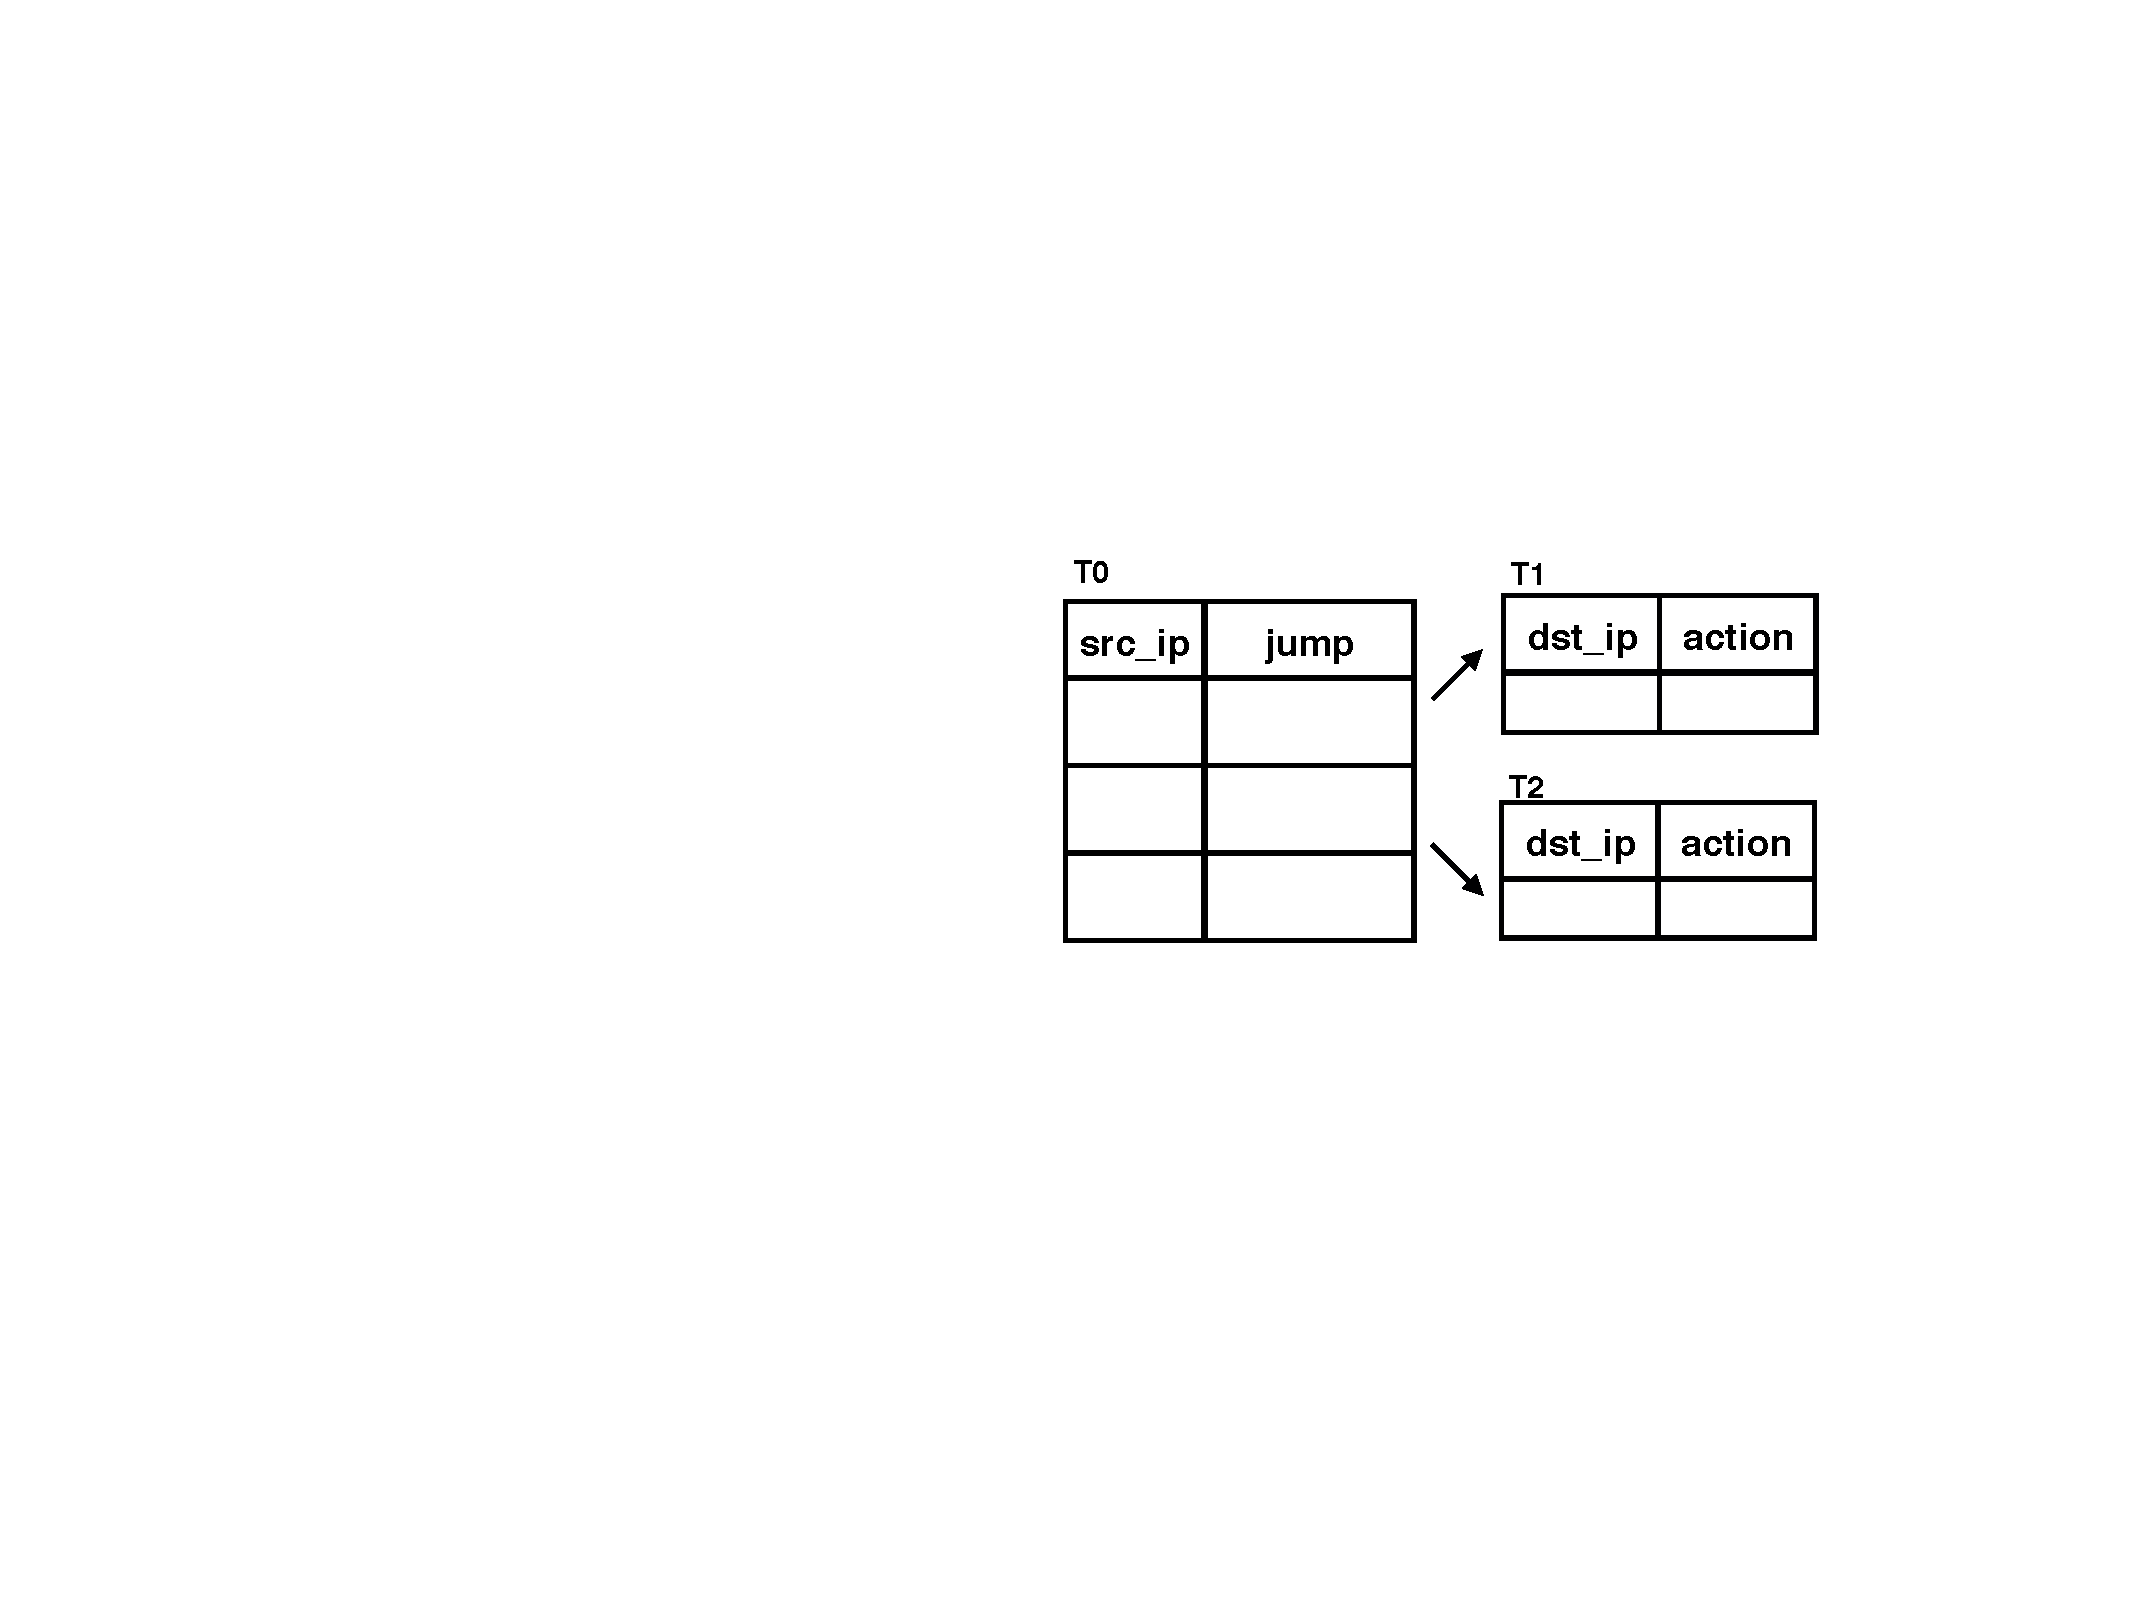
\includegraphics[width=3.25in]{figures/fig1-update.pdf}
%%    \vspace{-0.3in}
%    \caption{Example datapath.}
%    \label{fig:fig1-update}
%\end{figure}

% Solving the datapath programming capacity problem, however, is not trivial. Consider a high-level program \texttt{onPkt} shown in Sec.~\ref{sec:model-and-main-results}. The if statements in the program make the structure complex and the flexibility of table design makes the formalization of program hard. It is not desirable to make much restriction on programmers when they are writing high-level programs. Also, from the other side, consider a pipeline \texttt{swP} shown in Sec.~\ref{sec:model-and-main-results} Though the pipeline \texttt{swP} also defines a set tables, the layout might be different with the program \texttt{onPkt}, which including the pipeline structure and table matching fields. For example, the program \texttt{onPkt} requires a table matching both $dstAddr$ and $dstPort$ which does not exist in the pipeline \texttt{swP}. It is not obvious to see whether the program can be realized on the pipeline. 




%Fig.~\ref{fig:fig1-update}, which shows a simple datapath, named Example-DP, which consists of two-tables forming a pipeline. 
%Consider two simple high-level SDN programs [revise]. An interested reader can try to verify that the first program can be realized by Example-DP, but the second cannot. 
%{\small
%\begin{verbatim}
%// Program: L3-Route
%
%   onPacket(p):
%1.   s = p.srcIP
%2.   d = p.dstIP
%3.   if (s == "10.0.0.1"):
%4.     egress = myPolicyOne(d)
%5.   else
%6.     egress = myPolicyTwo(d)
%8.   return egress
%\end{verbatim}
%}
%
%{\small
%\begin{verbatim}
%// Program: L3-Route-Changed
%...
%4.   if (s == "10.0.0.1"):
%5.     egress = myPolicyOne(d)
%6.   else if (s == "10.0.0.2"):
%7.     egress = my PolicyThree(d)
%...
%\end{verbatim}
%}

%Consider a high-level program \texttt{onPkt} shown in Sec.~\ref{sec:model-and-main-results}. The if statements in the program make the structure complex and the flexibility of table design makes the formalization of program hard. It is not desirable to make much restriction on programmers when they are writing high-level programs. Also, from the other side, consider a pipeline \texttt{swP} shown in Sec.~\ref{sec:model-and-main-results} Though the pipeline \texttt{swP} also defines a set tables, the layout might be different with the program \texttt{onPkt}, which including the pipeline structure and table matching fields. For example, the program \texttt{onPkt} requires a table matching both $dstAddr$ and $dstPort$ which does not exist in the pipeline \texttt{swP}. It is not obvious to see whether the program can be realized on the pipeline. 



Solving the datapath capacity problem, however, is not trivial. 
Consider a simple datapath, named Simple-DP, shown in Fig.~\ref{fig:fig1-update}. It is among the simplest datapaths, consisting of three tables forming a pipeline, where the first table (\texttt{t1}) matches on source IP and may jump to one of the two following tables, which both match on destination IP.
\begin{figure}[h!]
    \centering
    \vspace{-0.1in}
    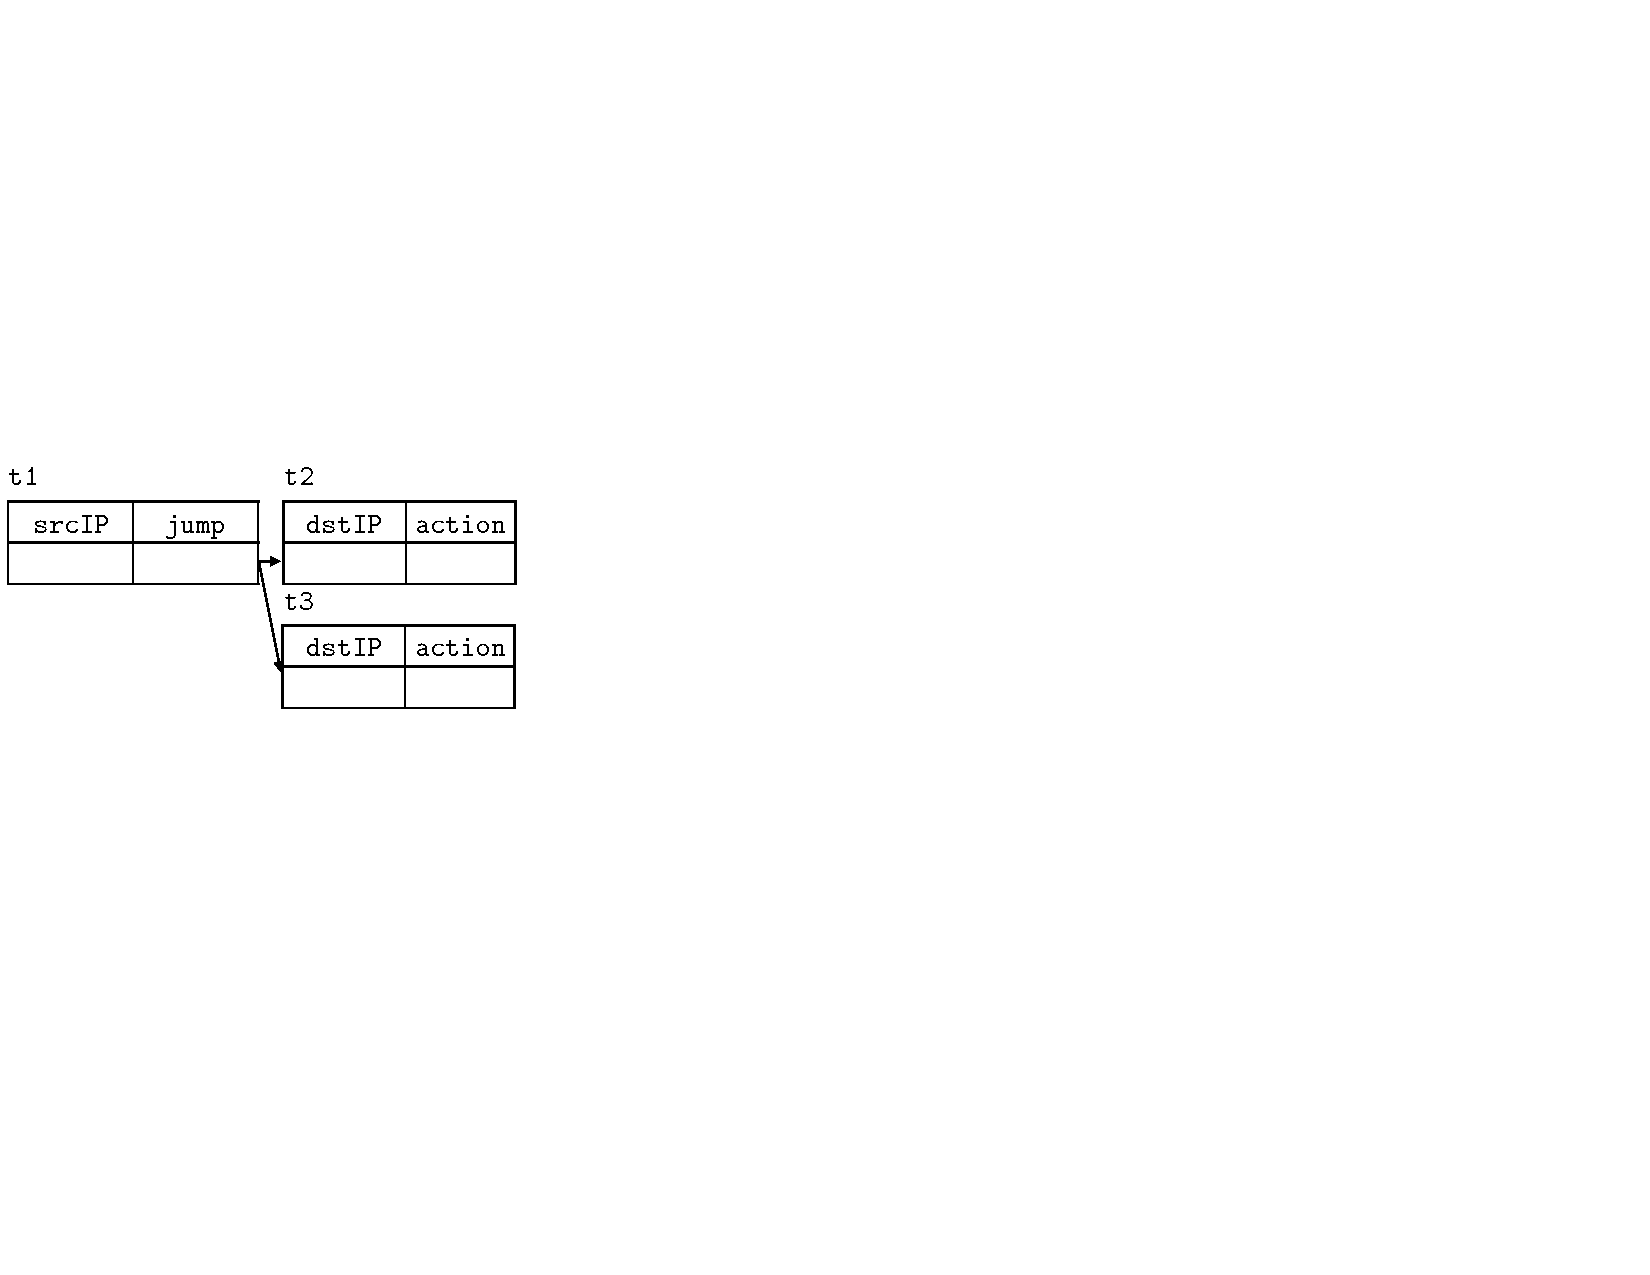
\includegraphics[scale = 0.7]{figures/figure1.pdf}
    \vspace{-0.1in}
    \caption{A simple example datapath: Simple-DP.}
    \vspace{-0.1in}
    \label{fig:fig1-update}
\end{figure}

Consider two simple high-level SDN programs below, both specified in the algorithmic, event-driven programming style to handle packet misses; see Sec. II for more details on the programming model. An interested reader can try to verify that the first program can be realized by Simple-DP, but the second cannot. 
{\small
\begin{verbatim}
//  Routing Function: secureL3Route
L0: secureL3Route(Addr srcIP, Addr dstIP):
L1:   if srcIP == 10.0.0.1:
L2:     return Forward(port=shortestPath(dstIP))
L3:   else:
L4:     return Drop();
\end{verbatim}
}

{\small
\begin{verbatim}
//  Program: twoHostL3Route
L0: def twoHostL3Route(Addr srcIP, Addr dstIP):
L1:   if srcIP == 10.0.0.1:
L2:     return Forward(port=shortestPath(dstIP)) 
L3:   elif srcIP == 10.0.0.2:
L4:     return Forward(port=securePath(dstIP))
L5:   else:
L6:     return Drop();
\end{verbatim}}

Although the preceding datapath and high-level programs are among the simplest, they may already appear to be non-trivial for a reader to analyze. General datapath and high-level programs can be much more complex as multiple services need to be implemented and hence they can pose severe challenges in analysis. The goal of this paper is to develop the first systematic methodology to solve the SDN datapath programming capacity problem. 

The contributions of this paper can be summarized as follows. First, we  propose a unifying characteristic functional space to unify and extract the essence of programs and pipelines, removing complexities such as program structures and pipeline layouts. Second, we define a comparator in this functional space, which can be used to check whether a high-level program can be realized on a given pipeline.

The rest of the paper is organized as follows. We define our model precisely in Sec.~\ref{sec:model-and-main-results}. The main results are given in Sec.~\ref{sec:main-results} and the proofs are shown in Sec.~\ref{sec:proofs}. Sec.~\ref{sec:evaluation} shows our evaluation results. Finally, related work is provided in Sec.~\ref{sec:related-work}.

\section{Related Work and Motivation}
\label{sec:motivation}

\para{Related work}: 
Some SDN/SDC datapaths are recently proposed to offload complex,
stateful operations on packets (\eg, counting, flow security inspection and
congestion control) from the control plane (\eg, a base station) to data plane
devices (\eg, mobile devices) to improve the performance of SDN
applications~\cite{arashloo2016snap, heorhiadi2016simplifying, soule2014merlin,
benet2018mp, katta2016hula, gember2012stratos, anwer2015programming,
monsanto2012compiler,
kohler2018p4cep, bianchi2014openstate, opensdc} under dynamic
tactical environments. 
In these designs, results of offloaded operations are
stored by each data plane device independently. We refer to them as
\textit{local states}.
SOL~\cite{heorhiadi2016simplifying} and Merlin~\cite{soule2014merlin}
tackle the placement and configuration of data plane devices by solving
constrained path computation problems.
  P4CEP~\cite{kohler2018p4cep} and OpenSDC~\cite{opensdc} focus on expanding the
capability of data plane devices from packet processing to event processing.
SNAP~\cite{arashloo2016snap} designs a high-level programming system that
translates a high-level program to the configuration of
stateful operations in data plane devices. Despite these substantial efforts
on stateful SDC datapath, one major, common limitation of these systems is that the local states of each data plane device are not
shared with others. As we will show shortly in the motivating example, this would lead to
substantial resource under-utilization in SDC networks, impairing the
performance of SDC applications. 

To allow local state sharing between data plane devices, DDP~\cite{ddp} designs
some  primitives for distributed datapath update. Hula~\cite{katta2016hula} and
MP-HULA~\cite{benet2018mp} also design probing mechanisms for data plane devices
running load balancing applications to update their local states.  However,
manually configuring such low-level primitives on an application-by-application
basis is time-consuming and error-prone.


%There are some related work (\eg, \cite{arashloo2016snap},
%\cite{heorhiadi2016simplifying}, \cite{soule2014merlin}, \cite{benet2018mp},
%\cite{katta2016hula}, \cite{gember2012stratos}, \cite{anwer2015programming},
%\cite{hinrichs2009practical}, \cite{monsanto2012compiler},
%\cite{kohler2018p4cep}, \cite{mcclurg2016event}) for the offloading problem.




%But it does not consider sharing local
%state among switches. 



\begin{figure}[!htbp]
%\vspace{-2mm}
\centering
\begin{subfigure}{0.8\linewidth}
      \centering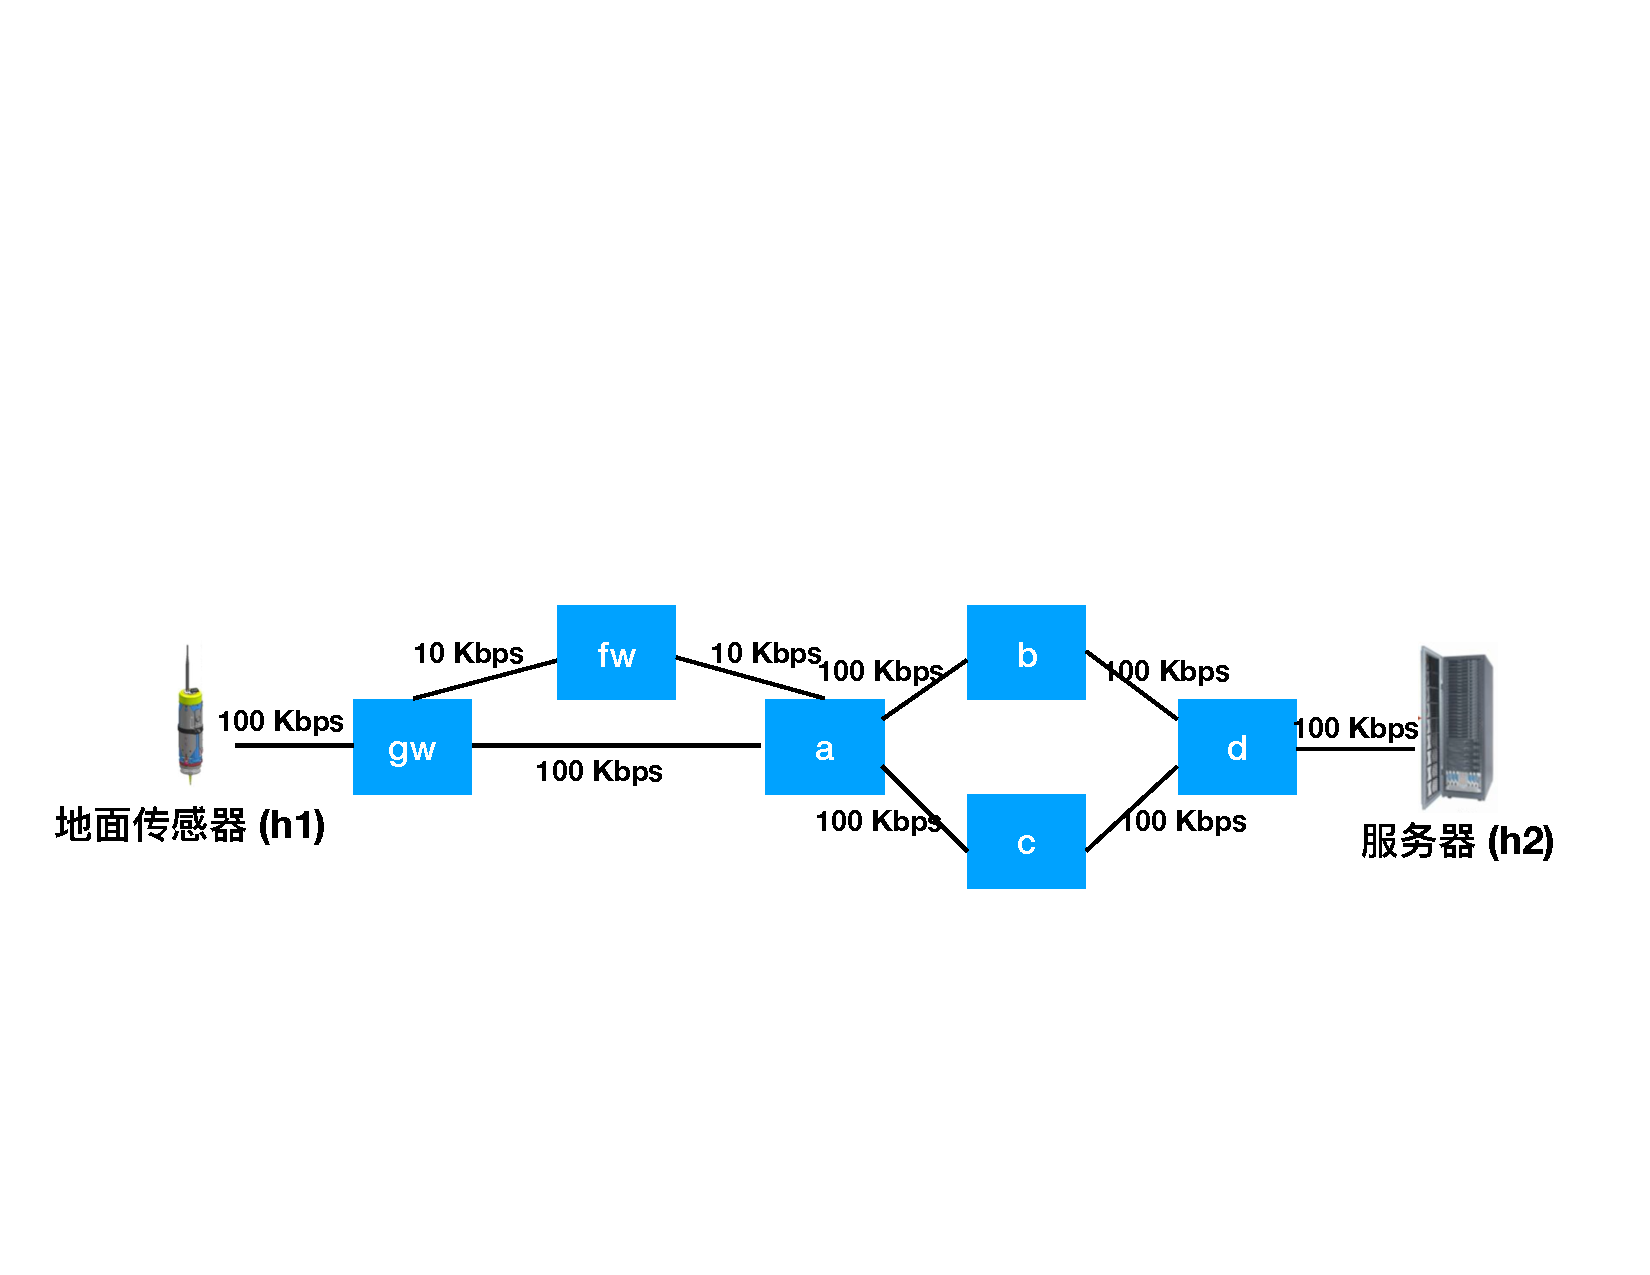
\includegraphics[width=\linewidth]{figures/ss-122.pdf}
      \caption{\label{fig:fw-topo} \small The network topology.}
\end{subfigure}
\hspace{0.03\linewidth}
\begin{subfigure}{0.8\linewidth}
      \centering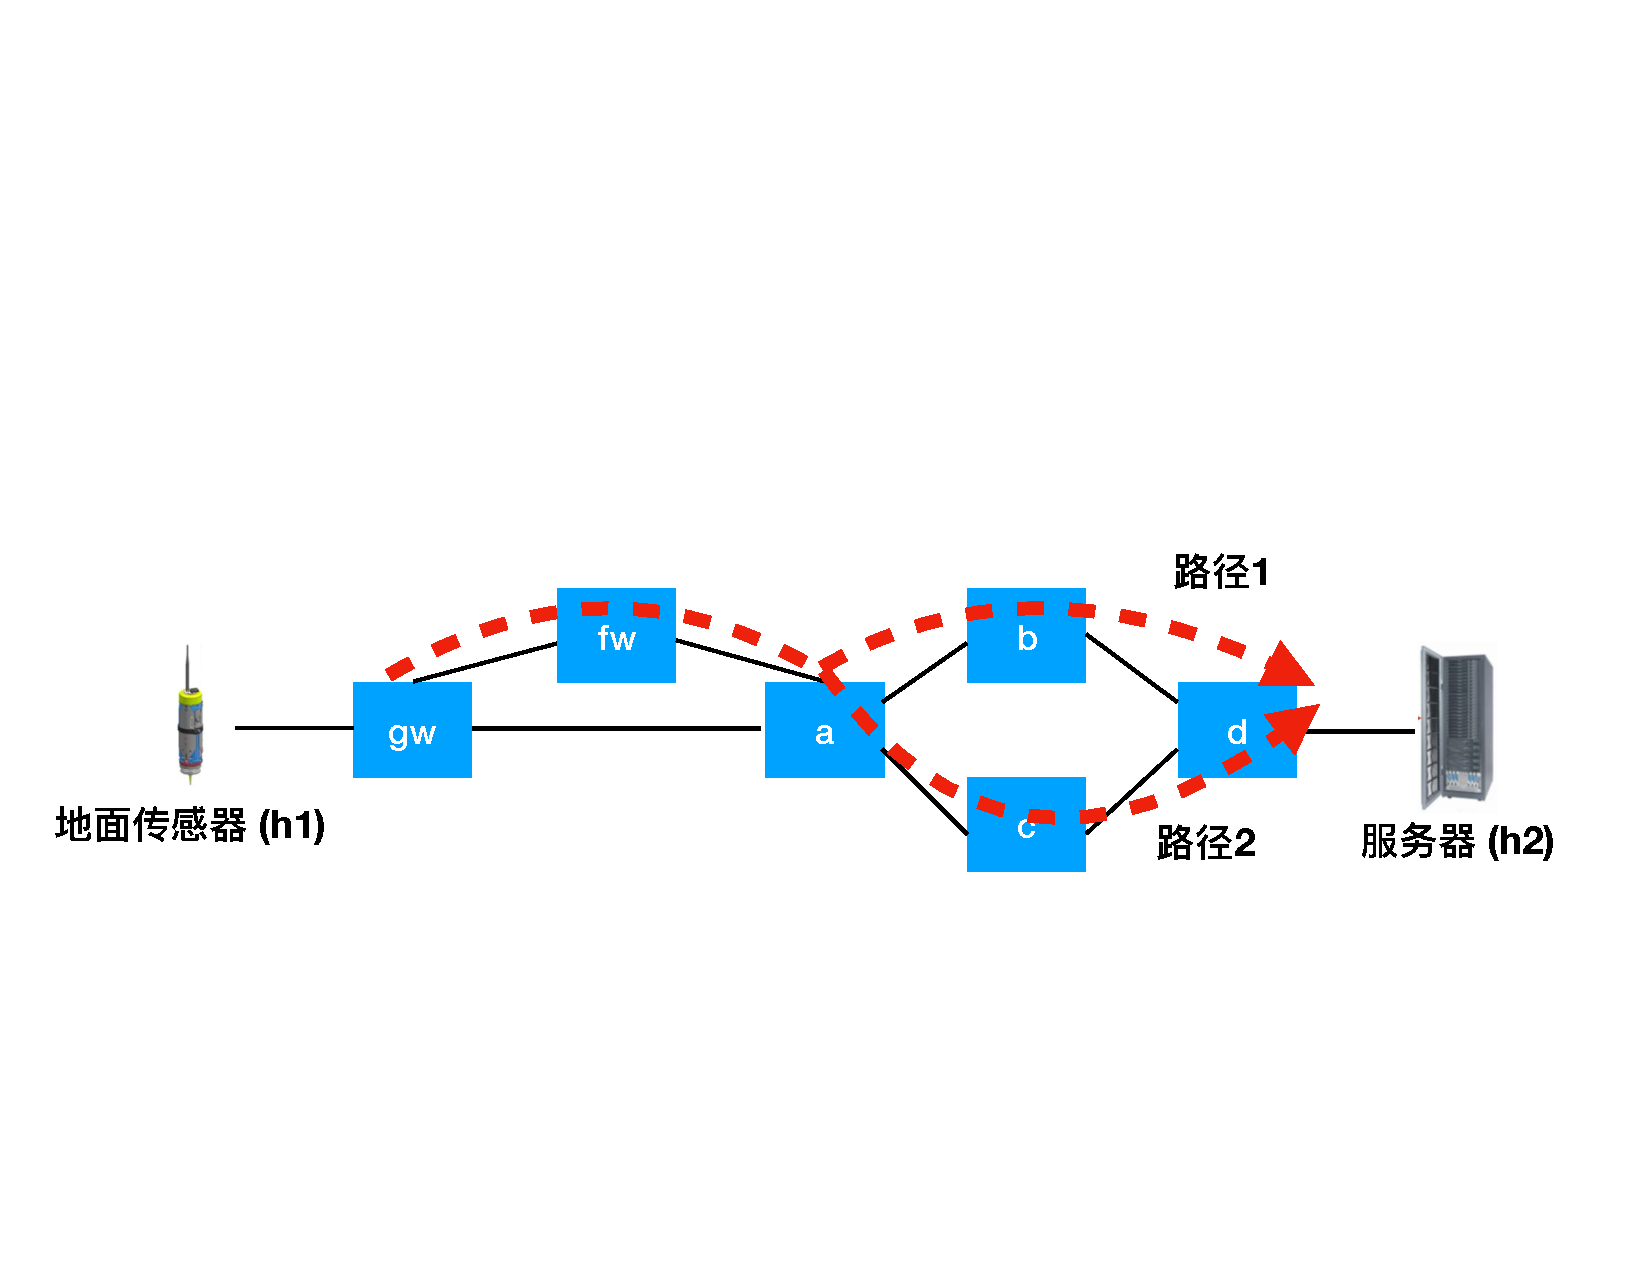
\includegraphics[width=\linewidth]{figures/ss-123.pdf}
      \caption{\label{fig:existing-result} \small The data plane configuration
	without local state sharing.}
\end{subfigure}
%\begin{subfigure}{0.8\linewidth}
%      \centering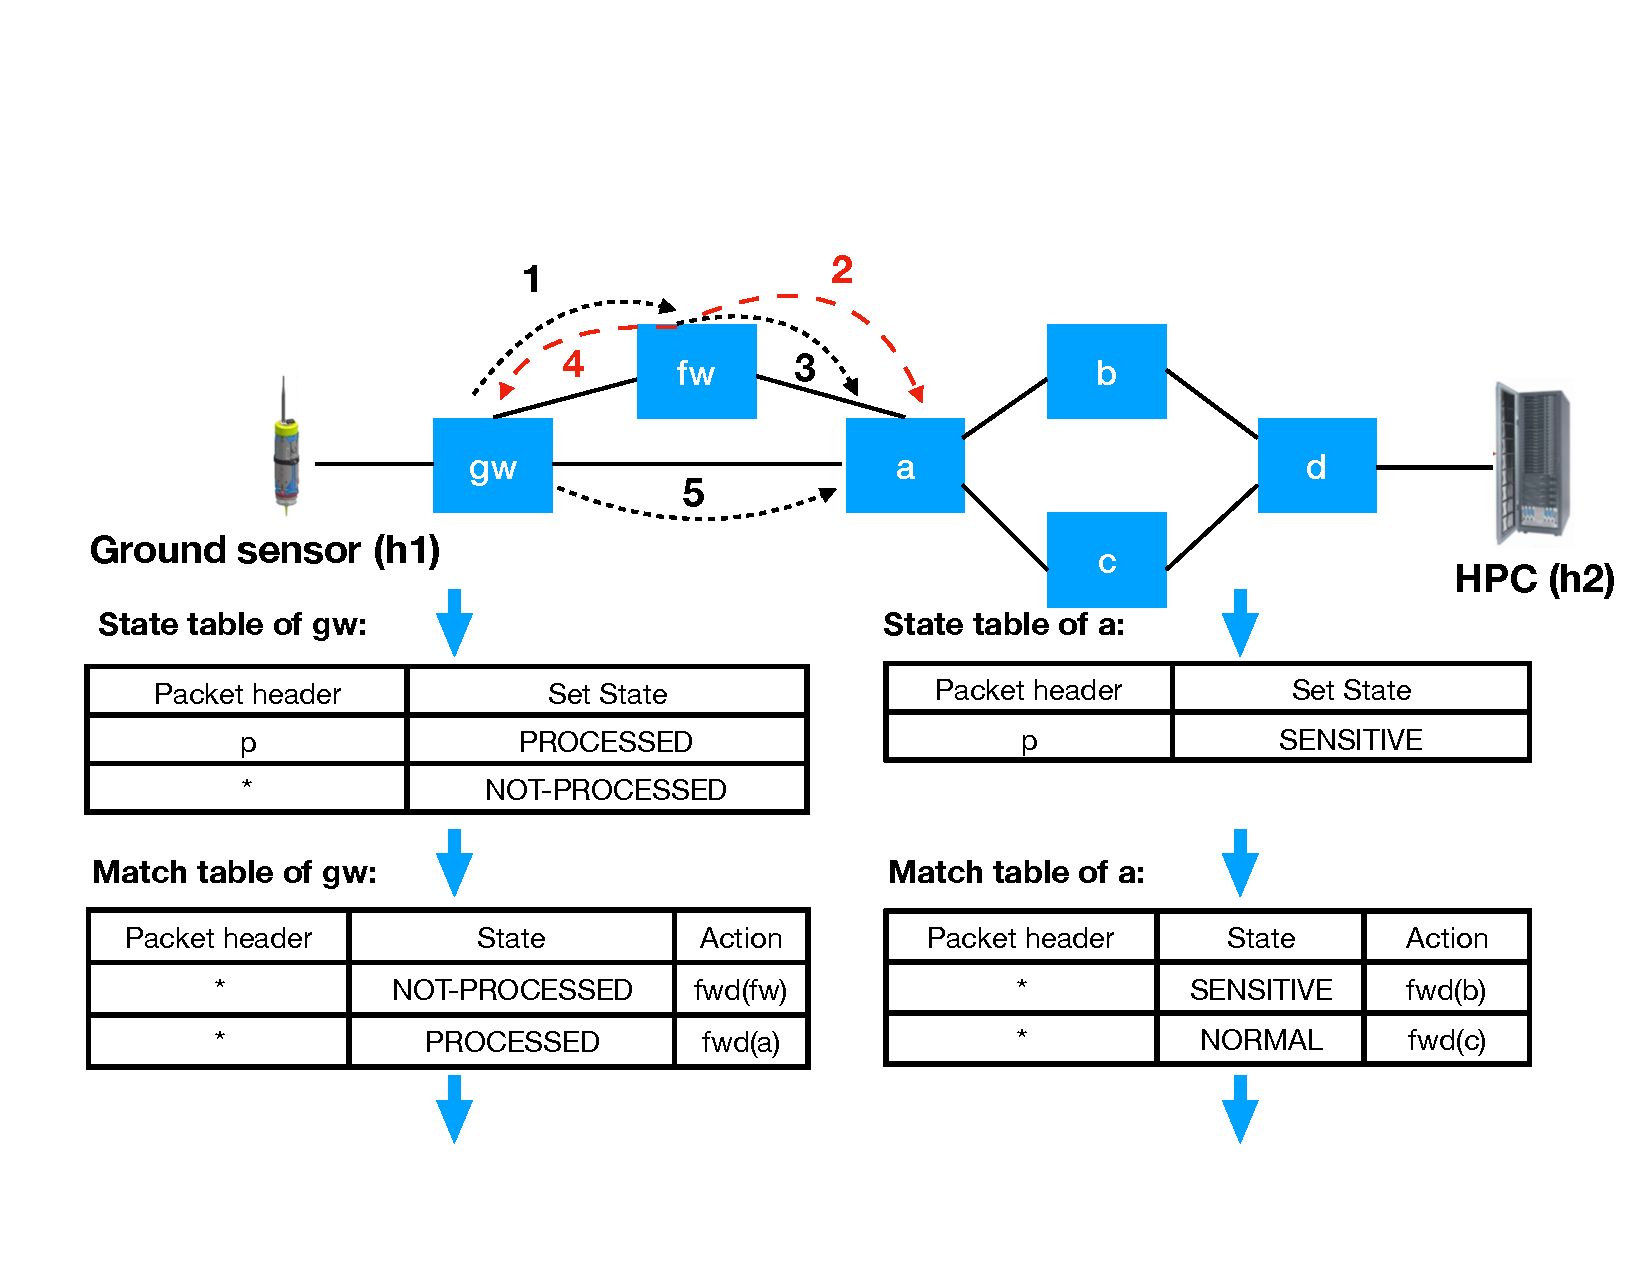
\includegraphics[width=\linewidth]{figures/ss-124.pdf}
%      \caption{\label{fig:dsdc-result} \small Configuration with \concept{}.}
%\end{subfigure}
%\vspace{-2mm}
%\caption{\footnotesize{The CDF of job latency local and remote jobs.}}
\caption{\small Motivating example: a data collection SDC application in a
	network with firewall.}
%\vspace{-2mm}
\label{fig:fw-example}
\end{figure}

\para{Motivation}: 
%We will motivate the \concept{} with a firewall example (as a
%running example in this paper) as shown in Fig.~\ref{fig:fw-topo}. 
We give an example to demonstrate the limitation of existing systems, and the
benefit of local state sharing. In particular, we consider a tactical network in
Fig.~\ref{fig:fw-example}(a), which consists of a ground sensor ($h_1$), a
middebox firewall ($fw$), a computing server ($h_2$), a gateway switch $gw$, and
other forwarding switches ($a$-$d$). The bandwidth of links $gw\rightarrow fw$,
and $fw \rightarrow a$ is
10 Kbps, while the bandwidth of all other links is 100 Kbps. 
The data collected by the sensor $h_1$
should first be sent to the firewall $fw$, which identifies whether the data
is sensitive or not based on the 5-tuple of
the packet carrying the data (\ie, srcAddr, dstAddr, srcPort, dstPort and
protocol). An SDC data collection application is running to send data collected
from the sensor to the server. The network operator wants to enforce the following policy: For any
data sent from $h_1$ to $h_2$, if it is sensitive, the
data should be forwarded along a route passing switch $b$, otherwise passing switch $c$. 

To enforce such a policy, state-of-the-art stateful datapath systems (\eg,
SNAP~\cite{arashloo2016snap}), which do not support local state sharing between
data plane devices, would compute the configuration as shown in
Fig.~\ref{fig:fw-example}(b).  Specifically, the gateway switch $gw$ forwards
all packets to the firewall $fw$. $fw$ identifies if it is sensitive or not, and
appends a tag on each packet to indicate the identification result before
sending to switch $a$. Switch $a$ then matches the tag of each arrival packet
and forwards them to $b$ (path1) or $c$ (path2) based on the matching result.

Though this configuration is correct, it does not fully utilize the resources in
SDC network, impairing the performance of the data collection application. Once
the sensitivity of a data flow is identified by the firewall $fw$, no future
packet of this flow needs to pass $fw$ again. Instead, they can be forwarded along path $gw, a, c, d $, or $gw, a, b, d$ with a higher transmission bandwidth. However, such a new
forwarding configuration cannot be realized without local state sharing between
the firewall $fw$, the gateway $gw$ and the switch $a$.

The above example demonstrates the benefits of local state sharing between data
plane devices in SDC. However, manually setting up the low-level configuration
for local state sharing is too time-consuming and error-prone. As such, we
design \concept, a novel SDC programming system to automatically translate
high-level SDC programs into datapath configurations with local state
sharing.

%for a higher throughput, without the need
%of passing the firewall again.
% by the
%firewall. The result gives correct paths for packets from $h_1$ to $h_2$ based
%on the firewall program. 


%Related with the local state sharing, MP-HULA~\cite{benet2018mp} and Hula~\cite{katta2016hula} use the probe packets to update the state variables for load-balancing which are the motivating examples of \concept{} but they do not consider the complex dependencies of middleboxes. 

%And for stateful SDN programming models, NetKAT~\cite{anderson2014netkat} defines a network querying language which is also different with \concept{} whose setting is to update state variables while keep packets processing. NetEgg~\cite{yuan2014netegg} proposes to use examples to specify the network stateful operations by keeping states in the controller while \concept{} targets to utilize state variables in stateful switches.




%
%In this section, we will motivate the general network-wide stateful packet processing with a load-balancing example as shown in Figure 1 (a). The example of load-balancing consists of $n$ clients and two servers. Clients try to establish connections to servers. For each connection, the destination can be either $server_1$ or $server_2$, while for the server side, it wants to balance the number of connections between the two servers. (Note that each connection can establish multiple connections to servers.)
%
%%Figure 1 LB example
%\begin{figure}[!htbp]
%%\vspace{-2mm}
%\centering
%\begin{subfigure}{0.47\linewidth}
%      \centering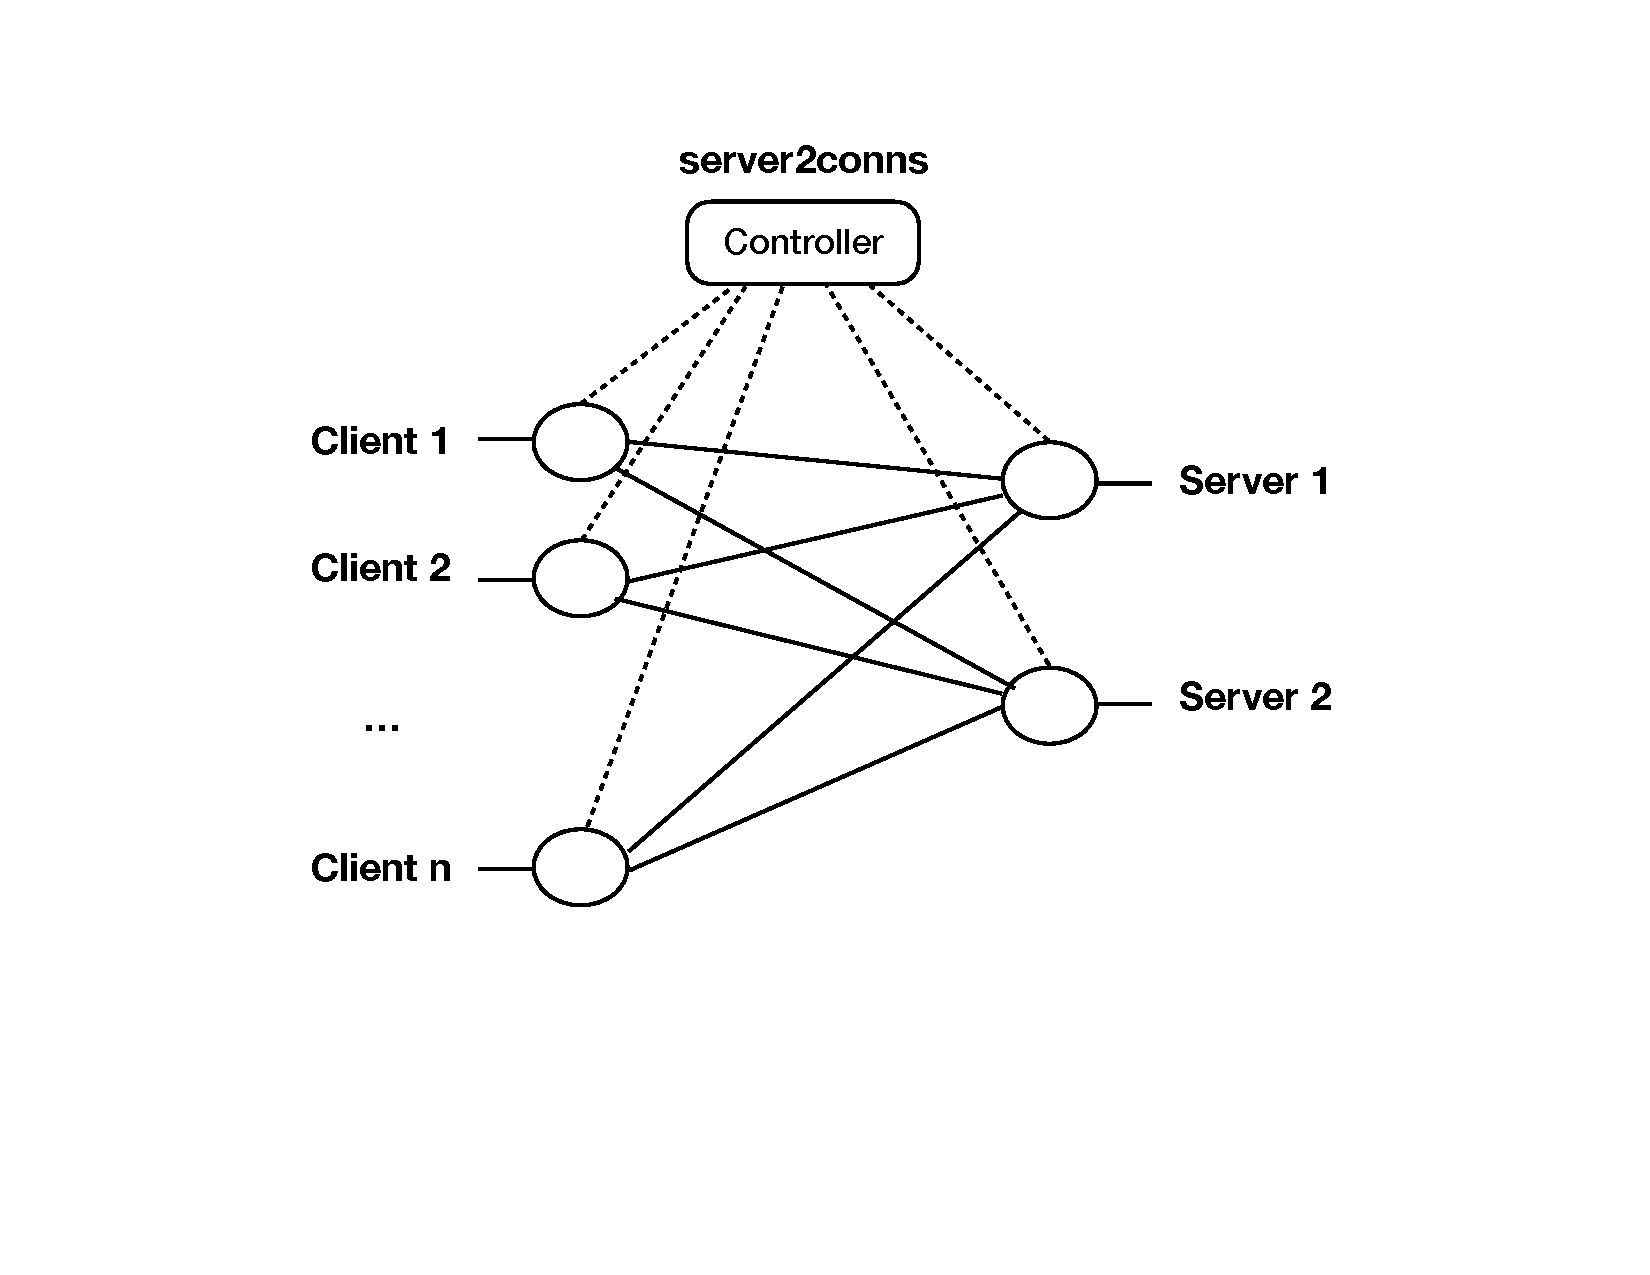
\includegraphics[width=\linewidth]{figures/65.pdf}
%      \caption{\label{fig:lb-example} \small A simple SDN design.}
%\end{subfigure}
%\hspace{0.03\linewidth}
%\begin{subfigure}{0.47\linewidth}
%      \centering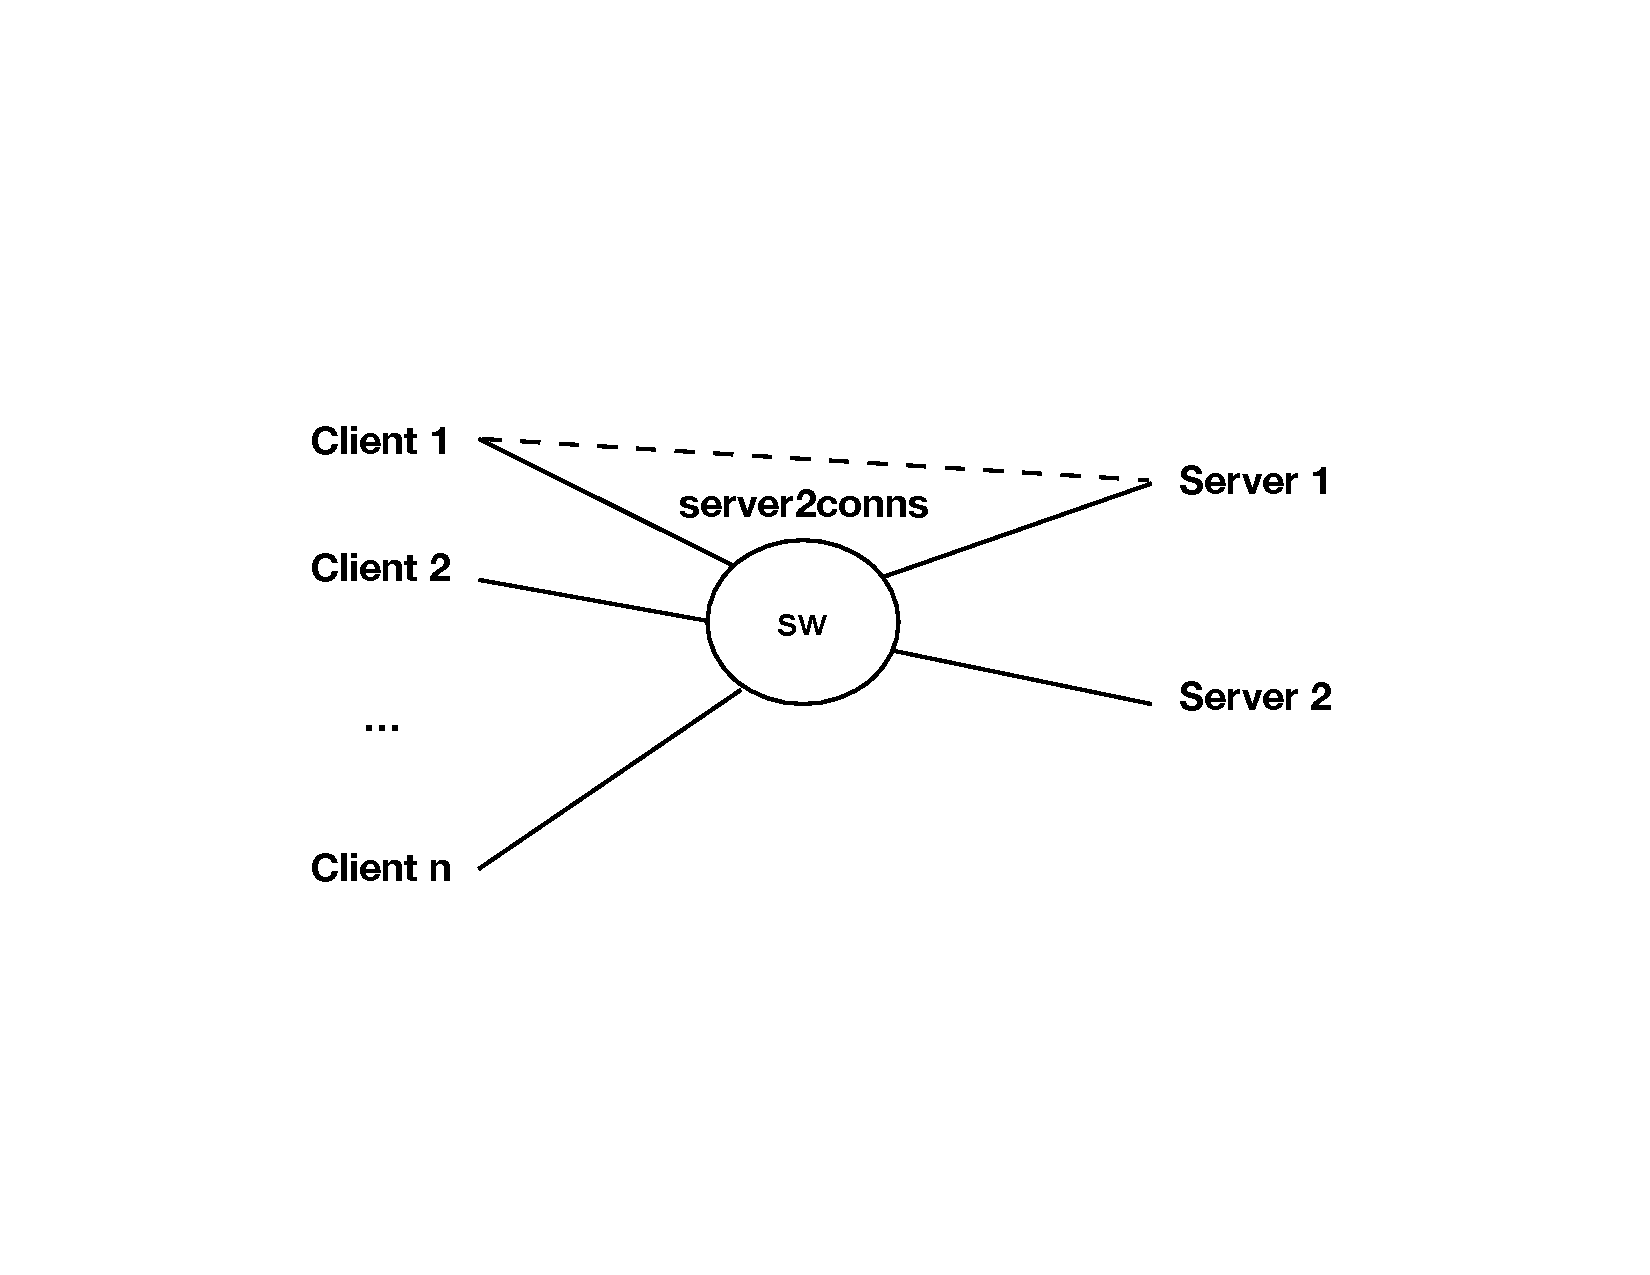
\includegraphics[width=\linewidth]{figures/66.pdf}
%      \caption{\label{fig:fm-example} \small Stateful switch design.}
%\end{subfigure}
%\begin{subfigure}{0.47\linewidth}
%      \centering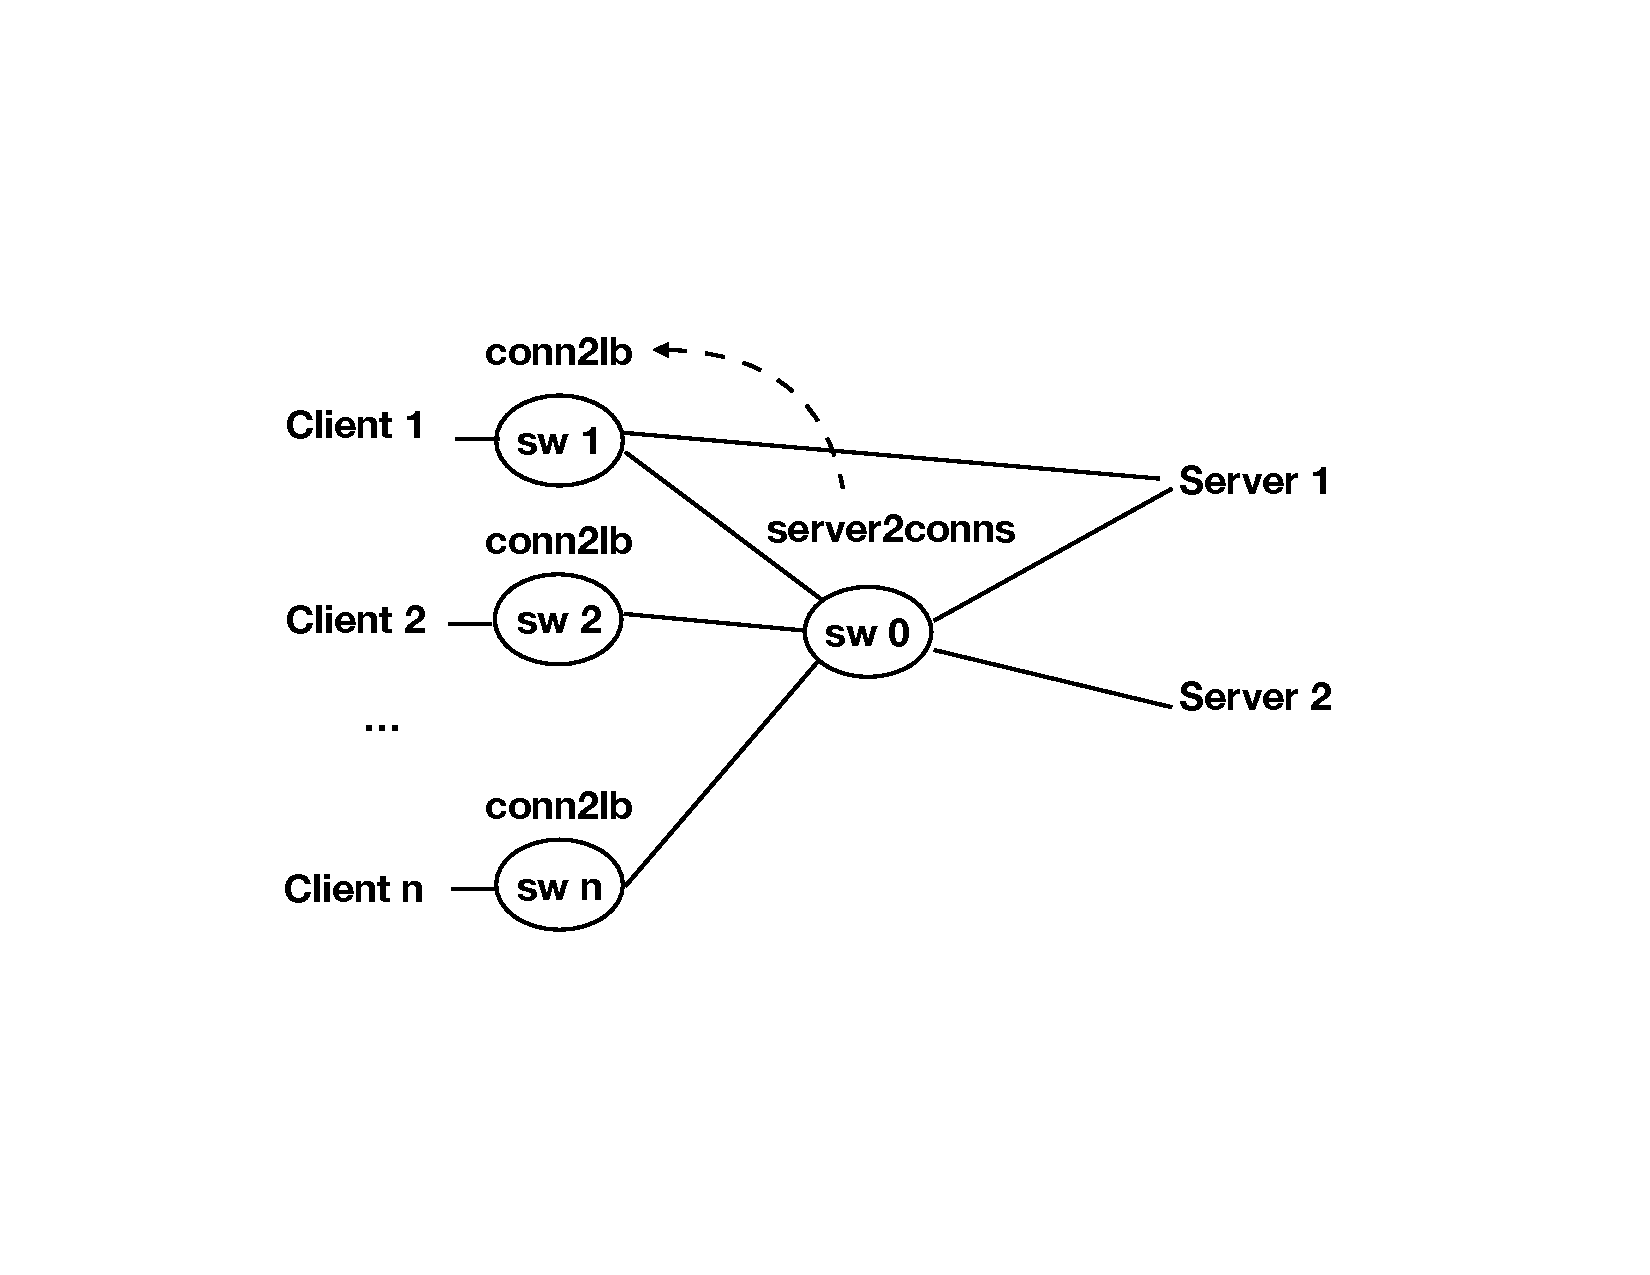
\includegraphics[width=\linewidth]{figures/67.pdf}
%      \caption{\label{fig:fm-example} \small Two-state design.}
%\end{subfigure}
%%\vspace{-2mm}
%%\caption{\footnotesize{The CDF of job latency local and remote jobs.}}
%\caption{\small Examples of load-balancing.}
%%\vspace{-2mm}
%\label{fig:mtv-example}
%\end{figure}
%
%For a simple SDN design, the load-balancing can be done at the controller which keeps a map (denoted as \emph{server2conns}) whose key is a server id and the value is the number of connections currently established for the server. Then, when a client needs to start a new connection, the first packet of the connection will be forwarded to the controller where a server is assigned to the connection based on the map in the controller. The shortage of this design is the latency added for the connection between switches and the controller. By leveraging the stateful switches ([XXX]), the state (\ie, \emph{server2conns}) can be offloaded to the switches where the packets can read states without involving the controller.
%
%A stateful switch design where the load-balancing can be done in the data planes is shown in Figure 1 (b). To achieve the load-balancing in the data planes, the state \emph{server2conns} is kept in the stateful switch $sw$. When a client needs to start a new connection, the first packet will be forwarded to $sw$ where a server will be assigned to the packet (also the state \emph{server2conns} is updated). Then, the packet will be forwarded to the assigned server without involving the controller. The stateful switch design removes the latency between the controller and switches but the paths between clients and servers have a constraint that they must pass through $sw$ even the server has been assigned. (Though the dot line in Figure 1 (b) is the optimal path between $client_1$ and $server_1$, it cannot be used.) This is because \emph{server2conns} is a global variable for all the connections; it cannot be distributed among multiple switches.
%
%To make optimal path available in the stateful switch design, one solution is to change the path after the processing of load-balancing in $sw$(\ie, processing of \emph{server2conns}). To achieve the changing of paths, other state variables are required. As shown in Figure 1 (c), $sw_0$ keeps the state \emph{server2conns} and other stateful switches $sw_1$, $sw_2$, ... $sw_n$ (we assume $client_i$ connects to $sw_i$) keep the states \emph{conn2lb} (each switch maintains \emph{conn2lb}) where the key is the connection and the value is the status of load-balancing (\ie, to indicate whether the load-balancing has been processed for the connection). Consider $client_1$ starts a new connection, the first packet will arrive at $sw_1$. Based on \emph{conn2lb}, if the status of the connection indicates the server is not assigned, then the packet will be forwarded to $sw_0$. After the processing in $sw_0$, it updates the state \emph{conn2lb} in $sw_1$ to set the value to indicate the load-balancing is done. Then, based on \emph{conn2lb} in $sw_1$, all the following packets from $client_1$ to the server can use the optimal path which may not pass through $sw_0$.
%
%Though the two-state design resolves the issues of other designs (\ie, additional latency and not optimal path), this cannot be implemented with existing work. The most relevant work, SNAP [XXX], achieves a network-wide stateful packet processing, but the data dependency between \emph{conn2lb} and \emph{server2conns} (\ie, packet reads \emph{conn2lb}; packet reads \emph{server2conns}; packet writes \emph{conn2lb}) makes the two state variables must be assigned in a single stateful switch, which cannot achieve the optimal path requirement. Therefore, in this paper, we propose the general network-wide stateful packet processing which provides a high flexibility for the state updates of stateful packet processing.







\section{\concept{} Overview} \label{sec:system}
In this section, we first give the programming model of \concept{}, followed by
its architecture, and the workflow to transform a high-level SDC program to
datapath configurations with local state sharing.

%including the translation from programs into flow rules at switches and configurations of middleboxes (\ie, how to interact with switches). We will start with the extension of programming model from SNAP (XXX) and then describe each component of the system.

\vspace{-2mm}
\subsection{Programming Model}
\concept{} adopts an omnipotent programming model proposed in high-level SDN
programming systems (\eg, Maple~\cite{maple}), which logically programs every single packet with an
onPacket function. In addition to the primitives that read and test on packet
headers, \concept{} designs the following primitives for users to model and
specify middleboxes in SDC network. The first is to specify a middlebox in the network (\codeword{m = middlebox(name,
property)}) where the property indicates the middlebox is stateless or not; The
second is to
invoke the packet handling of a middlebox (\codeword{m.handle(pkt)}).
Specifically, we consider a middlebox as a packet handling function that can
return the result for the incoming packet. For the stateless middlebox, if two
packets have the same 5-tuple match fields, they always have the same
results. For the stateful middlebox, this cannot be guaranteed as the packet
processing depends on the state in the middlebox.

%To handle the returned result of a middlebox for a packet, we consider the
%following switch-middlebox interaction process. 
In \concept{}, the interaction between switch and middlebox is bi-directional.
A switch can send a packet to a
middlebox for the processing through a tunnel. After the processing, the middlebox can send
the packet back and share its local state of the packet %(5-tuple flow matches)
with switches. In \concept{}, such interaction is transparent to the user so that
the user does not need to manually configure the local state sharing between
data plane devices. Instead, as we will show in the next section, \concept{}
automatically translates high-level SDC programs into data plane configurations
with local state sharing.

%To reUser is unaware of such interaction. Instead,

%is transparent to the user. 
%(leveraging their stateful datapath design). %Note that by using
%tunnels, any switch can send a packet to any middlebox, and also the inverse.

%Though the interaction is simple, there are several details need to consider
%(\eg, in the step 3 of the \concept{} design for the firewall example, how to
%guarantee that the packet gets the newest state?). We will talk about the
%details in the next section.

In addition to the middlebox primitives, \concept{} also adopts the route algebra
primitive~\cite{gao2018t} for the user to specify path constraints for packets
forwarding in SDC network. The abstract syntax of the \concept{} programming model
is shown in Fig~\ref{fig:grammar1}. Specifically, for the route algebra expressions, we adopt the same in~\cite{gao2018t}. For the middlebox, programmers can specify its property, \ie, stateless or stateful. 
%Inside the onPacket program, besides the basic packet test statements, programmers can specify a middlebox operation to handle packets. Also the route algebra variable should be the return as it gives the path constraints.

%Therefore, we consider the three kinds of statements
%(besides the basic control statements such as \codeword{if, else}): 1. Test of
%packet match fields; 2. Packet handling of a middlebox; 3. Route algebra as a
%return.

\begin{figure}[ht]
{%\small
% \fontsize{10}{12}\selectfont 
\scriptsize
%{\bf Abstract syntax:}
%\vspace{-2mm}
\[%\arraycolsep=1.4pt\def\arraystretch{2.2}
\begin{array}{rclr}
p &\bnfdef & \ONPKT\ \{I\},\ d_1,\ \ldots,\ d_n &(\textit{program})\\
d &\bnfdef & x^r\ =\ r\  & (\textit{route algebra decl})\\
 & & \bnfalt x^m\ =\ middlebox(n,\ s) & (\textit{middlebox decl})\\
I &\bnfdef & x\ =\ e & \\
 & & \bnfalt I;I &  (\textit{sequencing})\\
 & & \bnfalt x\ =\ x^m.handle(pkt) &  (\textit{middlebox operation})\\
 & & \bnfalt \ifelse{e^b}{I}{I} &  (\textit{conditional})\\ %\\ 
 & & \bnfalt \return{x^r} \bnfalt \return{r} &  (\textit{func return})\\ 
% & & \bnfalt m[e_1, \dots, e_n] := e & (\textit{map update}) \\
% & & \bnfalt s := s \cup \{e\} \bnfalt s := s - \{e\} & (\textit{set update}) \\
e &\bnfdef & c \bnfalt x &  (\textit{consts, vars})\\
%& & \bnfalt x^r  & (\textit{route algebra vars}) \\
& & \bnfalt x^m & (\textit{middlebox vars}) \\
& & \bnfalt pkt.a & (\textit{packet fields}) \\
% & & \bnfalt e+e \bnfalt e*e \dots & (\textit{arith}) \\ 
e^r & \bnfdef & e == e \bnfalt e \leq e \dots & (\textit{relational})\\
e^b & \bnfdef & e^r \bnfalt e^r\ \&\ e^r \bnfalt e^r\ |\ e^r \dots & (\textit{boolean})\\
(r &{\color{blue}{\in}}&\mathit{route\ algebra\ expressions}) & \\
(c &{\color{blue}{\in}}& \mathit{strings}) & (\mathit{consts})\\
(a &{\color{blue}{\in}}& \{ \mathit{macSrc}, \mathit{ipDst} \dots \}) & (\textit{packet fields})\\
(n &{\color{blue}{\in}}& \mathit{strings})  &  (\textit{middlebox names})\\
(s &{\color{blue}{\in}}& \{ \mathit{stateless},\mathit{stateful} \})  &  (\textit{properties})\\
(x &{\color{blue}{\in}} & \{\tx_1,\tx_2,\dots,\ty_1,\dots\}) &  (\textit{variables})\\
\end{array}\]}% small
%\vspace{1mm}
% \hrule
%\vspace{-5mm}
\caption{\concept{} abstract syntax.}
\label{fig:grammar1}
\end{figure}



\para{Example \concept{} program:} Revisit the motivating example in Section~\ref{sec:motivation}, the network
operator can specify the policy to forward packets of sensitive and non-sensitive data along different paths using the \concept{} program in Fig.~\ref{fig:code}.
%to forward packets of sensitive and non-sensitive data along different paths using the \concept{} program in Fig.~\ref{fig:code}.

\begin{figure}[h]
\begin{scriptsize}
\begin{verbatim}
L1: mFW = middlebox("firewall", "stateless")
L2: PATH1 = h1 -> b -> h2 //b: waypoint
L3: PATH2 = h1 -> c -> h2 //c: waypoint
L4: //any: picking any path
L5: def onPacket(pkt):
L6:   if pkt.srcAddr == h1 & pkt.dsrAddr == h2:
L7:     if mFW.handle(pkt) == SENSITIVE:
L8:       return any(SPC.stable + PATH1)
L9:     else:
L10:      return any(SPC.stable + PATH2)
L11:  else: return DROP
\end{verbatim}
\end{scriptsize}
	\caption{\small The \concept{} program for the policy in the motivating example. For line 8 (9), the correct versions are in their comments.}
\label{fig:code}
\end{figure}

Specifically, line 2 (3) specifies a path constraint that starts from $h_1$ to $h_2$ and must pass through $b$ ($c$) (Note that it does not represent a concrete path but a path constraint). And the return statements use \emph{any} function (defined in route algebra~\cite{gao2018t}) that picks any path satisfying the constraint. Although the programming model is quite simple, as involving middleboxes which physically map to nodes in the network, the system needs to guarantee the correctness for the program.

\para{Correctness}: We denote the correctness as the following: For any packet $pkt$, the real forwarding path for $pkt$ in the network must comply with the returned path for $pkt$ in the program. For example, if the programmer uses \emph{opt} function to pick the shortest hop count path with the constraint (\ie, \codeword{opt(PATH1)}), then the returned path is $gw, a, b, d$. However, as the (first) packet must access the firewall, the real path must include $fw$ which does not comply with the returned path in the program.

One simple solution to guarantee the correctness is to let the programmer explicitly include the necessary middlebox nodes in the path constraint. In this case, it should be \codeword{PATH1 = h1 -> fw -> b -> h2}. However, this can add extra burden to programmers that they should make sure the path constraints comply with the traces of packets in the network.

\para{System Path Constraint}: To resolve the issue, we introduce the System Path Constraint (SPC) which is a global variable storing path constraints that must be complied with when computing a path at any location in the program. The intuition is that when a packet going through the program, some statements can add path constraints for the packet. For example, in Fig.~\ref{fig:code}, line 6 adds a constraint that the path should start from $h_1$ to $h_2$; Line 7 adds a constraint that the path must include the firewall. Then, after line 7, the SPC variable includes constraints that the path starts from $h_1$ to $h_2$ and includes $fw$. If the line 8 uses the \emph{opt} function, then it should be \codeword{return opt(SPC + PATH1)} where the ``+'' means connecting the waypoints constraints in SPC and PATH1, and its result is $gw, fw, a, b, d$. (Note that the definition of \codeword{SPC.stable} will be given in the next section.)

%And the programmer should include the SPC variable when computing the path in line 8 (\ie, \codeword{return any(SPC + PATH1)} where the ``+'' means connecting the waypoints constraints in SPC and PATH1). As such, the result of \codeword{opt(SPC + PATH1)} should be $gw, fw, a, b, d$.

%
%\begin{figure}[h]
%\begin{footnotesize}
%\begin{verbatim}
%L1: mFW = middlebox("firewall")
%L2: PATH1 = h1 -> mFW -> b -> h2 //b: waypoint
%L3: PATH2 = h1 -> mFW -> c -> h2 //c: waypoint
%L4: opt := picking shortest hop count path
%L5: def onPacket(pkt):
%L6:     if pkt.srcAddr == h1 & pkt.dsrAddr == h2:
%L7:         if mFW.handle(pkt) == SENSITIVE:
%L8:             return opt(PATH1) 
%L9:         else:
%L10:           return opt(PATH2)
%L11:    else: return DROP
%\end{verbatim}
%\end{footnotesize}
%	\caption{\small The \concept{} program for the policy in the motivating example.}
%\label{fig:code}
%\end{figure}
%
%\begin{figure}[h]
%\begin{footnotesize}
%\begin{verbatim}
%L1: mFW = middlebox("firewall")
%L2: PATH1 = h1 -> b -> h2 //b: waypoint
%L3: PATH2 = h1 -> c -> h2 //c: waypoint
%L4: opt := picking shortest hop count path
%L5: def onPacket(pkt):
%L6:     if pkt.srcAddr == h1 & pkt.dsrAddr == h2:
%L7:         if mFW.handle(pkt) == SENSITIVE:
%L8:             return opt(SPC.stable + PATH1) 
%L9:         else:
%L10:           return opt(SPC.stable + PATH2)
%L11:    else: return DROP
%\end{verbatim}
%\end{footnotesize}
%	\caption{\small The \concept{} program for the policy in the motivating example.}
%\label{fig:code}
%\end{figure}

%Since we do not focus on the state operation deployment (which is the major component of SNAP), we only considers two kinds of statements that can apply to packets: 1. Test of packet match fields (\eg, line 6 in the firewall program); 2. Packet handling of middlebox (\eg, line 7 in the firewall program). The former one is the same with the SNAP and the latter one returns the result of packet handling of a middlebox.

%
%Also, as only stateless middleboxes can leverage stateful switches as the cache of results of its packet processing, the system needs to identify whether a middlebox is stateless or not. For simplicity, we make the programmer give the hint. In the program, when initializing a middlebox variable, the program should specify whether it is stateless or not. The following gives an example that how to give a hint at the middlebox variable initializing statement.
%
%\begin{small}
%\begin{verbatim}
%mFW = middlebox("firewall", "stateless")
%...
%if mFW.handle(pkt) = GOOD:
%\end{verbatim}
%\end{small}
%
%
%\subsection{Middlebox Behavior}
%
%We consider a middlebox as a packet handling function that can return the result for the incoming packet. For the stateless middlebox, if two packets have the same 5-tuple match fields, then they always have the same results. For the stateful middlebox, this cannot be guaranteed as its packet processing depends on the state in the middlebox.
%
%For the interaction between a middlebox and a switch, we consider the following model. A switch can send a packet to a middlebox for the processing, and after the processing the middlebox can send the packet back and update a flow's state (based on the result) at any switch. (The flow has the same 5-tuple with the packet.) This process is very similar with the interaction between OpenFlow switches and the controller which includes packet-in message, packet-out message, and OpenFlow rules update. Note that by using tunnels, any switch can send a packet to any middlebox, and also the inverse. Though the interaction is simple, there are several details need to consider (\eg, in the step 3 of the \concept{} design for the firewall example, how to guarantee that the packet gets the newest state?). We will talk about the details in the next section.

\vspace{-2mm}
\subsection{Architecture and Workflow}
Fig.~\ref{fig:system-workflow} presents the architecture and workflow on how
\concept{} translates high-level \concept{} SDC programs to low-level
configurations of data plane devices with local state sharing. Given a
high-level \concept{} SDC program, \concept{} first computes a decision graph that captures the forwarding decisions process of
packets and stateful operations on packets. Second, \concept{} computes optimal
paths for packet forwarding in the network with a system defined objective (\eg,
maximizing total throughput). \textbf{Note} that the system computes paths when the returned paths are not concrete (\eg, using $any$ function), and in the remaining part of the paper, we assume these paths are not concrete to introduce the path computation part. Third, the device-level data plane configurations are generated, which
include local state sharing configurations, so that devices can exchange local
state to forward the packets along the computed optimal paths. \concept{} leverages the stateful switch for local state sharing which includes two match-action tables: one is
a state table (\ie, $match \rightarrow state$) and the other is a match table
(\ie, $match+state \rightarrow action$). Given a switch, a
packet first enters the state table to get its corresponding state (by matching
its packet fields) and then enters the match table to get the action.

%from the program (and the definition of DG
%will be shown in the next section). Step 2: Based on the DG and the topology,
%Step 3: Generate datapath configuration in the network.

\begin{figure}[!htbp]
%\vspace{-2mm}
\centering
\begin{subfigure}{0.4\linewidth}
      \centering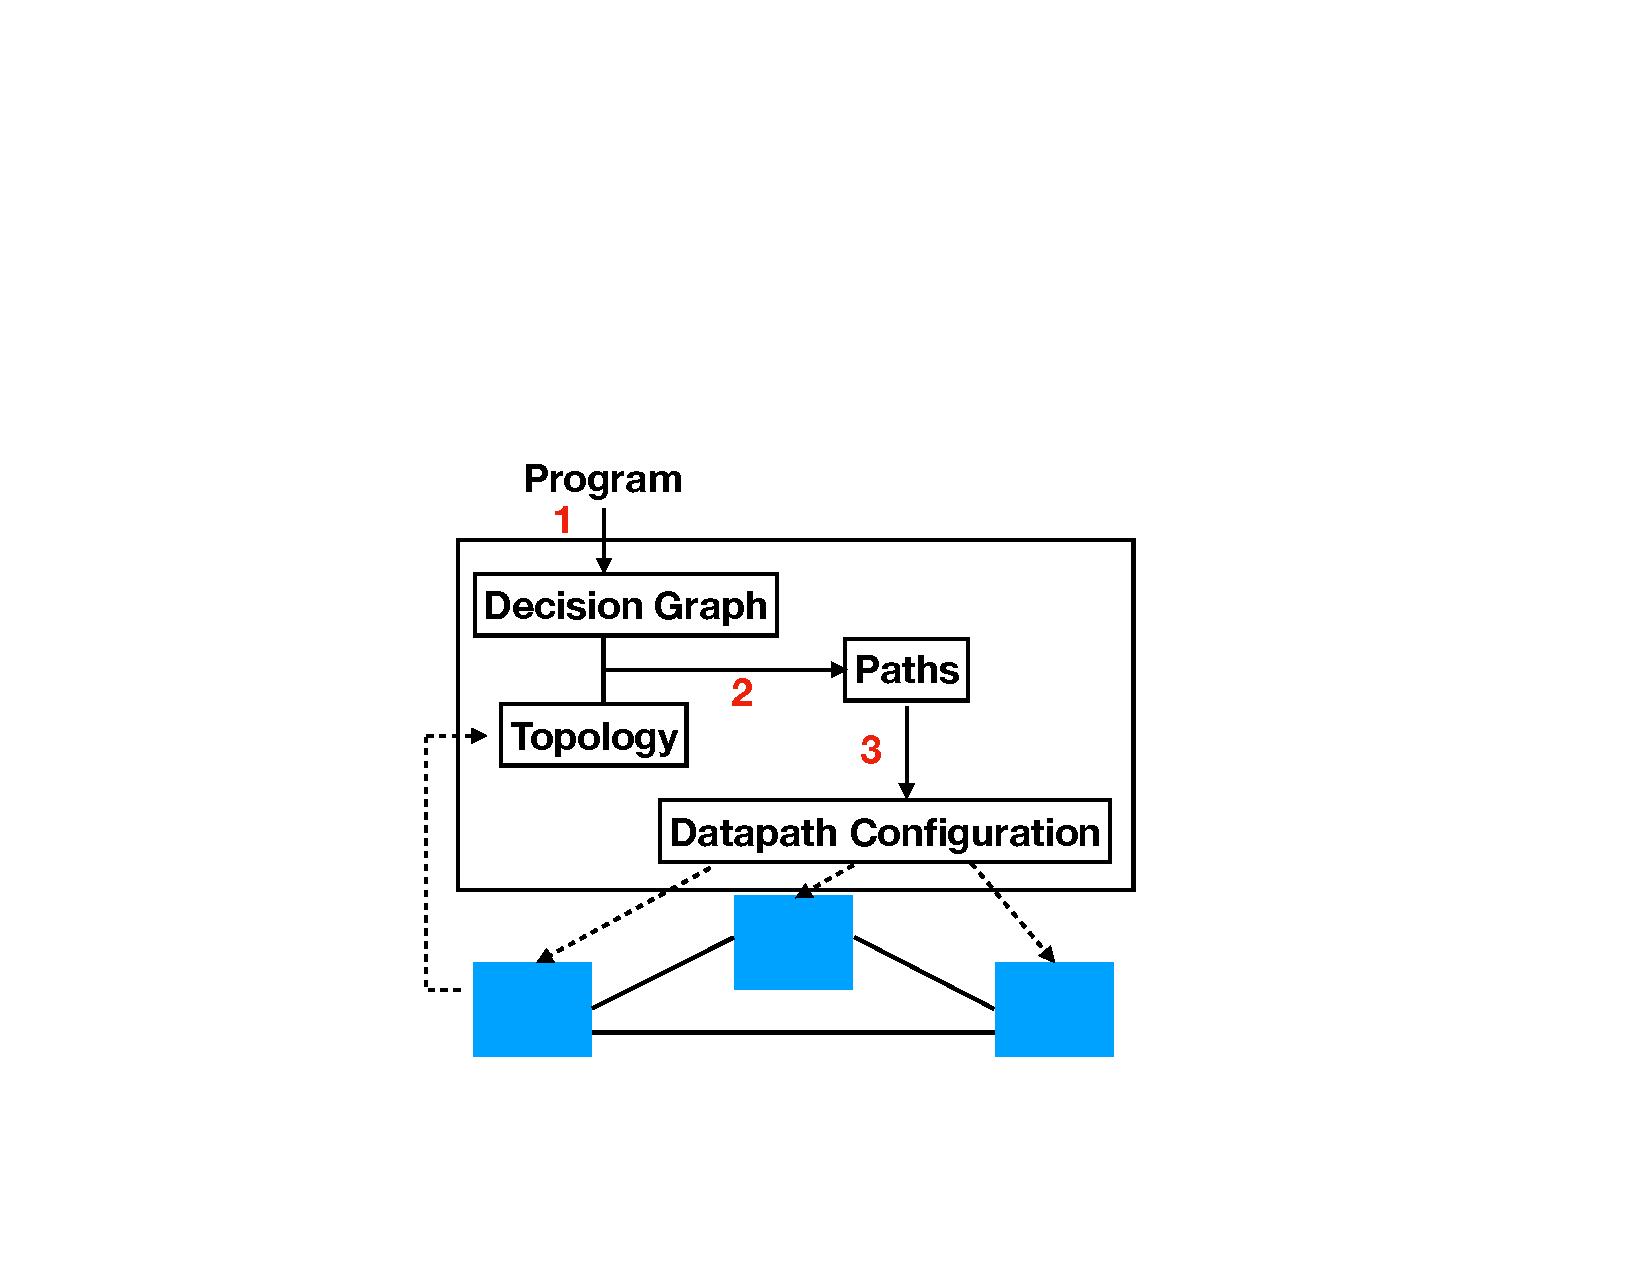
\includegraphics[width=\linewidth]{figures/ss-125.pdf}
\end{subfigure}
%\vspace{-2mm}
%\caption{\footnotesize{The CDF of job latency local and remote jobs.}}
\caption{\small The architecture and workflow of \concept{}.}
%\vspace{-2mm}
\label{fig:system-workflow}
\end{figure}

\begin{figure}[!htbp]
%\vspace{-2mm}
\centering
      \centering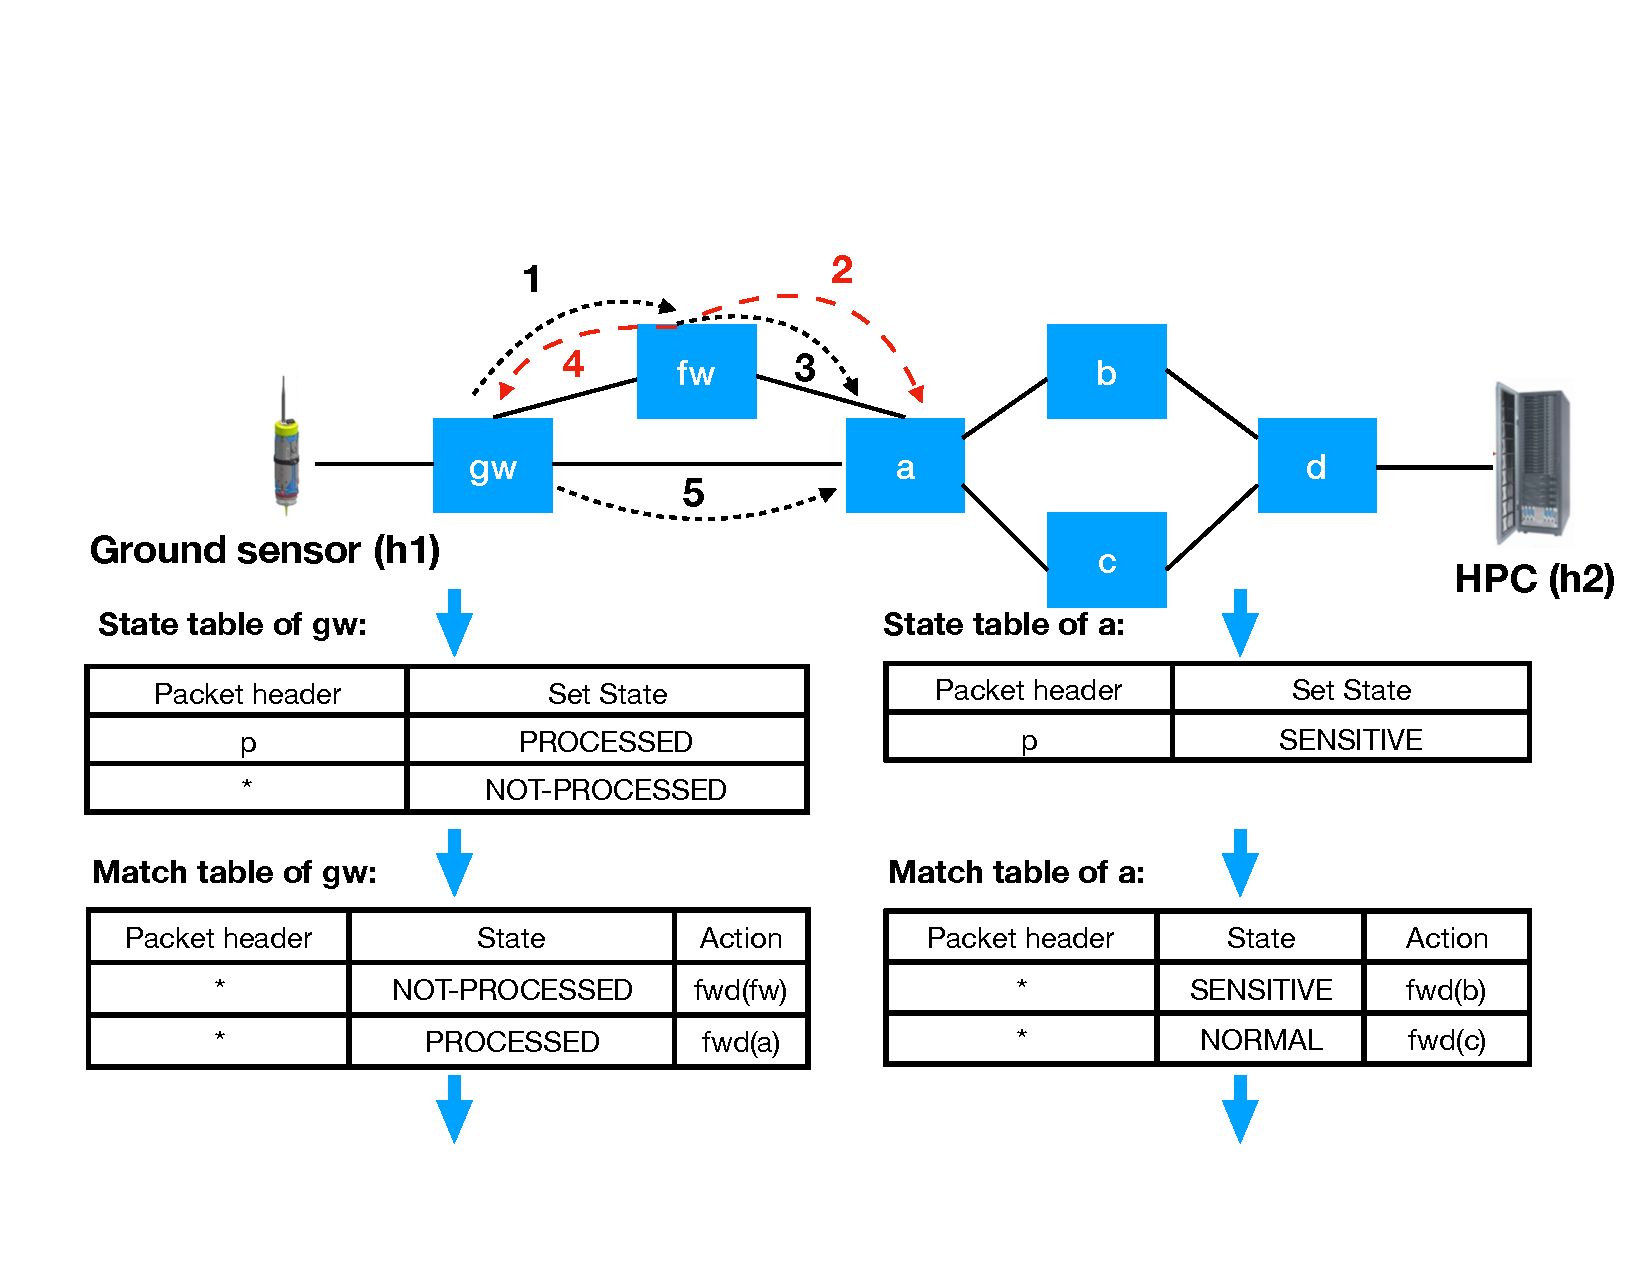
\includegraphics[width=0.8\linewidth]{figures/ss-124.pdf}
   %\vspace{-2mm}
%\caption{\footnotesize{The CDF of job latency local and remote jobs.}}
	\caption{\small The configuration translated by \concept{} from the
	program in Fig.~\ref{fig:code}.}
%\vspace{-2mm}
\label{fig:dsdc-result}
\end{figure}

\para{Example configuration with local state sharing}:  
Fig.~\ref{fig:dsdc-result} gives the data plane configuration with local state
sharing translated from the SDC program in Fig.~\ref{fig:code}. Specifically,
by allowing the local state sharing, the
firewall $fw$ can share its local identification state for a flow with the
gateway switch $gw$.
For example, it can send the state: 
$srcAddr=h1,dstAddr=h2,srcPort=12345,dstPort=22,protocol=tcp \rightarrow$
\emph{PROCESSED} to $gw$, which can insert it into its state table.

With this configuration, the first packet $p$ arrives at the
gateway $gw$ is forwarded to $fw$ by getting a state
\emph{NOT-PROCESSED} at $gw$ (Step 1). Assume $fw$ identifies $p$ as \emph{SENSITIVE}.
It first sends this local state $p \rightarrow SENSITIVE$ to $a$ (Step 2). Next,  $fw$
forwards $p$ to $a$ (Step 3), where $p$ is forwarded to $b$ because its state is \emph{SENSITIVE}. 
Then $fw$ sends the local state $p \rightarrow PROCESSED$ to $gw$ (Step 4). As such, all future packets with the
same match fields as $p$ entering $gw$ will be forwarded directly to $a$ (Step 5).

%design which leverages this local state
%sharing. We assume 



%The design with \concept{} has 5 steps: 

 



%
%In this section, we will first give basic concepts and the target for general network-wide stateful packet processing in data planes. Then, the consistency requirement will be discussed based on the basic concepts.
%
%\subsection{basic concepts and the target}
%
%\para{State variable and operations}: State variables are the persistent states on the data planes (stateful switches). In this paper, for the simplicity, we consider the state variable as a key-value map whose key can be matched by the fields of packets. For the read operation of state variables, an incoming packet ($pkt$) can read a value of an entry in the map ($m$) and store the value to the packet's meta data [ref: meta data XXX] by matching the fields ($f$) of the packet (note that the fields include meta data); for the write operation, flow tables can support a special state-update action that can update the map (including modify the value of a specific entry in the map and/or add a new entry to the map). 
%
%%The formal expressions of the two operations are shown in the Figure 2 XXX.
%
%%Figure formal expression.
%
%\para{General network-wide stateful packet processing}: Network-wide stateful packet processing for a packet can be viewed as a sequence of read/write operations of the state variables applied by the packet. Given a state variable (map) $m_k$, we denote $o_i^{s(i)}$ as the operation with $m_k$ indicated by $s(i) = k$. Then, we have a sequence of $n$ operations (denoted as $O$) as $o_1^{s(1)}, o_2^{s(2)}, ..., o_i^{s(i)}, ..., o_n^{s(n)}$. 
%We denote a sequence of operations $O$ with at most two operations $o_i^{s(i)}, o_j^{s(j)}$ in $O$ that they have $s(i) = s(j) = k$ and $i \neq j$ as \emph{one-loop} sequence for $m_k$ and $o_i^{s(i)}, o_j^{s(j)}$ as its \emph{end-loop} operations.
%For the existing work (\ie, SNAP), for any \emph{one-loop} sequence, all the state variables (\ie, maps) involved in the sequence between its \emph{end-loop} operations (including \emph{end-loop} operations) should be stored in a \textbf{single} switch. 
%This is why it cannot achieve the load-balancing example in Sec. 1. 
%
%\para{Target}: For the proposed \textbf{general} network-wide stateful packet processing, we relax the constraint of single switch and our target is to support a more flexible sequence of read/write operations with less constraints for putting which state variables to which switches. (Note that a state variable should be placed on a single stateful switch.) Specifically, given a state variable $m_k$ and a flow with requirements to access $m_k$, the flow can apply at most one \emph{one-loop} sequence for $m_k$ where the state variables involved in the operations between its \emph{end-loop} operations can be spread to \textbf{multiple} switches. For the example in Figure 2, state variable $m_k$ is $sw_1$ and two flows $flow_1$ and $flow_2$ access $m_k$. Flow $flow_1$ has two sequences of operations: $op_{11}, op_{12}, op_{13}$ and $op_{11}, op_{12}, op_{14}, op_{15}$. Both sequences are \emph{one-loop} sequences for $m_k$ as all $op_{11}, op_{13}, op_{15}$ involve $m_k$. Then, this is not supported in our target. If $flow_1$ only keeps $op_{11}, op_{12}, op_{13}$, then the sequence of operations of $flow_2$ also can be supported.
%
%However, this flexibility may arise consistency issue which will be discussed in the following subsection.
%
%\begin{figure}[!htbp]
%%\vspace{-2mm}
%\centering
%\begin{subfigure}{0.7\linewidth}
%      \centering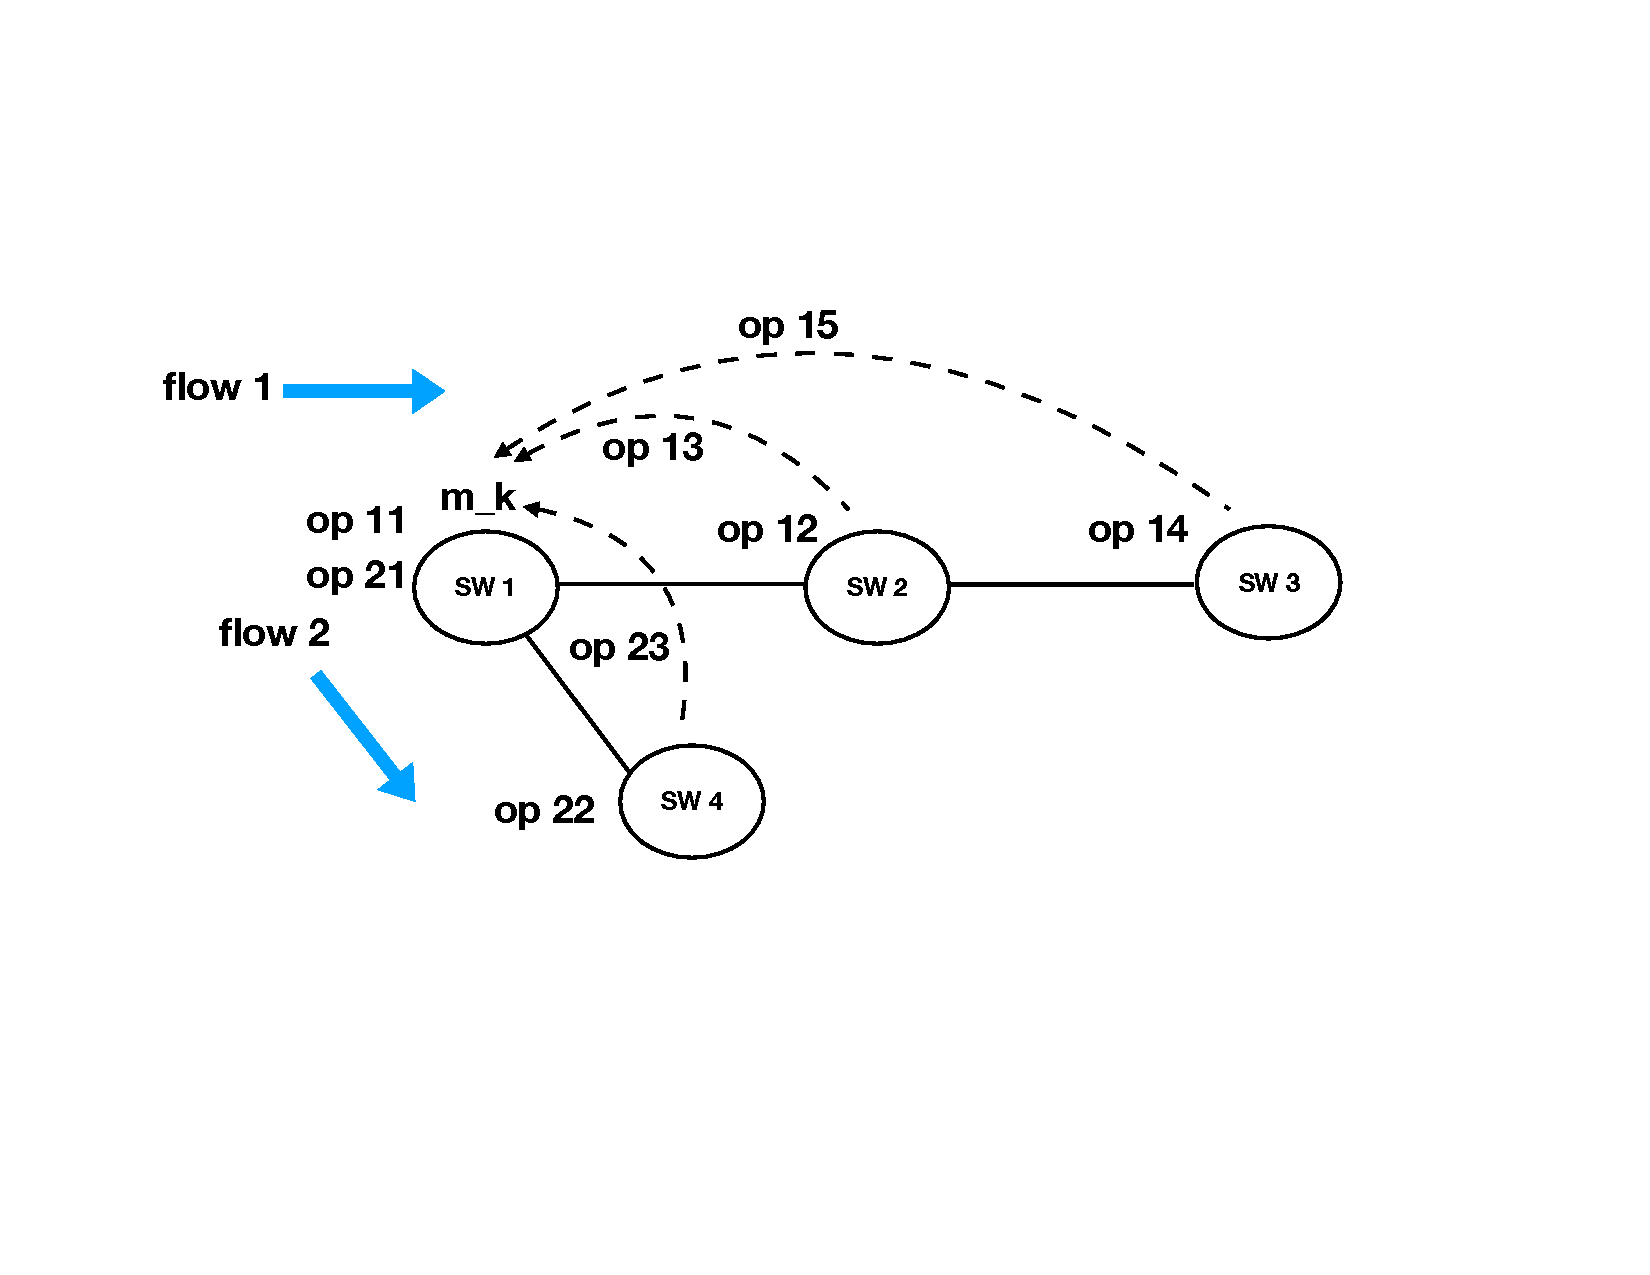
\includegraphics[width=\linewidth]{figures/68.pdf}
%\end{subfigure}
%%\vspace{-2mm}
%%\caption{\footnotesize{The CDF of job latency local and remote jobs.}}
%\caption{\small Example of \emph{one-loop} sequence.}
%%\vspace{-2mm}
%\label{fig:mtv-example}
%\end{figure}
%
%\subsection{consistency requirement}
%
%%As a flow consists of a sequence of packets, for any event caused by a packet, the event should be noticed by the following packets in the flow. In the stateful packet processing setting, we should have the following consistency requirement. 
%
%First, consistency should be considered when a packet $pkt_i$ (belonging to a flow with a sequence of packets $pkt_1, pkt_2, ..., pkt_i, ...$ where a packet with a smaller index appears at the network earlier) tries to access a state variable $m_k$. We denote the sequence of historical state operations of $pkt_i$ as $HO(pkt_i)$. Also, we have a sequence of packets $pkt_{i1}, pkt_{i2}, ..., pkt_{ih}$ (denoted as $D(pkt_i)$) as a subsequence of $pkt_1, pkt_2, ..., pkt_{i-1}$ that $\forall pkt_{ij} in D(pkt_i), HO(pkt_i) is the prefix of HO(pkt_{ij})$. Then, the consistency requirement is that $\forall pkt_{ij} \in D(pkt_i)$, for the value of $m_k$ updated by $pkt_{ij}$, $pkt_i$ must see the updated value of $m_k$. In other words, if $pkt_{i-1}$ and $pkt_i$ following the same path with the same state operations to a stateful switch $sw$, $pkt_i$ (and the following packets) must see any update to any state variables at $sw$ as long as these updates comes from $pkt_{i-1}$. If two packets do not have the same historical state operations, as the order of the two packets itself cannot guarantee, the consistency also should not be considered.
%
%%Given a flow with a sequence of packets $pkt_1, pkt_2, ..., pkt_i, ...$ (a packet with a smaller index appears at the network earlier) and a set of state variables (maps) $M$, we denote the value of $M$ as $M_i$ if it is just before $pkt_i$ is processed by a sequence of state operations with $M$ and $M_i'$ if it is just after $pkt_i$ is processed. Then, the consistency requirement is: $\forall pkt_i, M_i = M_{i-1}'$ ($M_0$ means the original states). In other words, if $pkt_i$ updates any states, $pkt_{i+1}$ (and the following packets) should see the updated states.
%
%In a simple SDN network, the consistency requirement is easy to guarantee as all the states are in the logical centralized controller. Also, the consistency in the single switch design for \emph{one-loop} sequences is also easy to achieve as a single switch can store complex data dependency among state variables.
%%given a sequence of state operations $O$, if there are any two operations with the same state variable in $O$ and all the state variables between these two operations are placed in a single switch
%%the consistency is also easy to guarantee if all the state variables between these two operations are placed in a single switch. 
%However, in the proposed general network-wide stateful packet processing, it is not easy to guarantee as a packet can jump to the previous switch to update a state variable that has been updated before by the packet. We will discuss how the consistency guaranteed in the following section.
%





\section{Design Details}\label{sec:details}

In this section, we present the details of \concept{}. We
first give the details of decision graph, followed by the path
computation and the data path generation. 

\vspace{-2mm}
\subsection{Decision Graph}

The Decision Graph (DG) is used to capture the forwarding decisions process of
packets and stateful operations on packets. 
%capture the trace of every packet applied by the program. The trace is the decision dependencies (\ie, the results of packet fields test statements and middlebox processing statements) of a packet and its returned path (\ie, path constraints). In this paper, we focus on the waypoints constraint (\ie, a sequence of nodes in the network that packets should pass through) as it would complicate the path computation involving the stateful middleboxes. 
We define a DG as a directed acyclic graph (with a single root) that has three types of nodes: packet-test nodes, middlebox-operation nodes, and action nodes (mapping to three basic primitives, packet-test, middlebox, and route algebra). The first two nodes are the internal nodes of DG while the last one is the leaf node. An out-edge of a node can specify a range of packets (if the node is a packet-test node) or a result from a middlebox (if the node is a middlebox-operation node). For example, the DG of the motivating program is shown in Fig.~\ref{fig:dg-example}. Note that we do not focus on the computation of DG from a program which can be achieved by existing (compiler) work~\cite{arashloo2016snap}~\cite{smolka2015fast}.

\begin{figure}[!htbp]
%\vspace{-2mm}
\centering
\begin{subfigure}{0.8\linewidth}
      \centering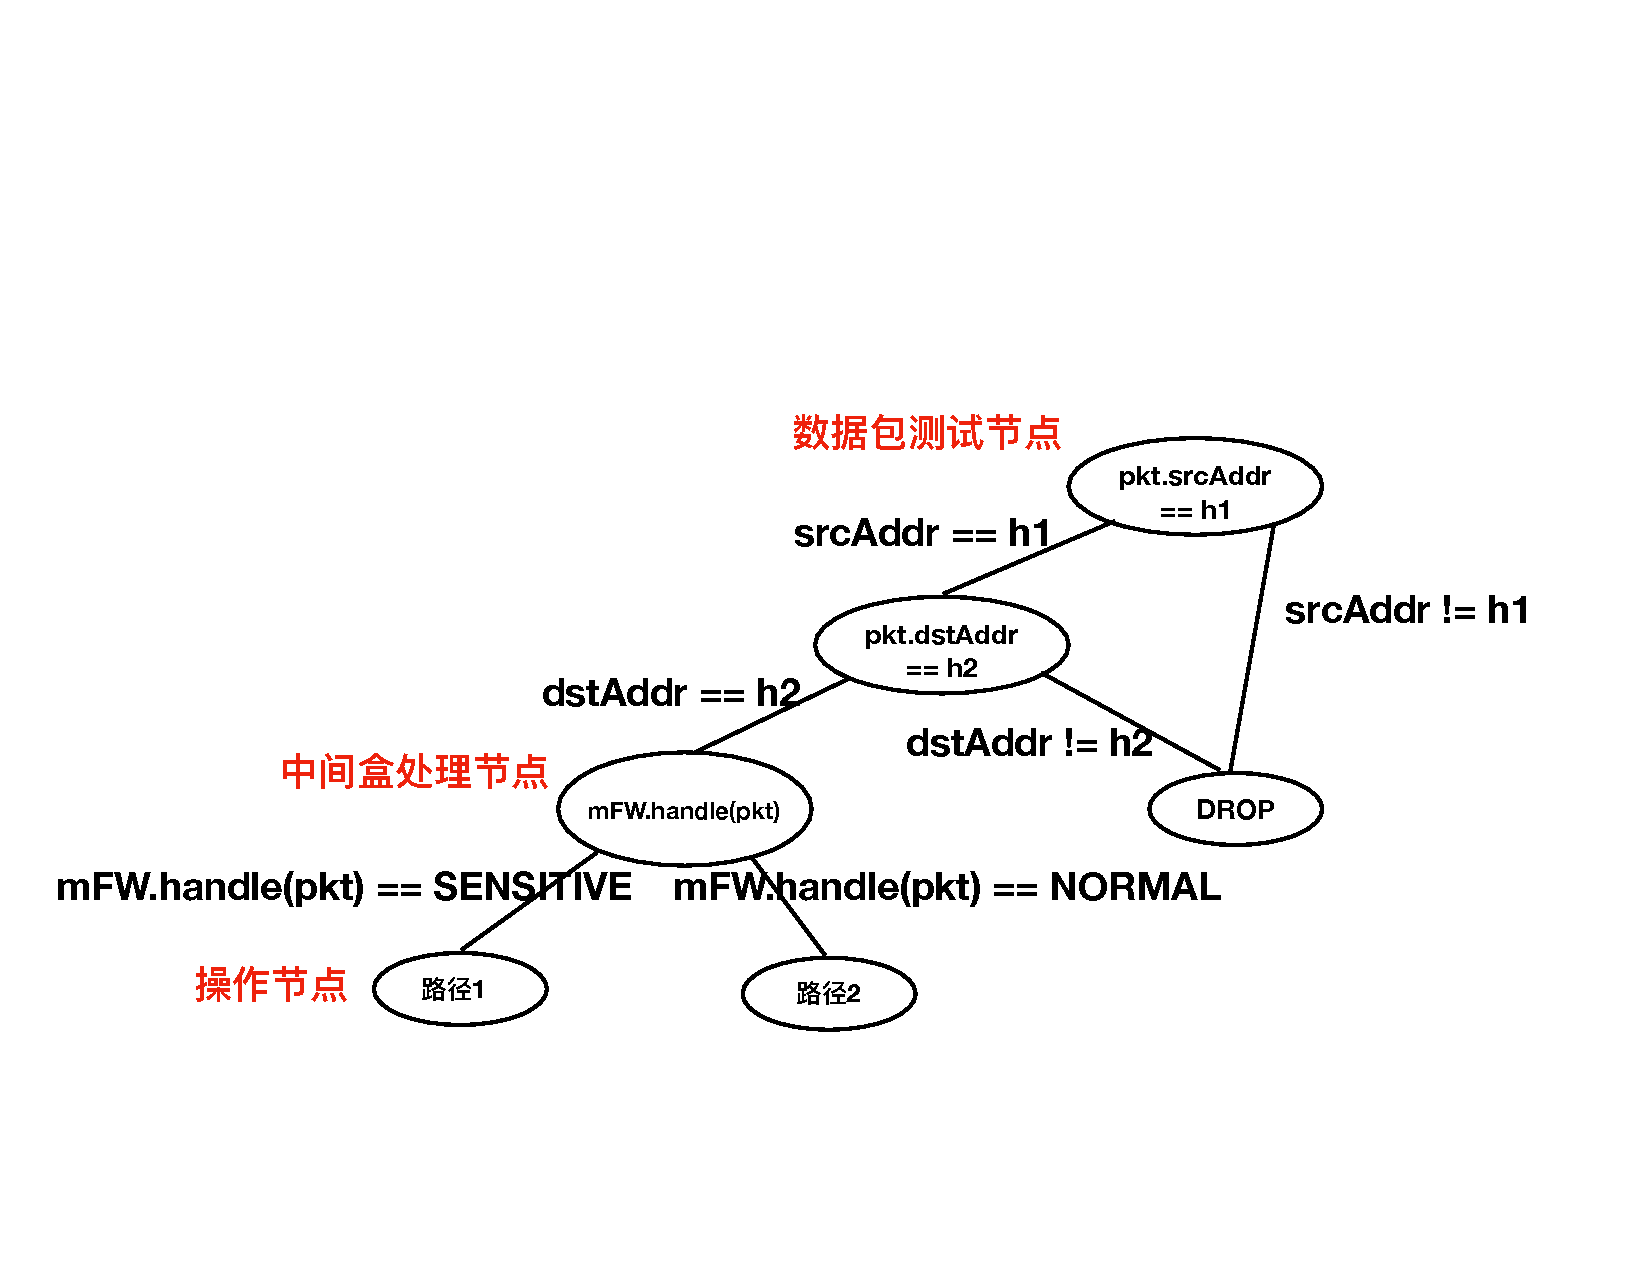
\includegraphics[width=\linewidth]{figures/ss-126.pdf}
\end{subfigure}
\vspace{-2mm}
\caption{\small Example of DG.}
%\vspace{-2mm}
\label{fig:dg-example}
\end{figure}

Given a DG, we denote the sequence of nodes and edges from the root to an action node (\ie, path constraint $pc$) as the trace of $pc$ ($T(pc)$). Then, given a trace $T(pc)$, we denote the middlebox-operation nodes of $T(pc)$ as $M(pc)$ (\ie, a sequence of nodes). As middlebox-operation nodes represent the packet handling of middleboxes, to not form loops, every middlebox-operation node can only appear once in $M(pc)$. Also, by extracting middlebox-operation nodes that represent stateful middleboxes from $M(pc)$, we have a subsequence of $M(pc)$ that every node is for stateful middlebox operations (denoted by $M^s(pc)$). Given a $T(pc)$, the SPC for its action node can be easily computed as the $T(pc)$ gives the trace of the packet enters the action node.

\vspace{-2mm}
\subsection{Path Computation}

As the leaf nodes in DG are path constraints, path computation targets to compute the concrete paths for these leaf nodes with a system performance objective. (And if leaves are concrete paths, the path computation just skips them.)

\para{Packet forwarding model}: Before path computation, we first give a packet forwarding model with DG in the network as the following. As shown in Fig.~\ref{fig:pfm-example}, given a path ($gw, a, b$) in the motivating example, logically we consider every switch in the path has the DG of the example program where $P$ indicates a packet-test node, $M$ indicates a middlebox-operation node, and $A$ indicates an action node. The $A$ node with red color represents the corresponding constraints for the path. The first packet of the flow (arriving at $gw$) starts to traverse the DG as the red line in the figure. When the packet meets a middlebox-operation node, it will be sent to the corresponding middlebox through the tunnel. After the processing, the middlebox will send the packet back and share its local state (\ie, by installing/modifying rules in the state table) for the flow with the corresponding middlebox-operation nodes (each node can be viewed as a pair of state table and match table) at switches along the path. (If the middlebox is stateful, then it does not set any state but makes the packet carry the state.) After the traversal of the DG (\ie, arriving at the leaf node along the red line), the packet will get the path and should be forwarded along the path. As local states have been shared with corresponding middlebox-operation nodes (or carried by the packet for stateful middleboxes) at other switches, the packet does not need to be sent to the middlebox again at the next switch. We denote a forwarding of a packet as stable forwarding if the packet does not access any stateless middlebox (compared with the first packet that should access them). Based on the stable forwarding, we can extend original SPC variable to \codeword{SPC.stable} which means the system path constraints only for stable forwarding paths (\ie, remove the stateless middleboxes). Then, to allow the state sharing, \codeword{SPC.stable} should be used as \codeword{SPC} includes the whole constraints for all packets including the first packet that must pass through all the middleboxes.

\begin{figure}[!htbp]
%\vspace{-2mm}
\centering
\begin{subfigure}{0.8\linewidth}
      \centering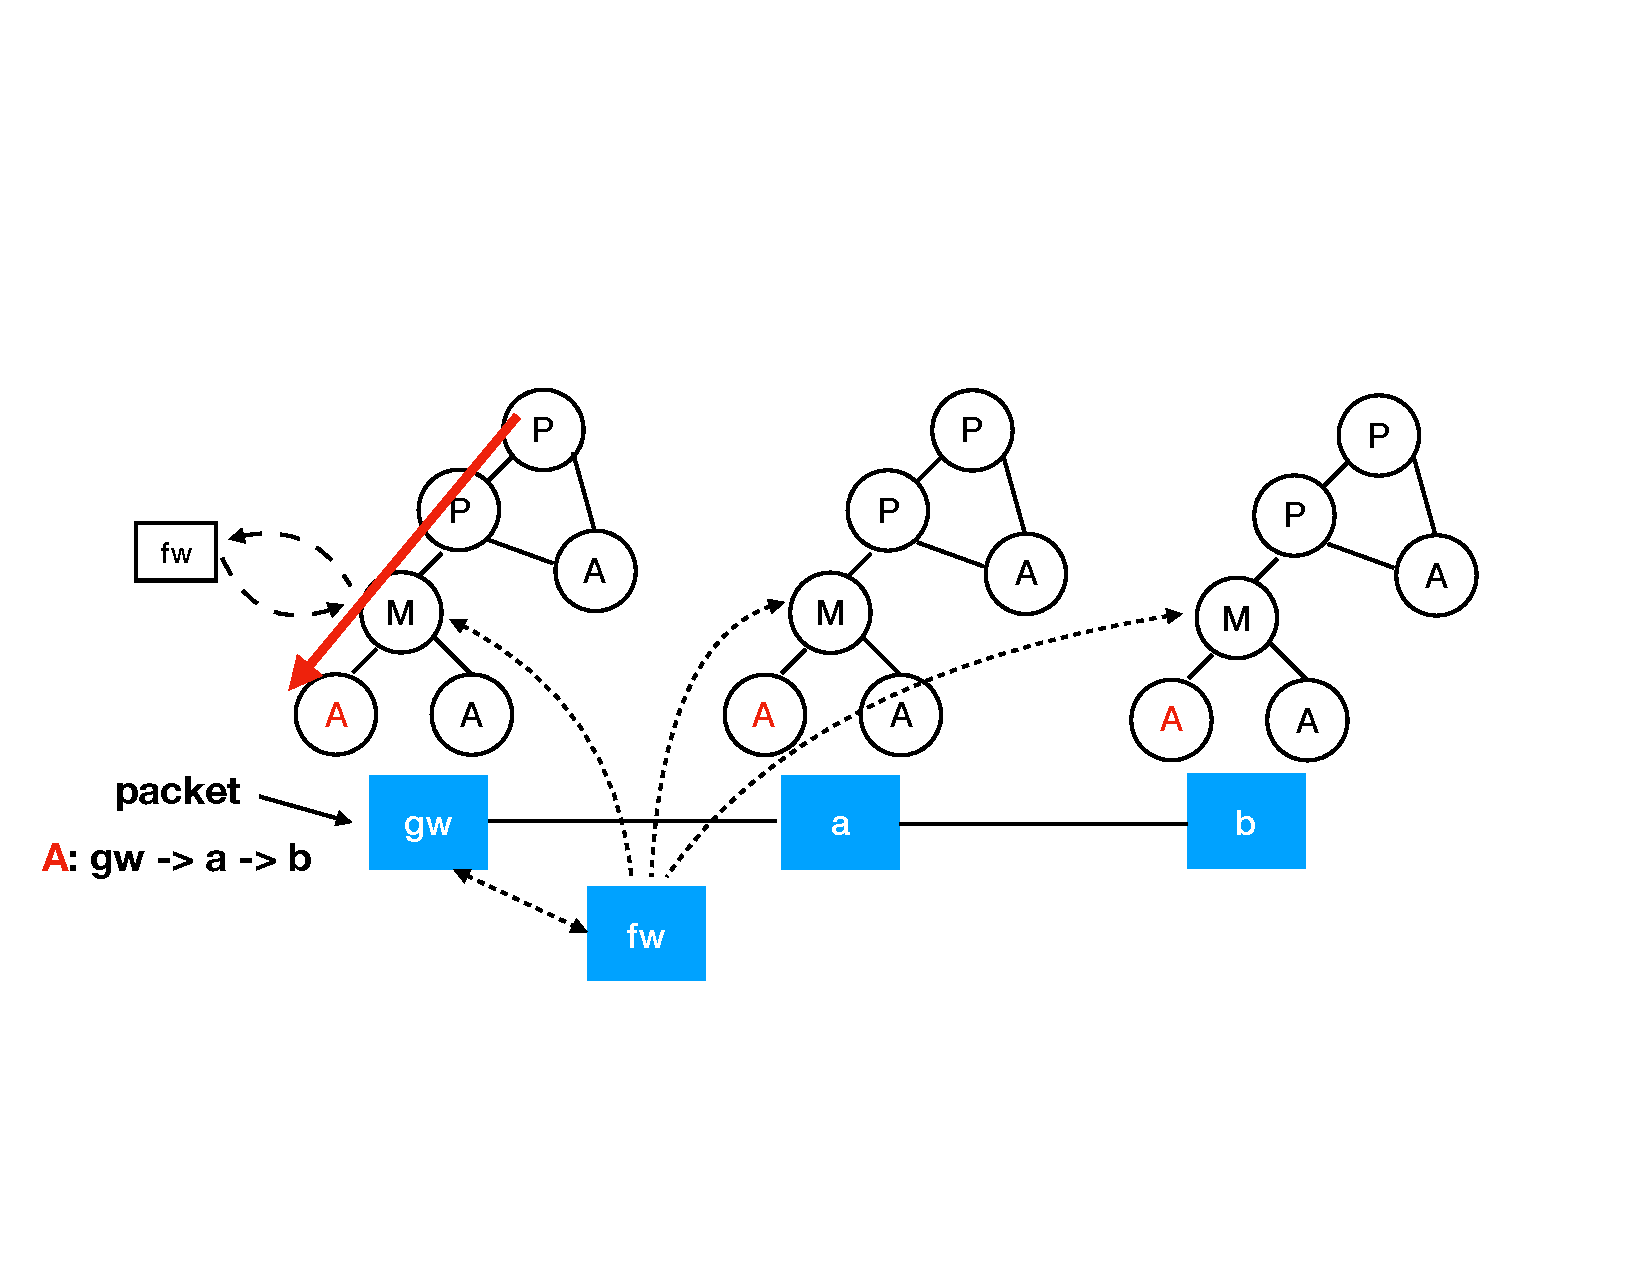
\includegraphics[width=\linewidth]{figures/ss-127.pdf}
\end{subfigure}
\vspace{-2mm}
\caption{\small Packet forwarding model with DG.}
%\vspace{-2mm}
\label{fig:pfm-example}
\end{figure}

%We denote the forwarding of the packets do not involve the stateless middleboxes as the stable forwarding.

%\para{Initialization for waypoints constraints}: As the initial process, for every action node in the DG, system should identify its source and destination nodes in the network. (This can be achieved by the hints from network operators as~\cite{arashloo2016snap}.) Then, add the source and destination nodes and also the $M^s(pc)$ to the corresponding waypoints constraint as the processing of stateful middleboxes should have a correct order. We consider the waypoints constraint as a set of node pairs where a pair has the form $(x, y)$ which indicates packets must pass through $x$ before $y$. (Note that $x$ and $y$ can be source/destination nodes.)

\para{System objective}: Based on the model, as the forwarding of the first few packets has little influence on the performance of the flow, a simple path computation (that only considers the stable forwarding) would be the following. We consider the objective of the network is to maximize the total throughput, \ie, maximize $\sum_ib_i$ where $i$ is the index of the path constraint $pc_i$ and $b_i$ is its throughput. The definition of variables can be found at Table~\ref{table:variables}. And the constraints can be found at Table~\ref{table:constraints} (where $Path(x, y, E)$ means there exists a simple path starting from $x$ to $y$ in $E$). In this paper we focus on the waypoints constraints for the path constraints (as they may complicate the path computation) and we consider the waypoints constraint as a set of node pairs where a pair has the form $(x, y)$ which indicates packets must pass through $x$ before $y$. (Note that $x$ and $y$ can be source/destination nodes.)

\begin{table}[]
\scriptsize
\begin{tabular}{l|l}
Variable     & Description                                                             \\ \hline
$u_i$, $v_i$ & The source and destination nodes of path constraint $pc_i$                            \\ 
$E$          & All edges (an edge $e$: $(e.src, e.dst)$) in the network                       \\
$m_e$        & The maximum bandwidth of $e$                                            \\
$W_i$        & A set of node pairs of $pc_i$ \\
$z^i_e$      & The edge $e$ is selected by $pc_i$ \\
$b_i$          & The bandwidth of flows using the path for $pc_i$                                   
\end{tabular}
\caption{\small Notation.}
\label{table:variables}
\end{table}

\begin{table}[]
\scriptsize
\begin{tabular}{l|l}
Constraint                                        & Description                               \\ \hline
$\forall i, \forall (x, y) \in W_i, Path(x, y, E)$                    & Path constraints                  \\
$\forall i, Path(u_i, v_i, E)$      & Path exists in $E$     \\
$\forall e \in E, \sum_ib_i*z^i_e \le m_e$   & Bandwidth constraints for edges
\end{tabular}
\caption{\small Constraints.}
\label{table:constraints}
\end{table}

As the system path constraints have been added into the path constraints (by using the \codeword{SPC.stable}), the correctness can be guaranteed. And it enforces a packet must get results of stateful middleboxes and then select the correct path.

%However, this simple solution can get optimal paths only if all the middleboxes are stateless. If there is a stateful middlebox, the constraints of stable forwarding should not only consider the waypoints constraints specified by the program as it also must pass through the stateful middleboxes.
%
%Then, people may add another constraint as the following: $\forall (x, y) \in M^s(pc_i), Path(x, y, E)$. This constraint enforces that the optimal paths must pass through all the stateful middleboxes in a correct order (\ie, $M^s(pc_i)$). This seems correct as now the stable forwarding includes the stateful middleboxes. 
%
%However, this is not enough. Considering the example as shown in Fig.~\ref{fig:c-example}. As the middlebox $M$ is stateful, the new added constraint enforces that the computed optimal paths should pass through $M$. However, the result could be that $M$ is behind the branch of waypoints $b$ and $c$. In this case, when a packet arrives at $a$, it cannot decide how to forward to $M$ as which path to select depends on the result of $M$.
%
%\begin{figure}[!htbp]
%%\vspace{-2mm}
%\centering
%\begin{subfigure}{0.9\linewidth}
%      \centering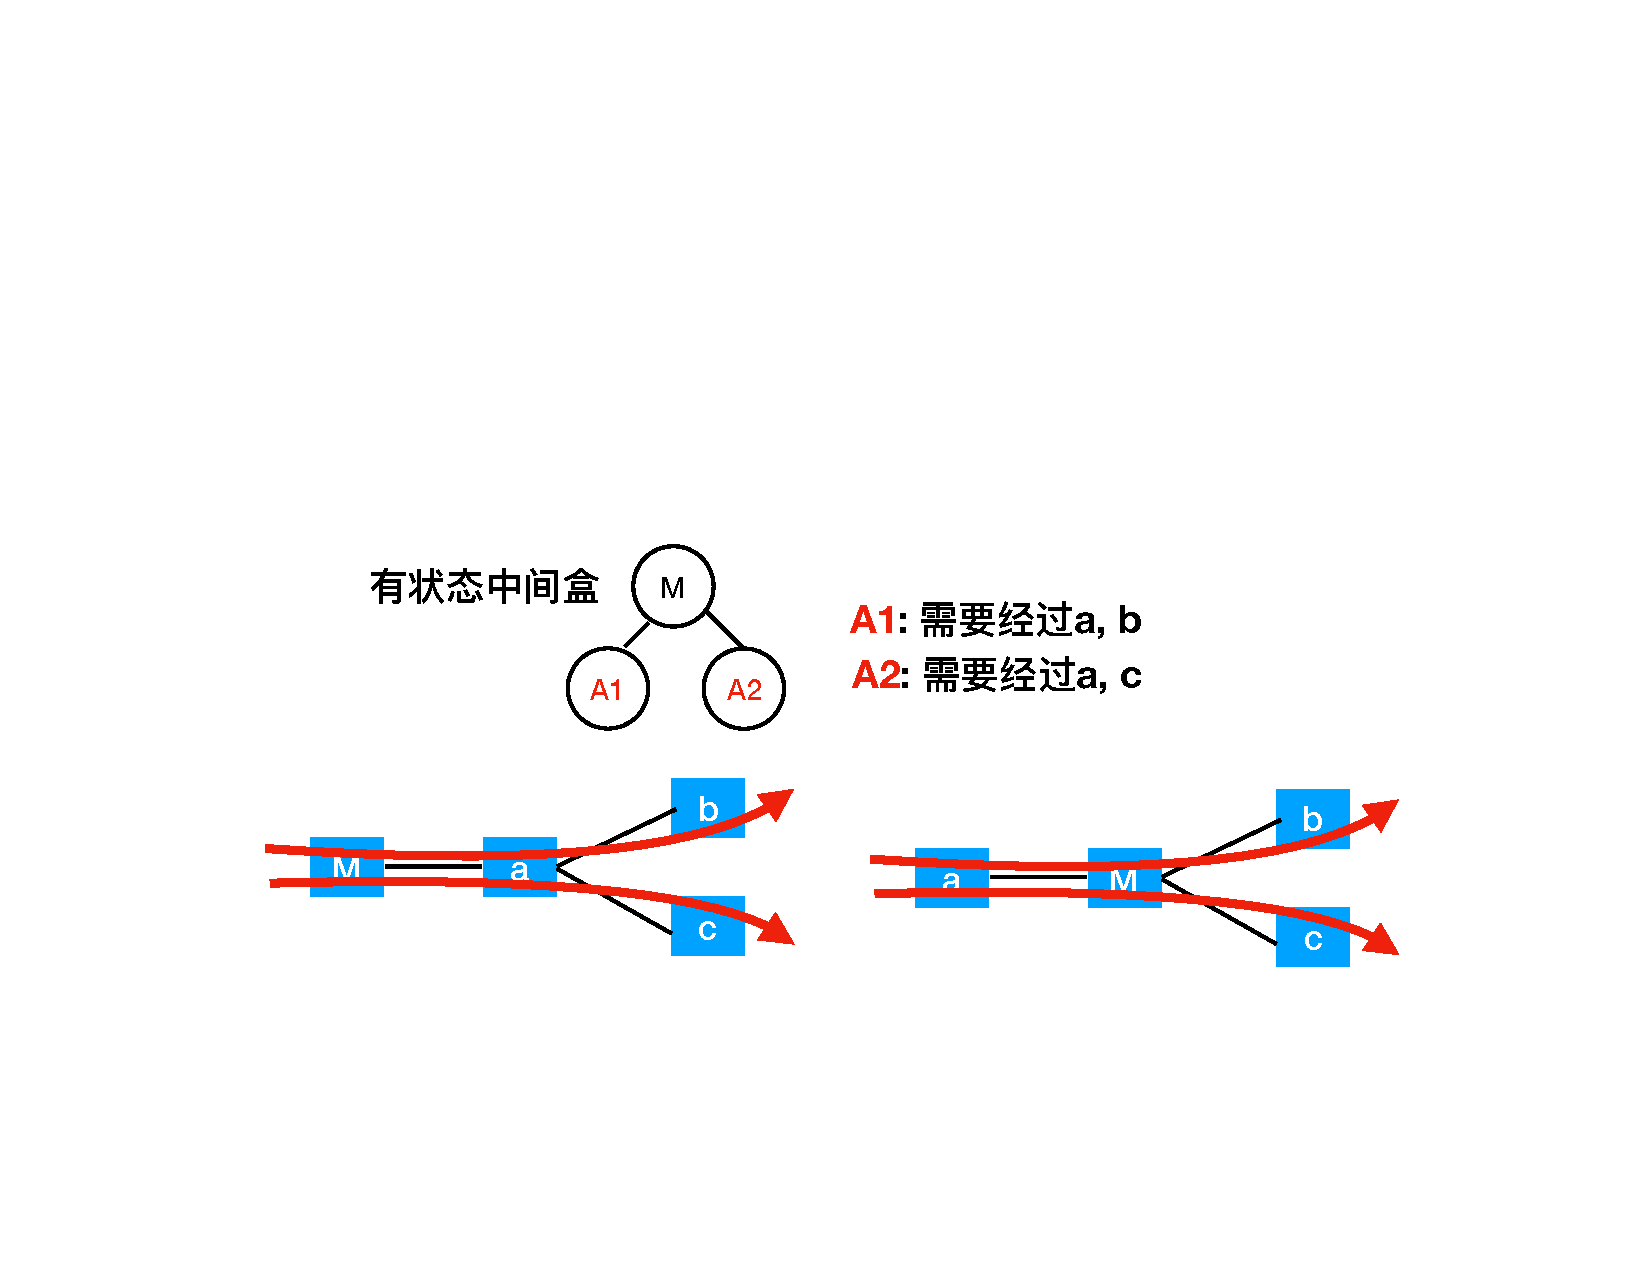
\includegraphics[width=\linewidth]{figures/ss-128.pdf}
%\end{subfigure}
%\vspace{-2mm}
%\caption{\small An example to show that the dependencies between middlebox-operation nodes and waypoints should be considered.}
%%\vspace{-2mm}
%\label{fig:c-example}
%\end{figure}
%
%To resolve the issue in Fig.~\ref{fig:c-example}, one solution is to add constraints $(M, b)$ and $(M, c)$ to  $A_1$ and $A_2$ respectively. Then the paths in Fig.~\ref{fig:c-example} cannot exist as they does not satisfy the constraints. The idea is to enforce a packet must get results of stateful middleboxes and then select the correct path.

However, the current path constraints may cause \emph{excessive constraints} for paths. For example, a stateful middlebox-operation node ($M$) has two path constraints $A_1$ and $A_2$ as its children in a DG. And, $A_1$ specifies a path must pass through switches $s_1, s_2$; $A_2$ specifies a path must pass through switches $s_1, s_3$. Then, the path constraints have $(M, s_1)$ for both $A_1$ and $A_2$ as it simply connects the waypoints constraint in \codeword{SPC.stable} and $s_1, s_2$ (also $s_1, s_3$). However, this is only a sufficient condition as some other conforming paths are excluded (\eg, $s_1 \rightarrow M \rightarrow s_2\ (s_3)$).

\para{Waypoints constraints computation}: Instead of simply connecting two waypoints constraints, now we give an algorithm to compute the waypoints constraints that enforces all the paths are correct and no conforming paths can be excluded. The high-level structure of the algorithm is to do a depth-first traversal for a DG. The traversal only considers the stateful middlebox-operation nodes and action nodes (and traverses a stateful middle operation node only after all its children are finished). When traversing a stateful middlebox-operation node, we can get all possible waypoints constraints under its decision. Then, the processing of the node is to update these constraints (each of which can be modeled as a directed acyclic graph, DAG). As discussed before, we do not want to add excessive constraints. And the solution is simple: When processing a middlebox node $M$, if all the no-incoming-edge nodes of $M$'s possible constraints (\ie, DAGs) are the same, then skip these nodes recursively until these nodes are not the same and then add edges ($M$, $x$) to each of DAGs where $x$ is the node of the location that the skipping process stopped at. The insight is that, skipping a node is safe if and only if the node is the next waypoint node for \emph{all} the possible paths. For the example in Fig.~\ref{fig:skip}, the node $M$ has four possible path constraints (DAGs) and $a$ should be skipped when updating them.

\begin{figure}[!htbp]
%\vspace{-2mm}
\centering
\begin{subfigure}{0.8\linewidth}
      \centering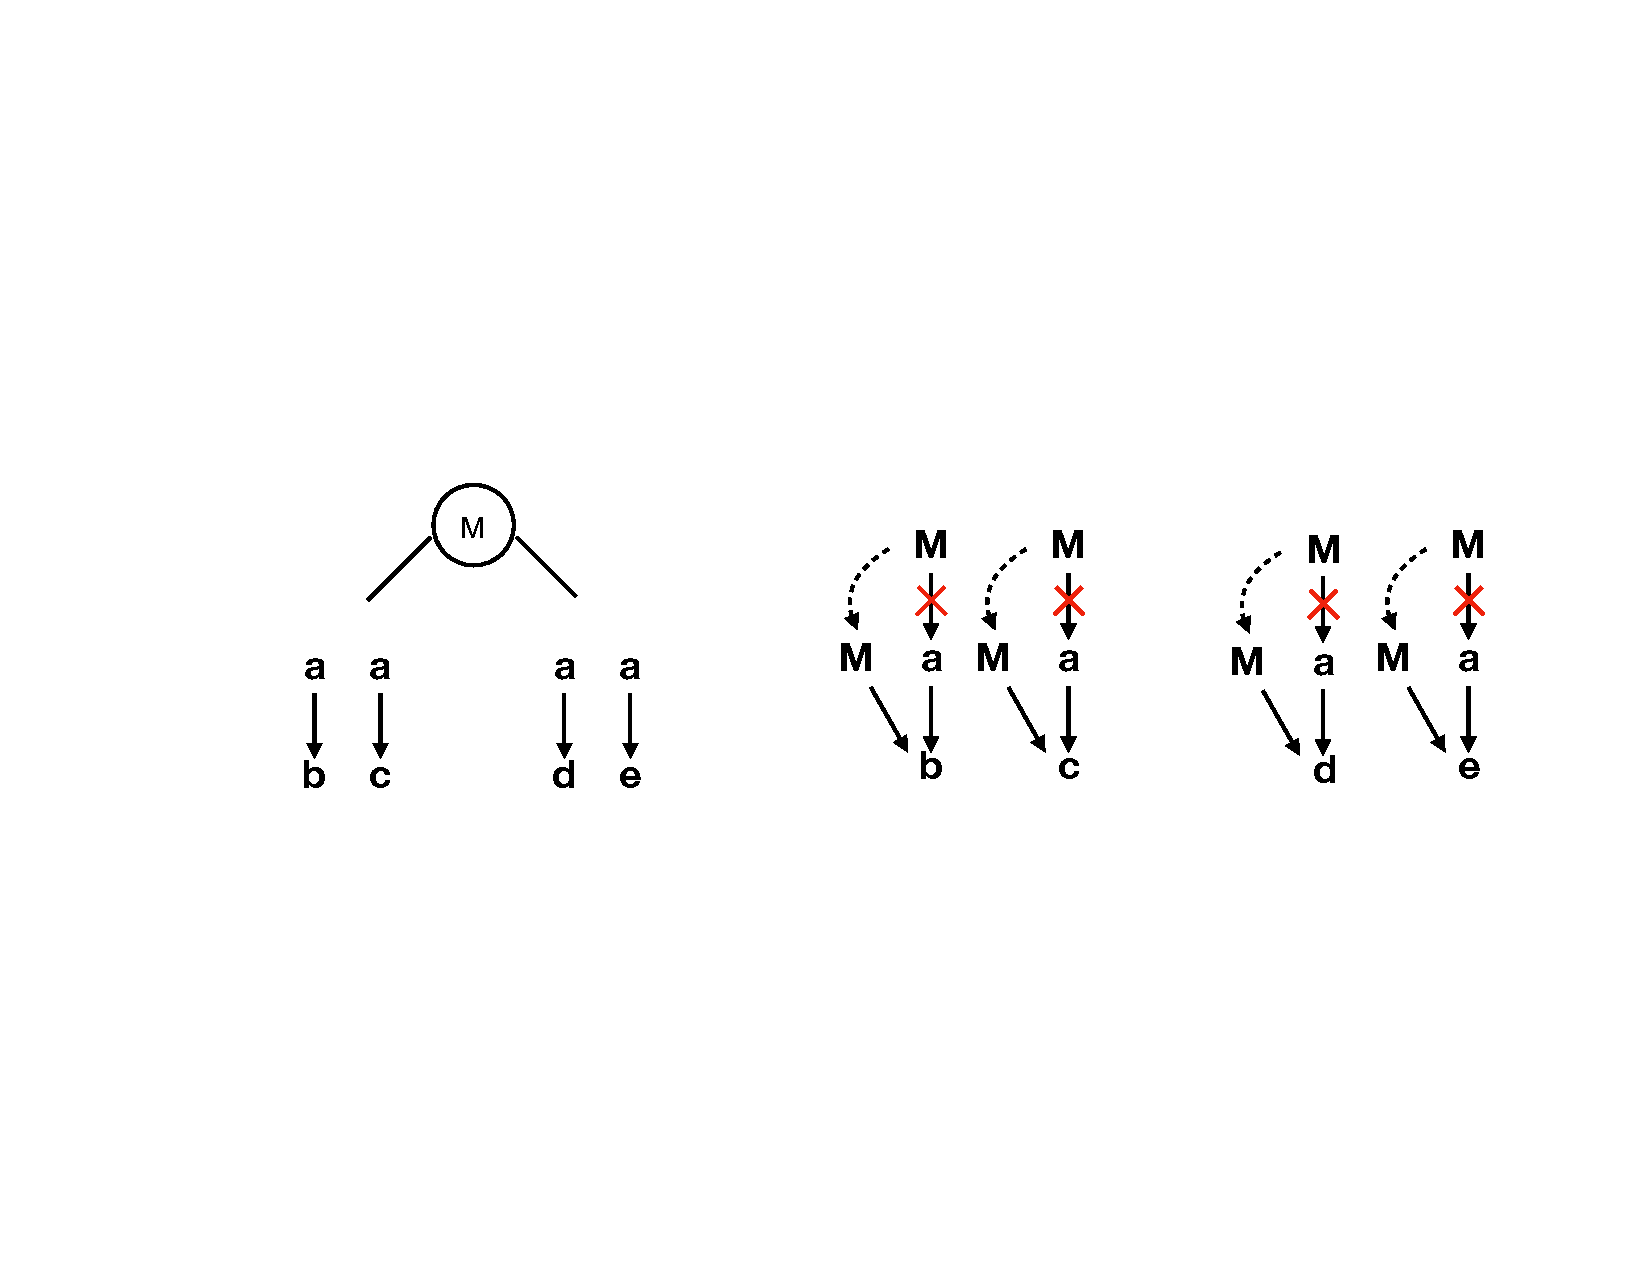
\includegraphics[width=\linewidth]{figures/ss-129.pdf}
\end{subfigure}
\vspace{-2mm}
\caption{\small Skip the same nodes.}
%\vspace{-1mm}
\label{fig:skip}
\end{figure}



%
%Based on the idea, we give an algorithm to solve the issue for general cases. The high-level   
%
%
%First, given a middlebox operation node $m$ in a DG, we denote a set of topology ordered waypoints constraints that $m$ can reach to in DG as $R(m)$. Also $R(m)$ can be partitioned by the out-edges of $m$, \ie, the out-edge $m^o_i$ has a subset of $R(m)$ (denoted by $R^i(m)$). If there is a stateful middlebox node $n$ in $R^i(m)$ that $m \rightarrow n \in M^s(p_i)$, then add $m \rightarrow n$ to $R^i(m)$. Given the new $R^i(m)$, we denote a set of nodes in $R^i(m)$ that has no order with $m$ as free nodes with $m$ in $R^i(m)$. Then, we extract the subgraph from $R^i(m)$ that only includes these free nodes into a new graph: $Free(R^i(m))$. Then, for all the $Free(R^i(m))$, if there exists $Free(R^i(m))$ is not equal to $Free(R^j(m))$, it means the result of $m$ is required to choose which out-edge to go. Therefore, the following constraints are need. For all the $Free(R^i(m))$, skip the same no-incoming-edge nodes recursively until it does not exist, and add the constraints: $m \rightarrow nexts(Free(R^i(m)))$ where $nexts(Free(R^i(m)))$ is the set of no-incoming-edge nodes after the skipping. Finally, for all stateful middlebox operation nodes, do the previous processing. For example, for the DG in Figure 6 (XXX), $M_2$ adds new constraints: $M_2 \rightarrow b$ and $M_2 \rightarrow c$ for $A_1$ and $A_2$. (Similar for $M_3$.) And then $M_1$ adds $M_1 \rightarrow M_2 (M_3)$.

\vspace{-2mm}
\subsection{Datapath Generation}

\para{Remove redundant nodes of DG}: After the path computation, there are concrete paths for all the leaf nodes in DG. We follow the packet forwarding model described previously that all the switches in the network have the same DG. It is easy to observe that if a switch does not belong to a path, then the corresponding leaf node of the path can be removed (and then the no-out-edge internal nodes). Also, by converting the path in a leaf node to the next hop in the network, we may still remove redundant nodes. Still consider the firewall example. After we convert the paths to next hops, we find that the two leaf nodes of the middlebox node are the same, \ie, switch $a$ in the network. This means the middlebox-operation node has no meaning for the gateway $gw$ since whatever the result of the node is, the next hop does not change. Therefore, we can remove the node and replace with the leaf node with the next hop $a$. Fig.~\ref{fig:rv} illustrates the process. 

Then, for the switch side, based on the updated DG, it can generate tables and flow rules easily with the multi-table pipeline structure. Note that a middlebox-operation node can be viewed as a state table following a match table. As for the middlebox side, if it is a stateless middlebox, then for the datapath it only needs to care about is switch-middlebox tunnels which also can be easily generated. For the stateful middleboxes, as they belong to computed paths, they can be viewed as switch nodes with stateful functions that can embed the results to the packets. When a packet meets a stateful middlebox node in DG of a switch, and the node cannot be replaced with a leaf node, then any next hop under the node is acceptable since it must eventually arrive at the middlebox and any path from the switch to the middlebox must follow the path constraints.

\begin{figure}[!htbp]
%\vspace{-2mm}
\centering
\begin{subfigure}{0.8\linewidth}
      \centering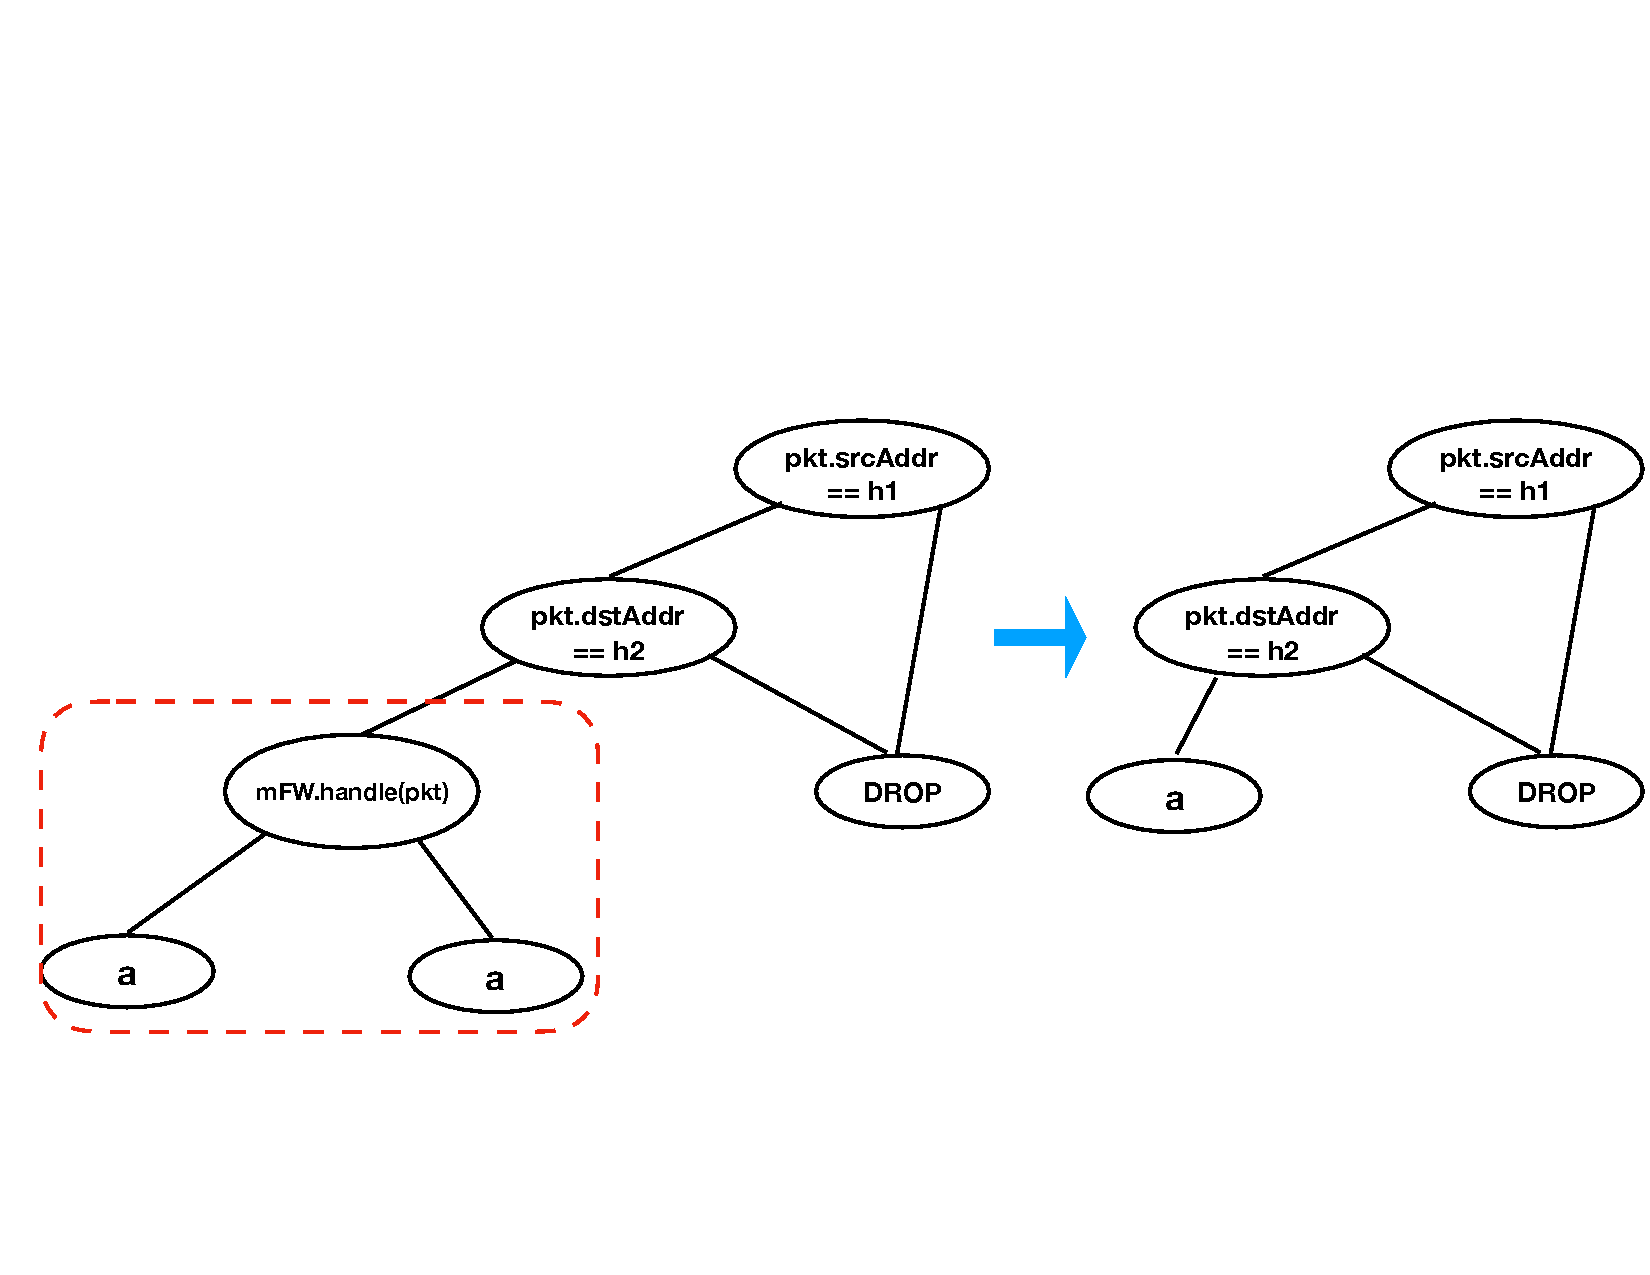
\includegraphics[width=\linewidth]{figures/ss-130.pdf}
\end{subfigure}
\vspace{-2mm}
\caption{\small Remove redundant middlebox nodes.}
%\vspace{-2mm}
\label{fig:rv}
\end{figure}

\para{Order of messages}: The next issue is how a stateless middlebox share local states (\ie, update states) in other switches. It needs to guarantee that for any targeting switch, the update message should arrive earlier than the packet. For example, in the firewall example, only the step 2 is finished, step 3 can be executed. Then a simple solution can be making the packet carry the update message. Different with the state carrying for stateful middleboxes, this message can install/modify rules in the state table of the corresponding middlebox-operation node.





%In this section, we will discuss the implementation of the general network-wide stateful packet processing to provide a more flexible state updates. First, we will show the consistency problem in the general network-wide stateful packet processing. Then, we will present two techniques for the problem.
%
%\subsection{Consistency problem}
%
%As discussed in Sec. 2, the consistency requirement demands a packet must see the newest states which may be updated by the previous packet. Let us consider the example shown in Figure. 3 with two switches $sw_1$ and $sw_2$ and two maps $m_a$ and $m_b$ are stored in the two switches respectively. Now a flow with packets $pkt_1, pkt_2, ..., pkt_i, ...$ try to be processed with three operations: read $m_a$; read $m_b$; write $m_a$. Then, the problem arises that when $pkt_i$ tries to read $m_a$, how to guarantee that $pkt_i$ reads the updated value of $m_a$?
%
%%figure 3
%\begin{figure}[!htbp]
%%\vspace{-2mm}
%\centering
%\begin{subfigure}{0.7\linewidth}
%      \centering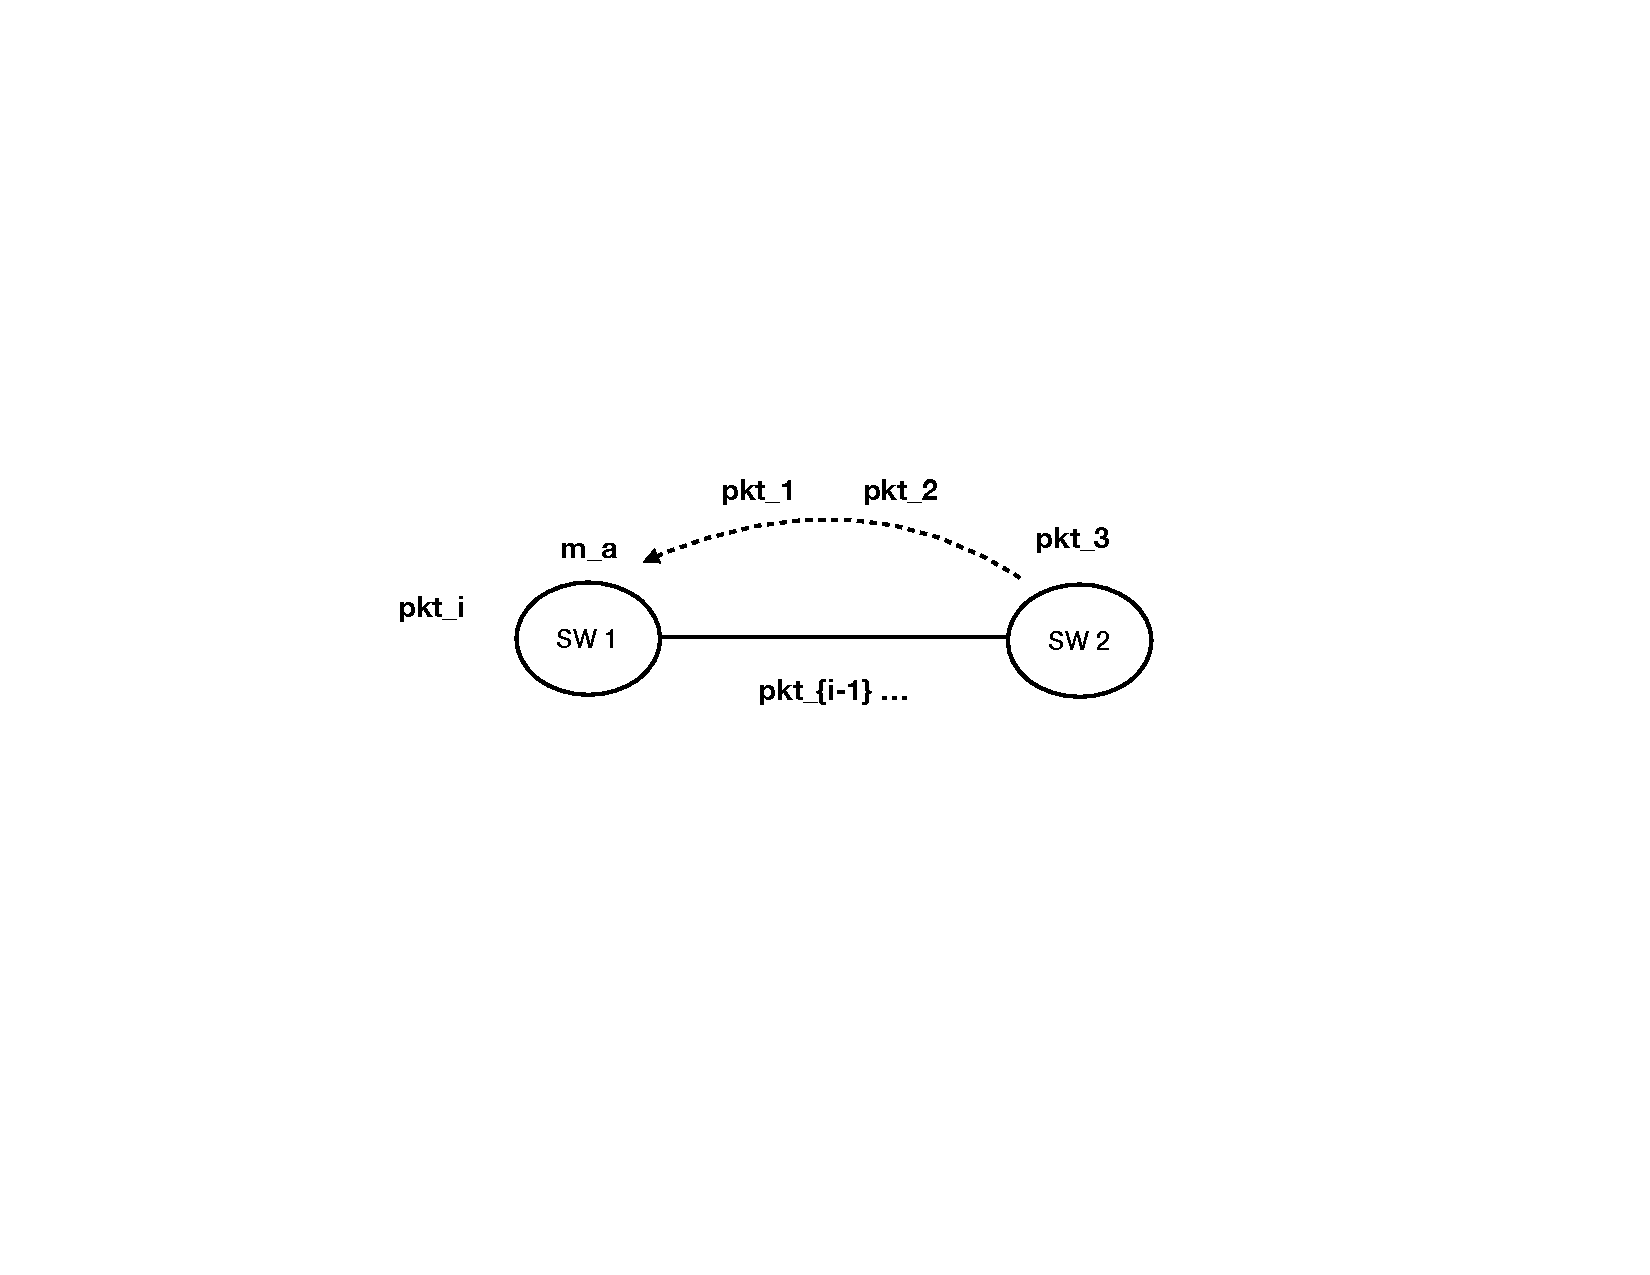
\includegraphics[width=\linewidth]{figures/69.pdf}
%\end{subfigure}
%%\vspace{-2mm}
%%\caption{\footnotesize{The CDF of job latency local and remote jobs.}}
%\caption{\small Example of two switches.}
%%\vspace{-2mm}
%\label{fig:mtv-example}
%\end{figure}
%
%A naive solution to the problem is to let every packet wait until the previous packet has updated the state. But there are two issues: one is how the packet knows the state has been updated (the previous packet may not update the state); two is that the waiting packets in the switch not only causes the latency issue but only occupies the queue storage in the switch. In the following subsections, we will show two techniques to solve the problem.
%
%\subsection{Fixed-route packets}
%
%Consider the Figure 3, when $pkt_i$ arrives at $sw_1$ trying to access $m_a$, the first thing $pkt_i$ needs to check is that whether there are previous packets trying to update $m_a$. As the waiting approach may cause serious performance issue, a new design is needed.
%
%As the constraint that there is only one loop for a flow to access a state variable (discussed in the target paragraph), if there are any packets (in the same flow with $pkt_i$) trying to update $m_a$, these packets should be in the loop. Then, if $pkt_i$ can pass through the loop (without causing any updates to any state), when $pkt_i$ arrives $sw_1$ again, it can make sure that all the previous packets (if any) have finished the updates. This can be achieved by adding a special tag (Fixed-Route, FR) to $pkt_i$. When $pkt_i$ tries to access $m_a$, $pkt_i$ should first be tagged with $FR_a$ specifying the packet $pkt_i$ is trying to access $m_a$. Then, the FR $pkt_i$ is forwarded to the corresponding loop of $m_k$. When $pkt_i$ with the FR tag arrives at $sw_1$ after passing through the loop, it should first remove the FR tag from $pkt_i$ and then $pkt_i$ can access $m_a$ with any operations.
%
%\begin{figure}[!htbp]
%%\vspace{-2mm}
%\centering
%\begin{subfigure}{0.7\linewidth}
%      \centering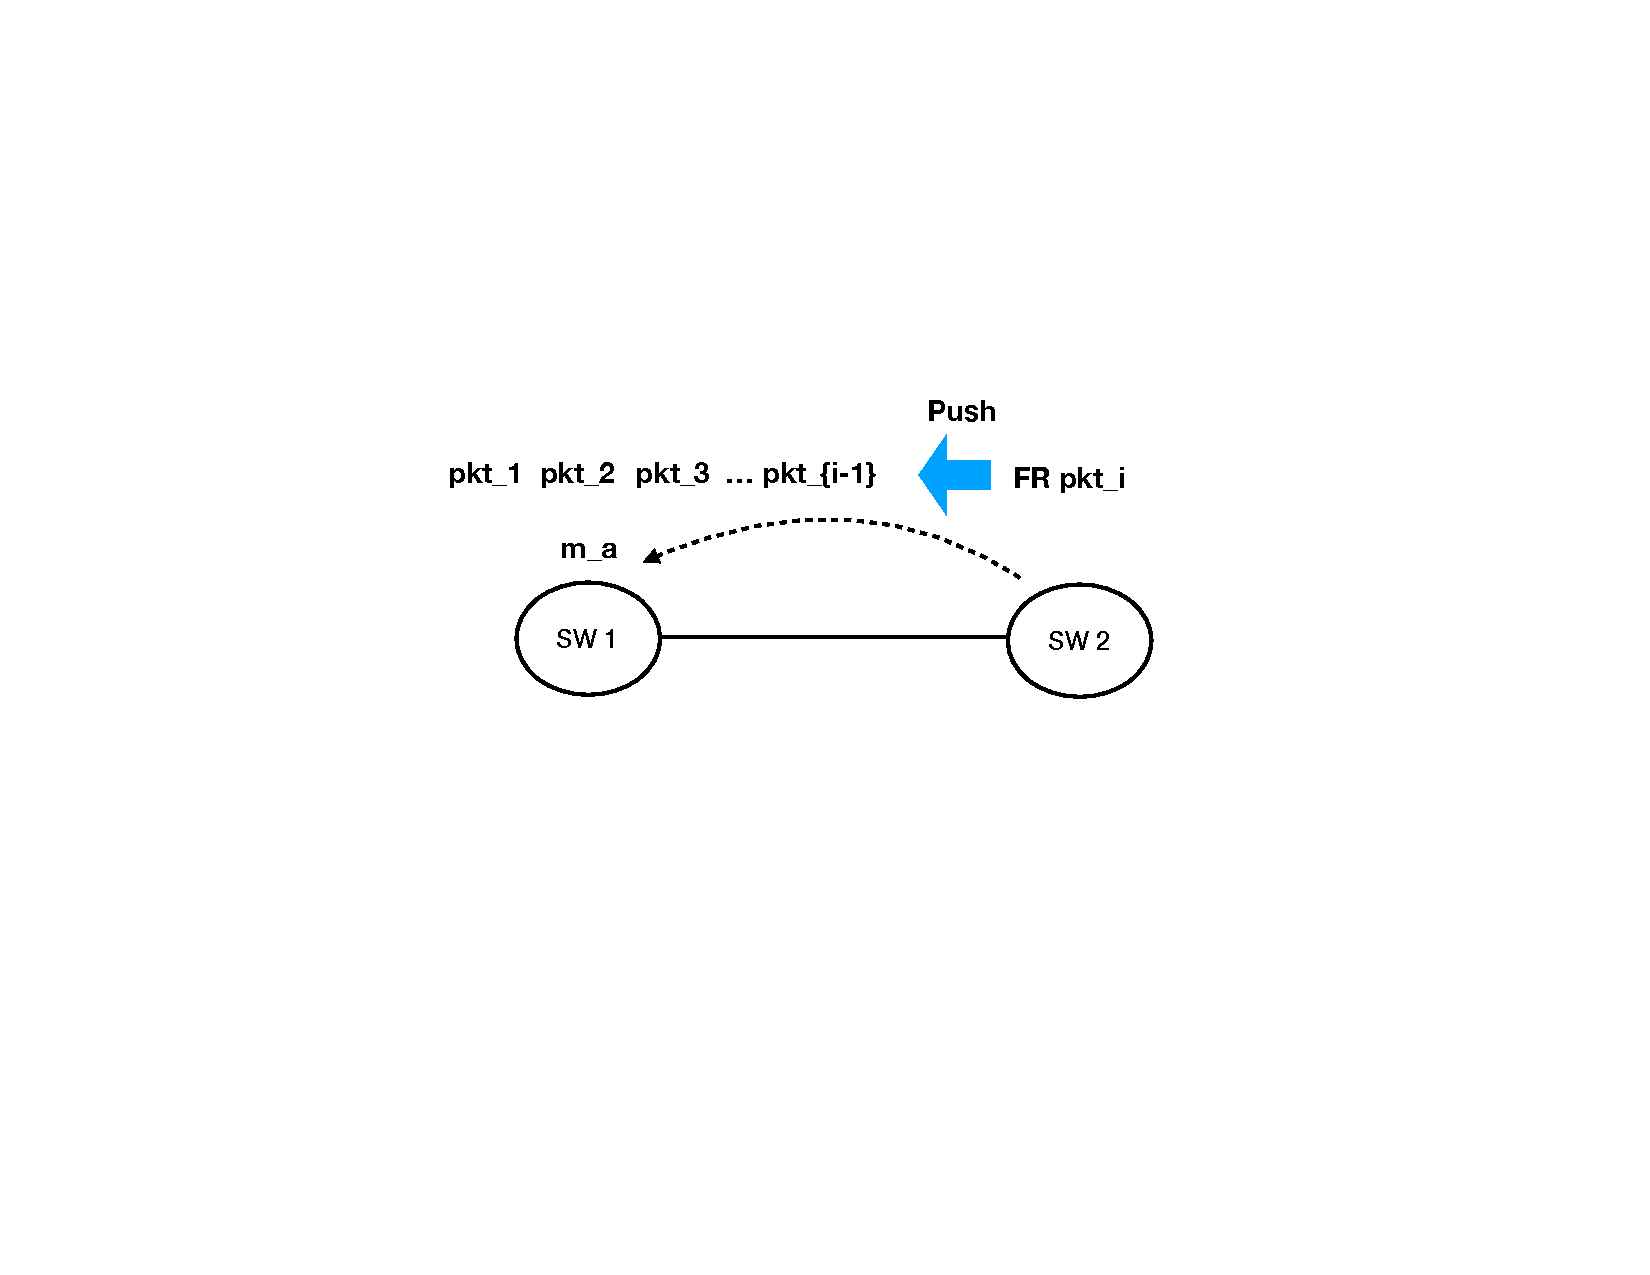
\includegraphics[width=\linewidth]{figures/70.pdf}
%\end{subfigure}
%%\vspace{-2mm}
%%\caption{\footnotesize{The CDF of job latency local and remote jobs.}}
%\caption{\small Example of FR packets push the previous packets.}
%%\vspace{-2mm}
%\label{fig:mtv-example}
%\end{figure}
%
%The intuition is that the FR packet will ``push out'' all the potential previous packets that may update $m_a$ in the loop.Therefore, whenever the FR packet arrives $sw_1$, it can make sure that all the previous updates have been applied. However, one issue of the FR tag design is that it seems \emph{all} packets should experience the loop which may cause potential latency.
%
%%
%%
%%\subsection{Two-version states}
%%
%%First, to not let packets wait in the switch, a simple solution is to forward packets. As the consistency requirement is for packets belong to the same flow with the same path (TODO), if no state updated, a packet should follow the same path as the previous packet does. Now the problem is how to make the packet see the updated state.
%%
%%The solution is to maintain two versions of states: one is for the new incoming packets; the other is for the packets arriving twice. Specifically, given a state $m_k$ stored in switch $sw_k$, we maintain two versions of $m_k^{old}$ and $m_k^{new}$. In the beginning, $m_k^{old}$ keeps the original value of $m_k$ and $m_k^{new}$ is null. When a new incoming packet $pkt_i$ arriving at $sw_k$ tries to read $m_k$, as this is the first time $pkt_i$ reads $m_k$, the result is the value of $m_k^{old}$. Over a period of time, $pkt_i$ arrives $sw_k$ again and tries to write a value to $m_k$. Then, the updated value is stored in $m_k^{new}$. Now consider another packet $pkt_{i+1}$ following $pkt_i$ arrives at $sw_k$. Packet $pkt_{i+1}$ tries to read $m_k$ and it returns the value of $m_k^{old}$ which leads $pkt_{i+1}$ to follow the same path of $pkt_i$. When $pkt_{i+1}$ arrives at $sw_k$ again, it realizes that the value of $m_k$ has been updated (as the value is not null), then it reads the updated value from $m_k^{new}$. At this point, it achieves that $pkt_{i+1}$ sees the updated value of $m_k$. Table XXX shows which version of $m_k$ should be considered with different cases. Note that first arrival means that the packets is the new incoming and second arrival means that it is the second time the packet arrives at $sw_k$.
%%
%%\begin{table}[]
%%\begin{tabular}{|l|l|l|l|l|}
%%\hline
%%\multirow{2}{*}{} & \multicolumn{2}{l|}{$m_k^{new}$ == null} & \multicolumn{2}{l|}{$m_k^{new}$ != null} \\ \cline{2-5} 
%%                  & Read from           & Write to           & Read from           & Write to           \\ \hline
%%First arrival                & $m_k^{old}$         & $m_k^{old}$        & $m_k^{old}$         & $m_k^{old}$        \\ \hline
%%Second arrival                & $m_k^{old}$         & $m_k^{new}$        & $m_k^{new}$         & $m_k^{new}$        \\ \hline
%%\end{tabular}
%%\end{table}
%%
%%To make a packet knows that whether it is the second time to arrive at a switch and try to access (including read/write) a state variable at the switch, a simple but useful approach is to embed the historical accesses of state variables to the packet. When a packet tries to access a state variable, it first needs to check the historical accesses of state variables to see whether the state variable has been accessed before. After the checking, it can decide which version of the state should be read from/written to.
%%
%%The insight of the two-version design is that whenever a packet arrives a switch and tries to access a state, it can realize two things: one is that whether this is the first arrival or the second arrival; two is that whether the state has been updated or not. If it is the second arrival and the state has been updated, then for the consistency requirement, the packet must be processed as if it is the \textbf{first} time the packet tries to access the state. (Note that in this case, the exceeding part of the historical accesses of state variables also should be deleted.) Then, the consistency is guaranteed as the packet has seen the updated state.
%%
%%\subsection{Multi-version states}
%%
%
%
%\subsection{Counter and timer to break loop}
%
%The issue of the FR tag design is that a packet \emph{always} first be tagged with FR and pass through the loop, and then the packet can be processed with normal operations. In this section, we will show how to use a counter and a timer to break the loop easily.
%
%%the old version of a state even the state has been updated, which may cause a ``redundant'' loop of state accesses that increases the latency.
%
%For each state variable $m_k$, it has a counter $c_k$ to record the current number of FR packets (with $FR_k$) in the corresponding loop of $m_k$ that try to update $m_k$. Specifically, when a packet is tagged with $FR_k$, the counter $c_k$ increases one to indicate there is a new packet entering $m_k$'s corresponding loop. When a FR packet with $FR_k$ finish the loop and arrive the switch of $m_k$, the counter $c_k$ decreases one to indicate there is a packet removed from the loop. Then, the counter $c_k$ is able to give the current number of packets in the loop.
%
%As the TCP packets enter the network in a burst way (for UDP packets, as there is no order among them, the consistency requirement is not important), if the interval time between two bursts of packets is large enough, the packets in the loop can be all pushed out indicated by the value of counter equals to zero. Fortunately, as the burstiness of TCP is at RTT and subRTT scale [ref: XXX], and the loop latency in data planes should be much smaller than that [ref: XXX], for every first packet of bursts of packets trying to access $m_k$, the counter $c_k$ has a high possibility to be zero.
% 
%When the counter of $m_k$ becomes zero, any packet can access $m_k$ immediately without tagged with $FR_k$ as there is no packet in the loop trying to update $m_k$. However, when a packet accesses $m_k$, the packet can either access $m_k$ or not, which cannot be determined. Therefore, it cannot make sure whether the packet is in the loop or not.
%
%Here we introduce a timer $t_k$ for $m_k$. The timer $t_k$ records the time of the last packet without FR tag that accesses $m_k$ and leaves the switch. When a new packet arriving at the switch and trying to access $m_k$, if the counter $c_k$ is zero, then compute the time: $current\_time - t_k$. If the computed time is larger than the time $t_x$ where $t_x$ is larger than the latency time of the corresponding loop of $m_k$, it is very likely that the previous packet does not enter the loop. Then, the new packet can access $m_k$ and leaves the switch (also update the value of the timer $t_k$). As the loop is fixed, by choosing the value of $t_x$, the error rate can be reduced to packet loss rate. Also the computation of the latency of the corresponding loop of $m_k$ can be easily achieved as it can sample several FR packets passing through the loop and compute the average latency for these FR packets. However, if the computed time is smaller than the time $t_x$, then the packet should be tagged with FR and forwarded to the loop which has been discussed in previous subsection.
%
%%
%%A naive solution to break the loop is that when the state is updated (\ie, the new version of the state is not null), the packet accesses the new version of the state. However, this solution is wrong: the new version of the state can be updated multiple times. It cannot guarantee that all the previous updates have been applied to the state when a packet try to access the state.
%%
%%The solution to that issue is to set a timer to a state to record the time that the last packet accesses the old version of the state. Specifically, given a state $m_k$ at switch $sw_k$, a timer $t_k$ is set to record the time that last packet $pkt_i$ access $m_k^{old}$. We denote that time as $t_k^i$. When another packet $pkt_{i+1}$ arrives at the switch and tries to access $m_k$, we compute the following interval time: $current\_time - t_k^i$. If the interval time is larger than a time $t_x$ where $t_x$ is larger than the time from $pkt_i$ sent from $sw_k$ to $pkt_i$ received again at $sw_k$ (denote as the loop time of $m_k$, \ie, LT($m_k$)), then $pkt_{i+1}$ can access the new version of $m_k$, which breaks the loop. As the state variables are already placed on the switches as well as the paths of packet processing, the computation of LT($m_k$) can be easily achieved by sending a prove packet along the corresponding path (a loop) to record the traveling time of the prove packet.
%%
%%The insight of the timer design is that if the interval time is larger than the $t_x$, then it very likely means 
%%
%
%\subsection{Multiple flows}
%
%As we have shown how to handle packets in the same flow, now let us consider the case with multiple flows. As the packets among different flows do not have any consistency requirement (this is because there is no order among packets in different flows), the single flow case can easily be extended to the multi-flow case. Given a state variable $m_k$, and flows $F_1, F_2, ..., F_n$, if $F_i$ can apply the \emph{one-loop} sequence of state operations for $m_k$, then $m_k$ should have maintain the corresponding tag $FR_k^i$, counter $c_k^i$ and timer $t_k^i$ for $F_i$. Packets in $F_i$ only need to pay attention to its own $FR_k^i$, $c_k^i$ and $t_k^i$ without involving the others.
%
%\subsection{Workflow}
%
%After discussed all the techniques, here we will show the workflow that how a packet reads/writeds states with the consistency requirement guaranteed. As shown in Figure 5, the incoming packets arriving at a stateful switches can be divided into two classes: FR tagged or not. Step 1: If a packet without FR tag arriving at a stateful switch, after matching some flow tables, it goes to the list of state variables. Step 2: Based on the flow of the packet and which state variable it tries to access, it can get the corresponding counter and timer. Step 3: After the computation for the counter and timer, the decision is made that whether the packet should be tagged with FR and forwarded, or the packet can access the required state variable. Step 4: If a packet with FR tag arriving at a stateful switch, it should go to Step 5. Step 5: First, remove the FR tag and then the packet can access required state variable.
%
%Note that how to operate with state variables (\ie, read or write) should be specified in the flow tables including matching state variables or write operations defined in the flow table actions, which is not the focus of this work.
%
%\begin{figure}[!htbp]
%%\vspace{-2mm}
%\begin{subfigure}{0.9\linewidth}
%      \centering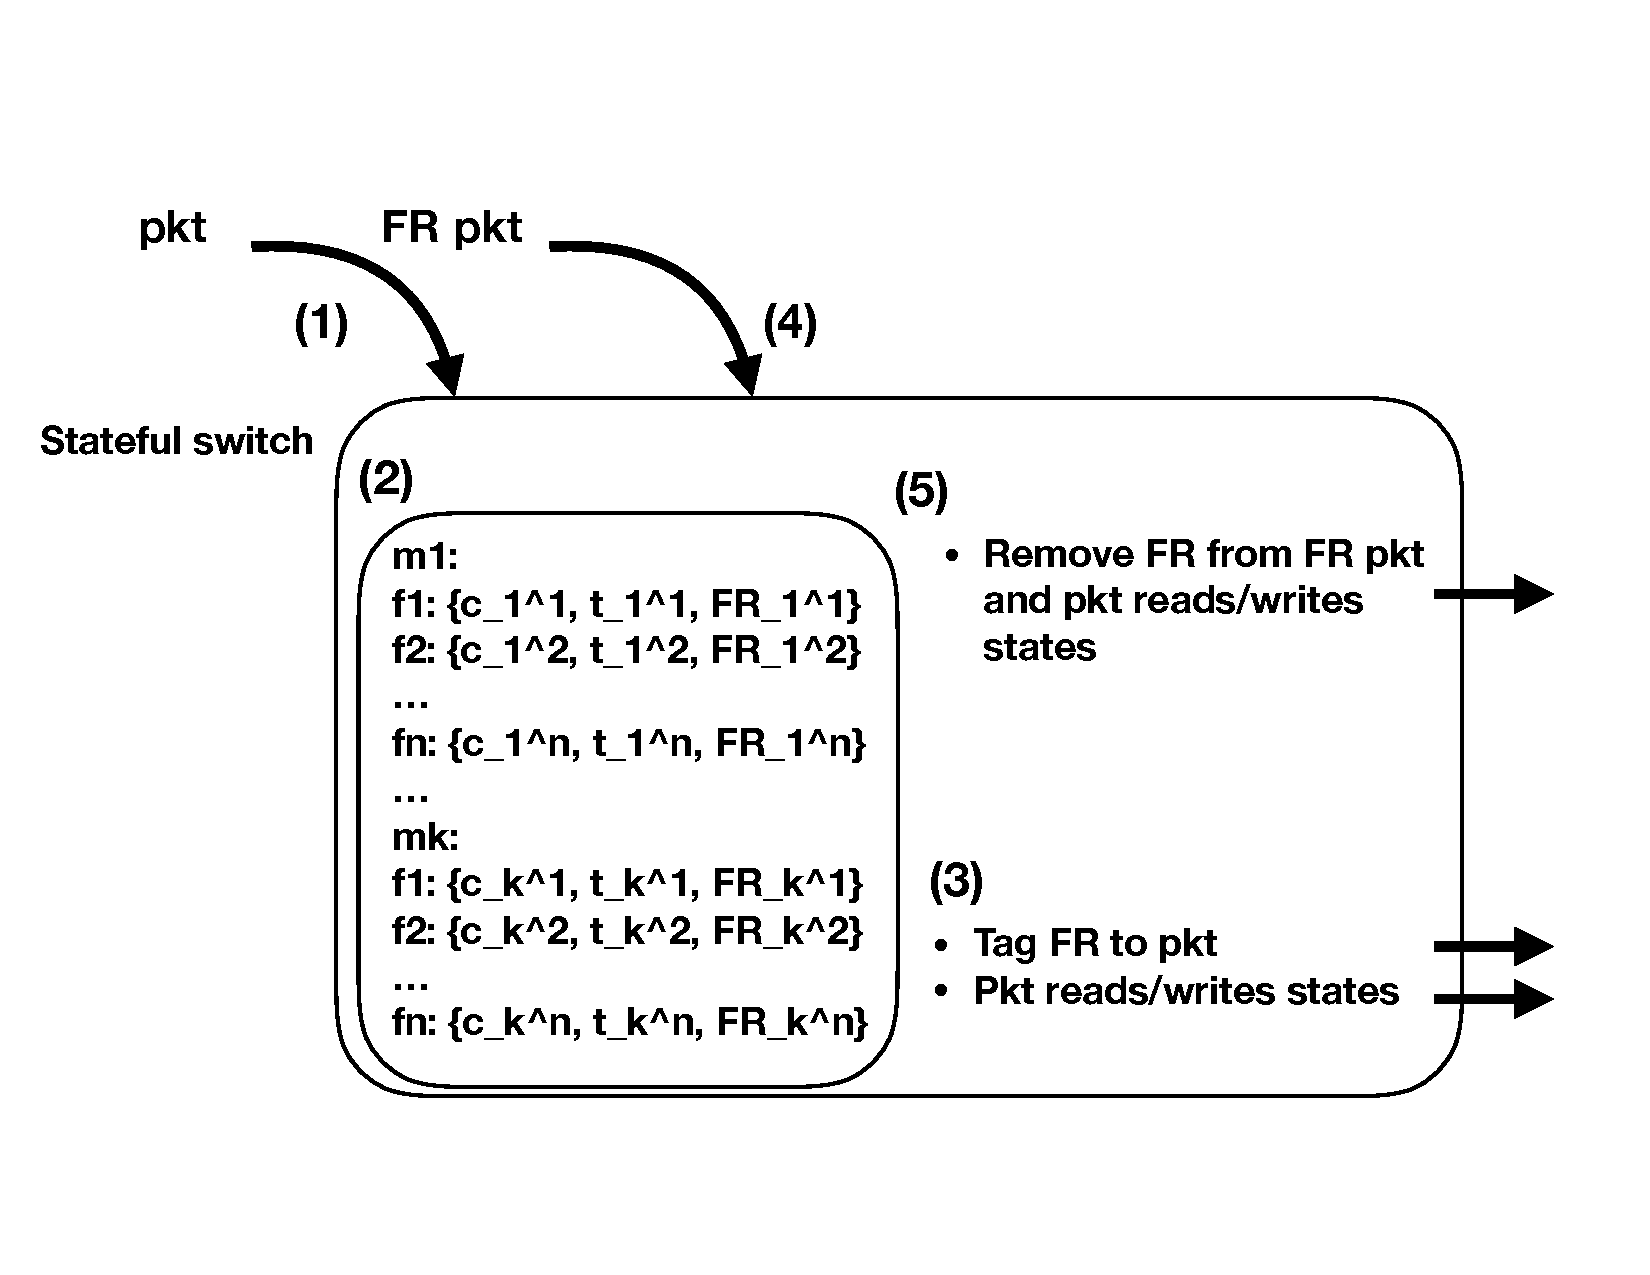
\includegraphics[width=\linewidth]{figures/71.pdf}
%\end{subfigure}
%%\vspace{-2mm}
%%\caption{\footnotesize{The CDF of job latency local and remote jobs.}}
%\caption{\small Workflow.}
%%\vspace{-2mm}
%\label{fig:mtv-example}
%\end{figure}
%
%
%

\section{Performance Evaluation}
\label{sec:eval}

%Dynamic Datapath Configuration (DDC)
In this section, we will first demonstrate the benefits of \concept{} from two aspects: latency and total throughput, and then give the evaluation for the waypoints constraints computation part. All evaluations are run on an 3.5 GHz Intel i7 processor with 16 GB of RAM running Mac OSX 10.13.

\para{Methodology}: First we generate a random topology with 25 nodes and 50 edges. For every edge, we set two random values as its latency (5 - 10 ms) and bandwidth (5 - 10 Mbps). To model a flow in the topology, we randomly choose two nodes from the topology as the source and destination nodes of the flow. And a flow can have a sequence of nodes (other than its source and destination nodes) in the topology as its required ordered middleboxes for packet processing. (We add a constraint to the selection for these middlebox nodes that the number of neighbors of a middlebox node must equal to two as typically a middlebox does not have route selection capability, \ie, for any packet, it only has one output interface.) As a comparison of \concept{}, the traditional approach does not distinguish whether a middlebox is stateful or stateless. Therefore, when computing a path for a flow in the tradition way (\ie, do not apply \concept{}), it requires the path must pass through all the middleboxes in a correct order. And when computing a path for a flow in the \concept{} approach, we random choose a subset of its required middlebox nodes as stateful middleboxes since for \concept{} approach, stateful and stateless middleboxes are handled in different ways.

\para{Latency}: To show the benefits for the latency aspect, we consider a single flow and differentiate its number of required middleboxes. And the target is to find the optimal path to minimize the latency for the flow. Then, we compare the results (\ie, the minimal latency) between applying \concept{} and not.

\para{Total throughput}: To show the benefits for the total throughput aspect, we consider multiple flows and all flows have the same required middleboxes. We also differentiate the number of middleboxes. And the target is to find optimal paths that have maximum total throughput. Then, we compare the results (\ie, the maximum total throughput) between applying \concept{} and not.

\para{Execution time}: To evaluate the performance of \concept{}, we compare the execution time of the path computation to maximize total throughput for both approaches (\ie, applying \concept{} and not).

\para{Waypoints constraints computation}: To show the benefits of the waypoints constraints computation, we set a sequence of nodes in the topology as a flow's waypoints constraint. Then, we consider the minimal latency as system's objective and compare the results between applying the waypoints constraints computation and not (\ie, leading to excessive constraints). In the excessive constraints, all the middlebox nodes should be passed through before flow's waypoints.



\para{Results}: The results in Fig.~\ref{fig:eval12}(a) demonstrate that by using \concept{}, the latency can be reduced. Specifically, $F$ specifies the number of flows; $M$ specifies the number of required middleboxes for flows; $S$ specifies the number of stateful middleboxes for flows. As minimizing latency for a flow does not affect the results of other flows, the experiment only considers one flow scenario. From the results, we can see that without \concept{}, the latency of the flow grows up when the number of stateless middleboxes increases but if \concept{} is applied, the latency grows up only when the number of stateful middleboxes increases.

The results in Fig.~\ref{fig:eval12}(b) demonstrate that by using \concept{}, the total throughput can be increased. Specifically, when there are 5 flows and 3 middleboxes, the total throughput with \concept{} is around 3 times compared with that without \concept{}.

\begin{figure}[!htbp]
%\vspace{-2mm}
\centering
\begin{subfigure}{0.48\linewidth}
      \centering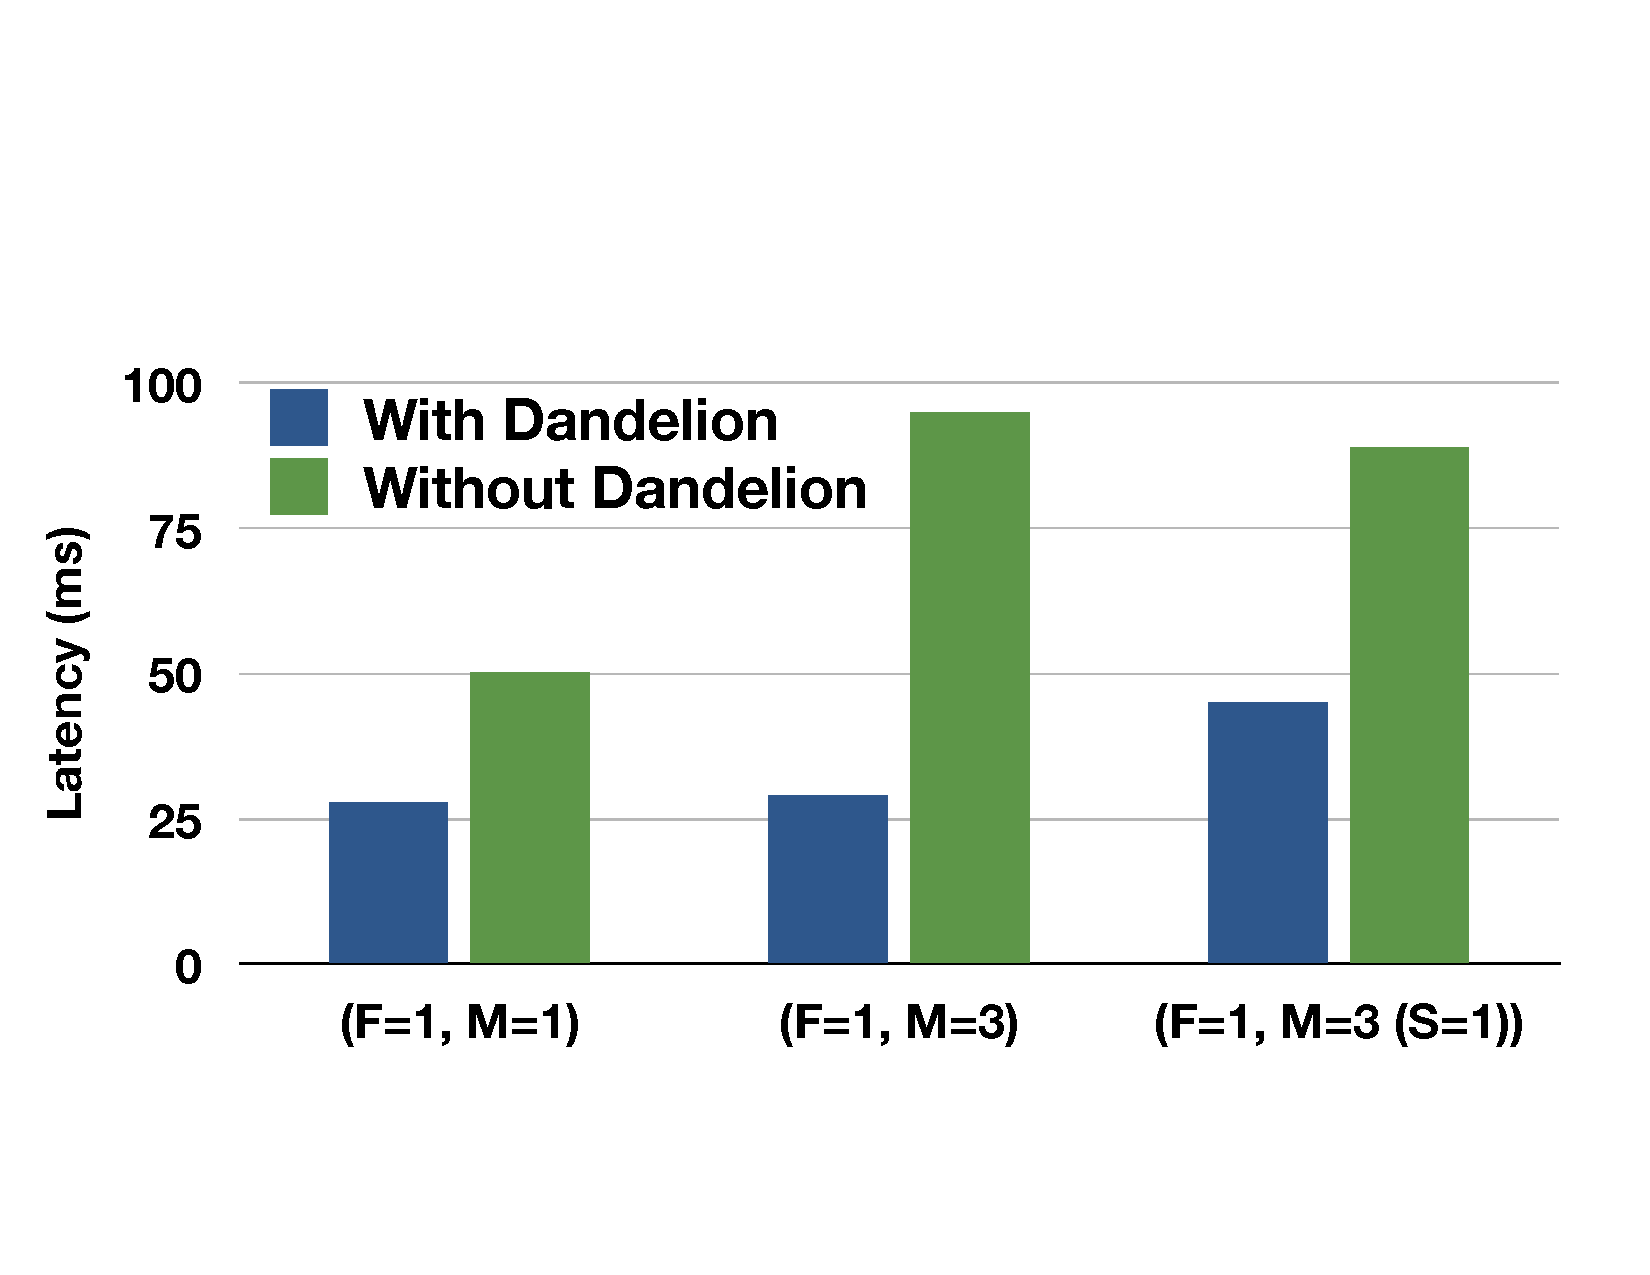
\includegraphics[width=\linewidth]{figures/ss-eval1.pdf}
      \caption{\label{fig:eval1} \small The latency for different scenarios.}
\end{subfigure}
%\hspace{0.03\linewidth}
\begin{subfigure}{0.48\linewidth}
      \centering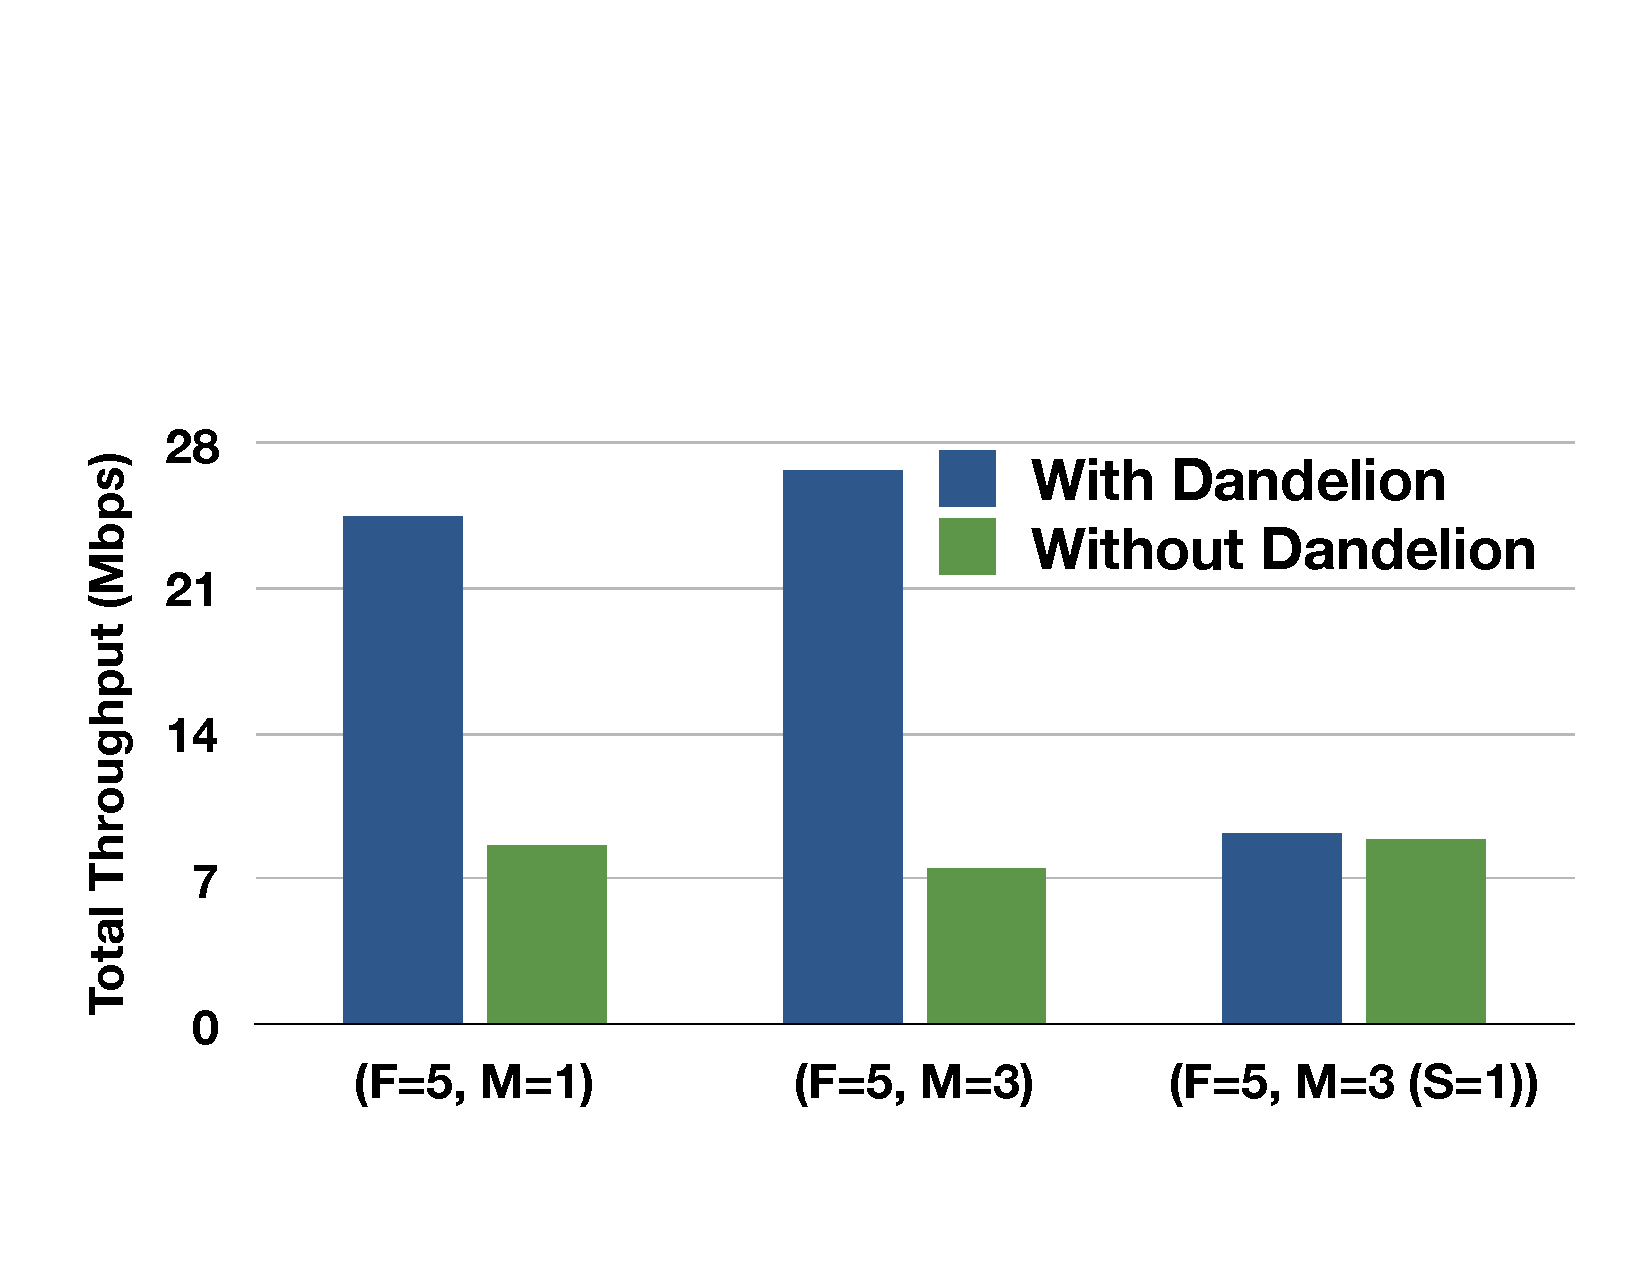
\includegraphics[width=\linewidth]{figures/ss-eval2.pdf}
      \caption{\label{fig:eval2} \small The total throughput for different scenarios.}
\end{subfigure}
\vspace{-2mm}
\caption{\small The benefits of \concept{} for latency and total throughput.}
%\vspace{-2mm}
\label{fig:eval12}
\end{figure}




%\begin{figure}[!htbp]
%%\vspace{-2mm}
%\centering
%\begin{subfigure}{0.8\linewidth}
%      \centering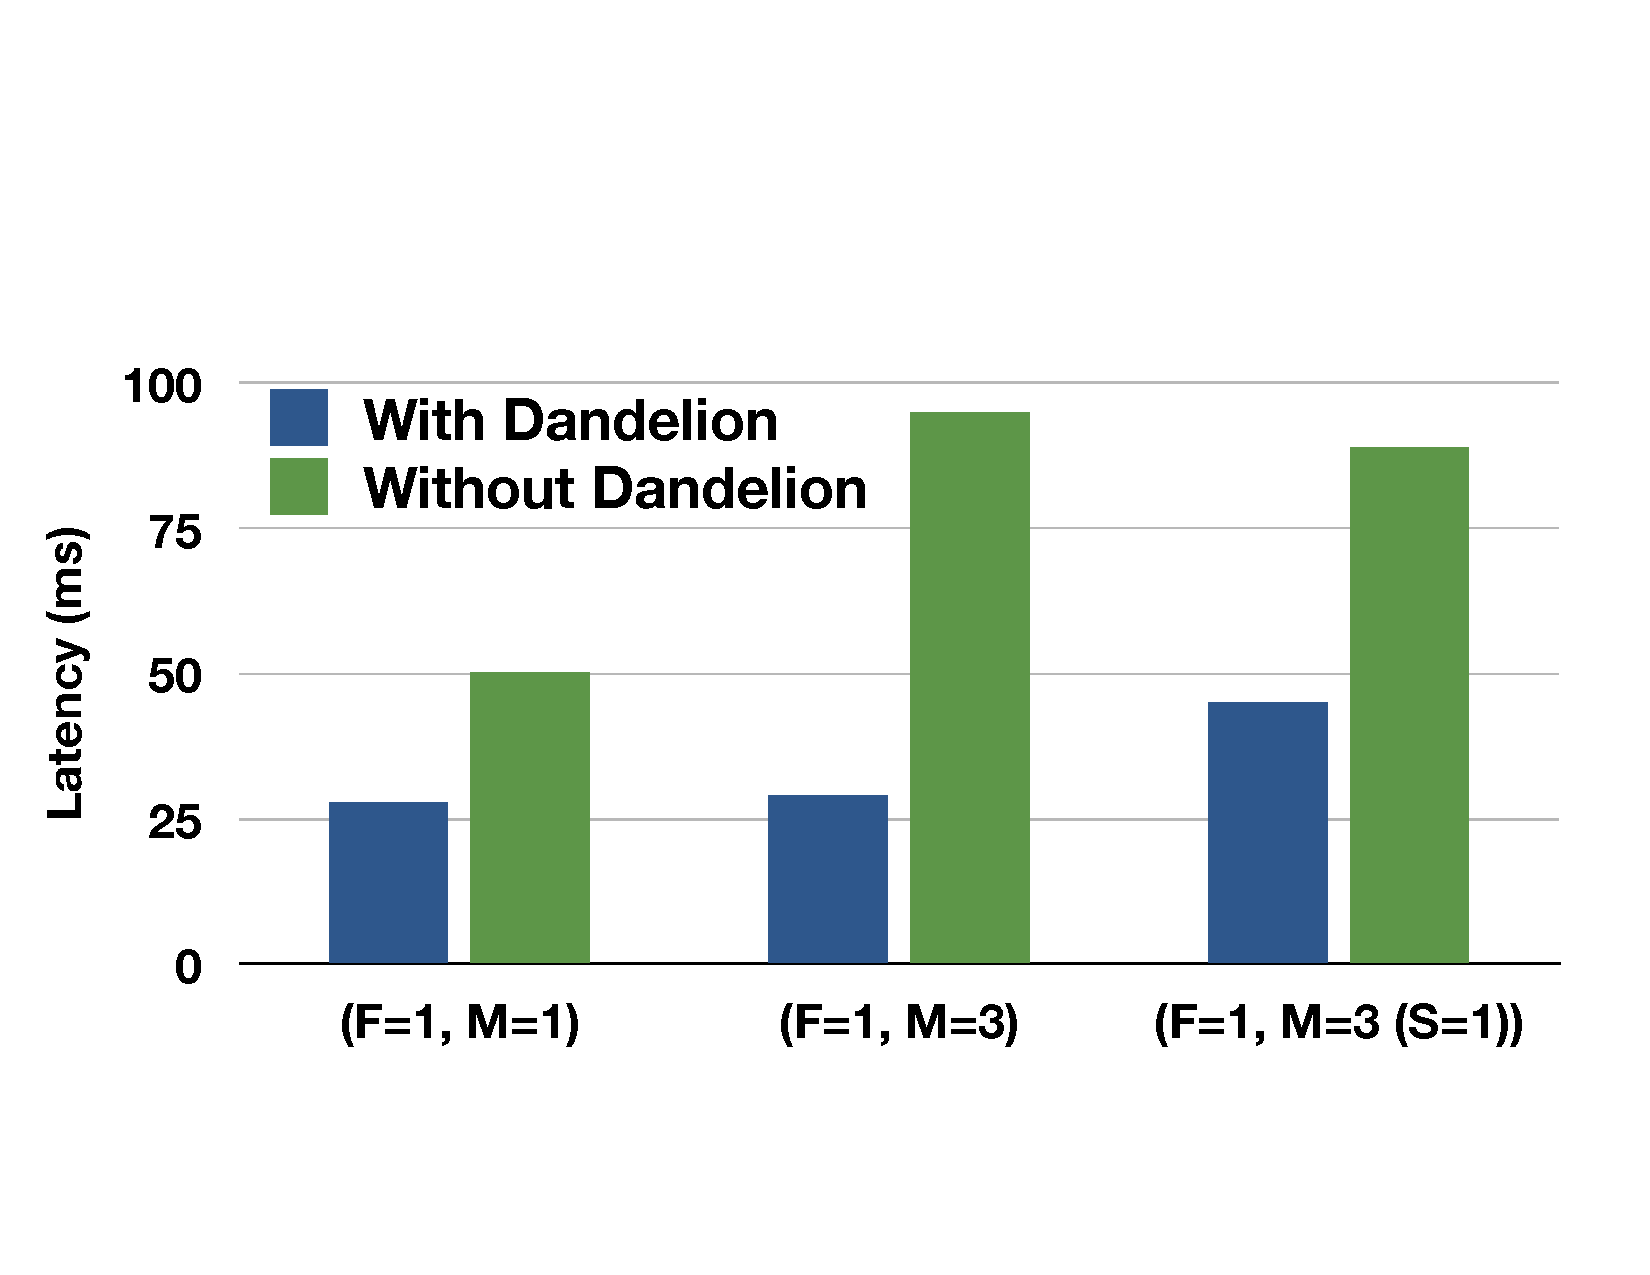
\includegraphics[width=\linewidth]{figures/ss-eval1.pdf}
%\end{subfigure}
%\hspace{0.03\linewidth}
%%\vspace{-2mm}
%%\caption{\footnotesize{The CDF of job latency local and remote jobs.}}
%\caption{\small The latency for different scenarios.}
%%\vspace{-2mm}
%\label{fig:eval1}
%\end{figure}




%\begin{figure}[!htbp]
%%\vspace{-2mm}
%\centering
%\begin{subfigure}{0.8\linewidth}
%      \centering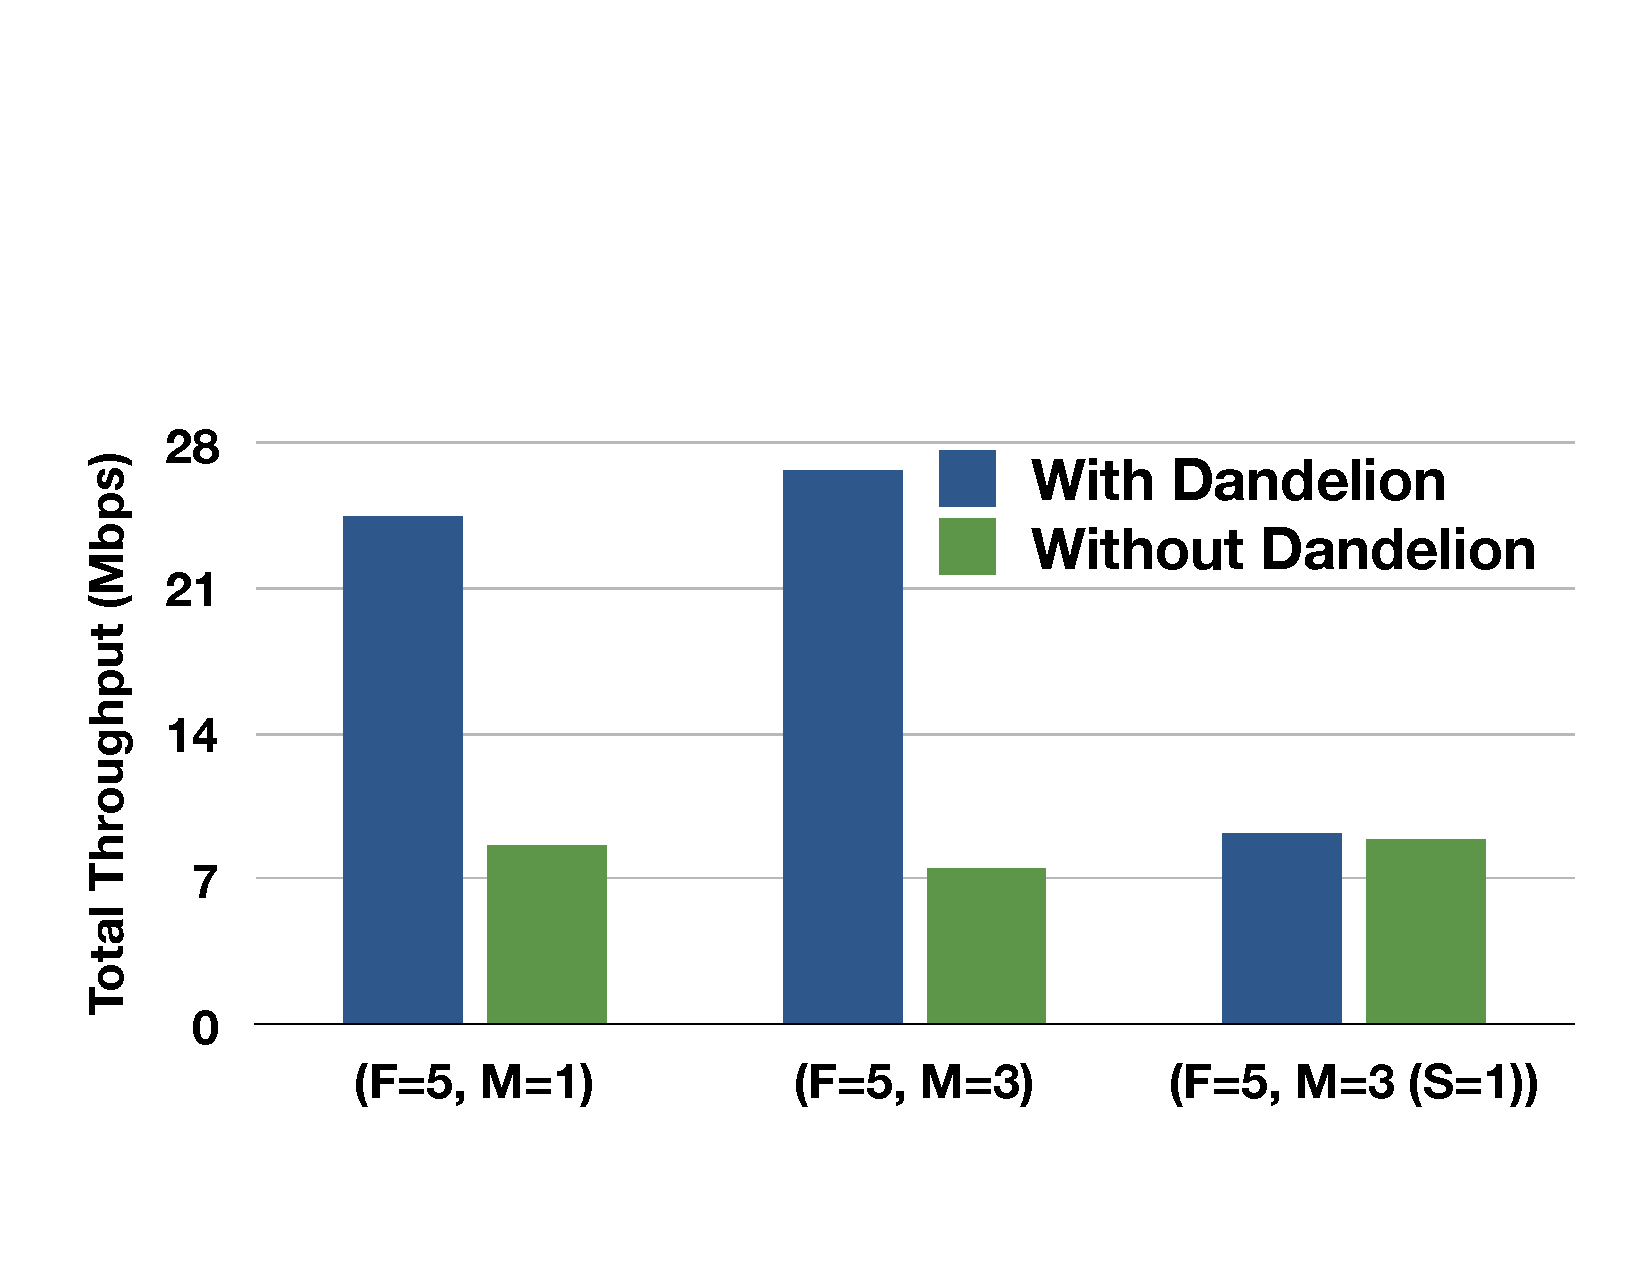
\includegraphics[width=\linewidth]{figures/ss-eval2.pdf}
%\end{subfigure}
%\hspace{0.03\linewidth}
%%\vspace{-2mm}
%%\caption{\footnotesize{The CDF of job latency local and remote jobs.}}
%\caption{\small The total throughput for different scenarios.}
%%\vspace{-2mm}
%\label{fig:eval2}
%\end{figure}

The results in Table~\ref{table:eval1} show the execution time of the path computation part to maximize total throughput. Since with \concept{}, the number of constraints is smaller than that without \concept{}, the execution time is also reduced (from 10.8 to 1.4 seconds when F=5 and M=3). 


\begin{table}[]
\footnotesize
\begin{tabular}{|l|l|l|l|}
\hline
             & \footnotesize(F=5, M=1) & \footnotesize (F=5, M=3) & \footnotesize (F=5, M=3 (S=1)) \\ \hline
With \concept{}    & 1.3 (s)    & 1.4 (s)    & 4.2 (s)          \\ \hline
Without \concept{} & 4.5 (s)    & 10.8 (s)   & 11.5 (s)         \\ \hline
\end{tabular}
\caption{\small The execution time of path computation to maximize total throughput for different scenarios.}
\label{table:eval1}
\end{table}


Fig.~\ref{fig:eval34} shows the latency with correct constraints (\ie, by
applying waypoints constraints computation) and with excessive constraints.
Specifically, the results in Fig.~\ref{fig:eval34}(a) consider that the
waypoints only have one node while Fig.~\ref{fig:eval34}(b) are for three nodes.
From the results, we can see the excessive constraints increase the latency,
\ie, lead to non-optimal path computation result. As the number of nodes
increases in the waypoints constraint, the latency with excessive constraints becomes larger.

\begin{figure}[!htbp]
%\vspace{-2mm}
\centering
\begin{subfigure}{0.48\linewidth}
      \centering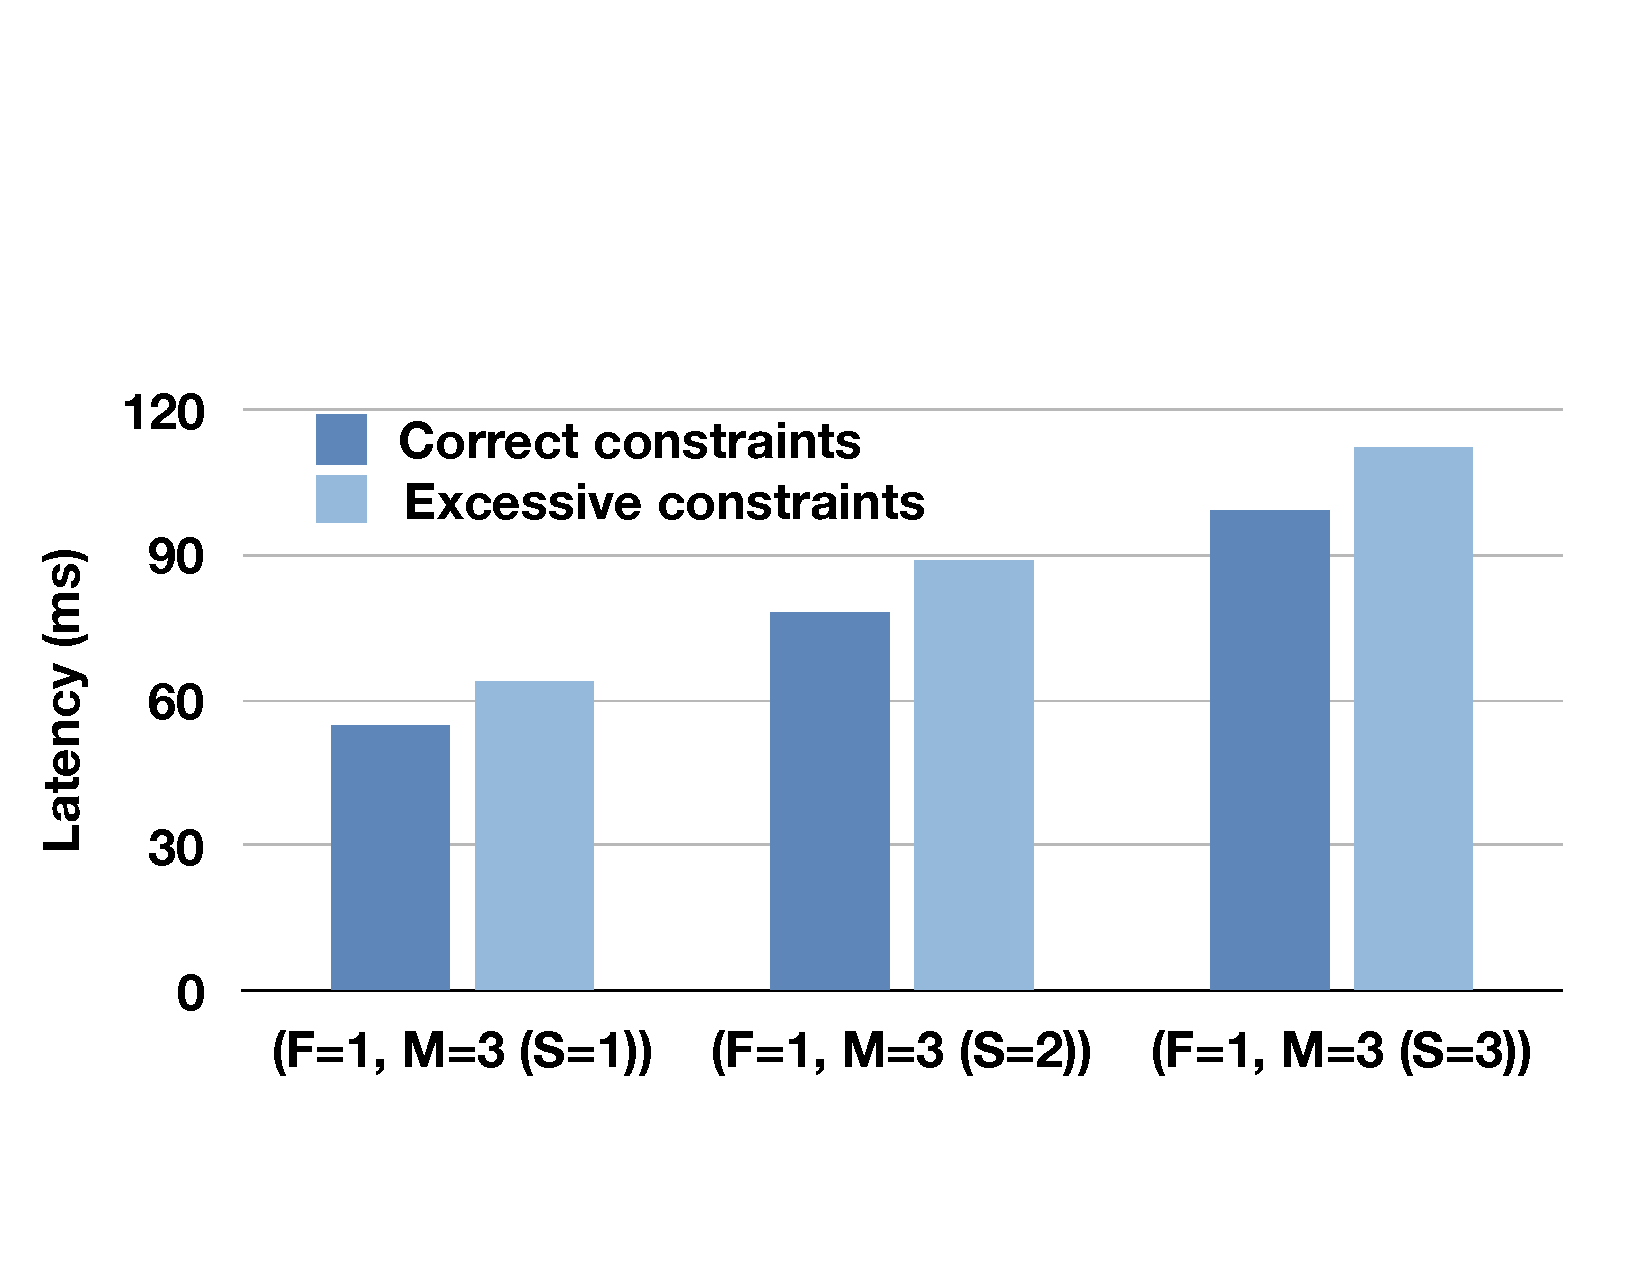
\includegraphics[width=\linewidth]{figures/ss-eval3.pdf}
      \caption{\label{fig:eval3} \small One node in waypoints constraint.}
\end{subfigure}
%\hspace{0.03\linewidth}
\begin{subfigure}{0.48\linewidth}
      \centering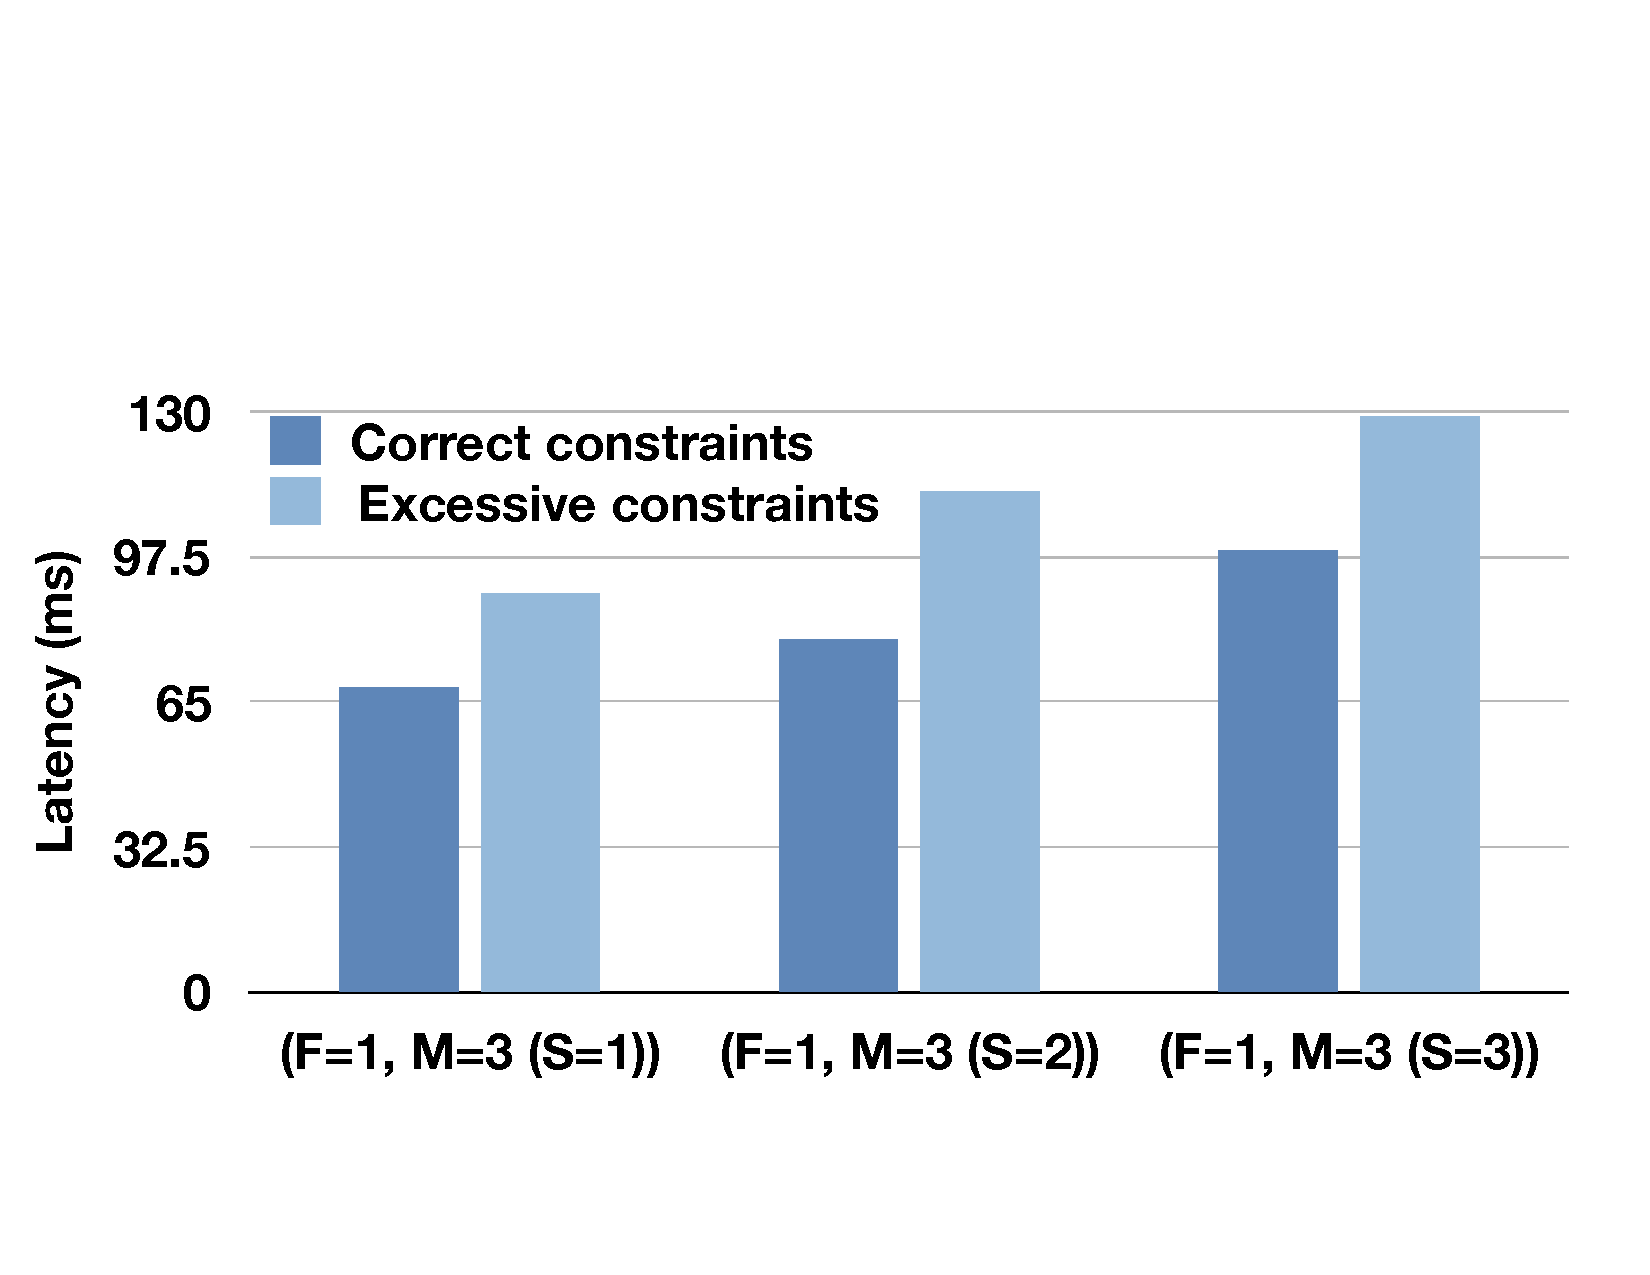
\includegraphics[width=\linewidth]{figures/ss-eval4.pdf}
      \caption{\label{fig:eval4} \small Three nodes in waypoints constraint.}
\end{subfigure}
\vspace{-2mm}
\caption{\small The latency with different waypoints constraints.}
%\vspace{-2mm}
\label{fig:eval34}
\end{figure}



%
%
%
%
%
%In this section, we will evaluate the proposed RSP design from two aspects: the execution time of pipeline design and the number of flow rules of the generated pipeline. All evaluations are run on an 3.5 GHz Intel i7 processor with 16 GB of RAM running Mac OSX 10.13.
%
%\subsection{Execution time}
%
%\para{Methodology}: Based on the analysis of the optimal pipeline design, we consider the following simple pipeline design algorithm: Given a DFG and $k$, recursively apply the source vertices selection $k-1$ times on the DFG to enumerates all the possible hardware pipelines. For the evaluation of both RSP and the unrolling approach, we randomly generate the DFG as the following: For the RSP, we change the number of software pipelines in the RSP (\ie, the number of iterations of the loop, $n$) and the number of vertices in the DFG of each pipeline (given the number of vertices, randomly generate the dataflow graph); For the unrolling approach, for each generated software pipeline in the RSP, we remove several vertices randomly. Then, we compare the execution time of RSP approach with the unrolling approach. Note that the complexity of enumerating all the possible pipelines equals to find the optimal pipeline as we do not consider the merging algorithm.
%
%%Then we evaluate the execution time of both RSP design and the unrolling approach. Specifically, for the evaluation of the RSP design, we change the number of software pipelines in the RSP and the number of vertices in the DFG of each pipeline (given the number of vertices, randomly generate the dataflow graph). To model the unrolling approach, for each pipeline in the repeated pipeline, we remove several vertices randomly. Then, we compare the execution time of repeated pipeline approach and the unrolling approach.
%
%\para{Result}: The result is shown in Figure~\ref{fig:eval1}. The horizontal axis specifies the number of iterations of the loop ($n$). The difference of Figure~\ref{fig:eval1-a} and Figure~\ref{fig:eval1-b} is the number of vertices ($m$) in the DFG of each software pipeline (for the unrolling approach, it means the number before removing vertices randomly) where $m = 10$ in Figure~\ref{fig:eval1-a} and $m = 20$ in Figure~\ref{fig:eval1-b}. And all the pipeline designs have the same $k$ as the limited number of flow tables where $k=10$. From the results, we can see that the RSP approach has smaller execution time compared (around 10 times when $n = 50$ and $m = 10$) with the unrolling approach when $k < n$. Note that when $n = 10$, both RSP and unrolling approach consider 10 software pipelines in the pipeline design, therefore, the execution time of both approaches is the same. And when $n = 100$, the execution time of unrolling is too large compared with the RSP approach.
%
%\begin{figure}[!htbp]
%%\vspace{-2mm}
%\centering
%\begin{subfigure}{0.47\linewidth}
%      \centering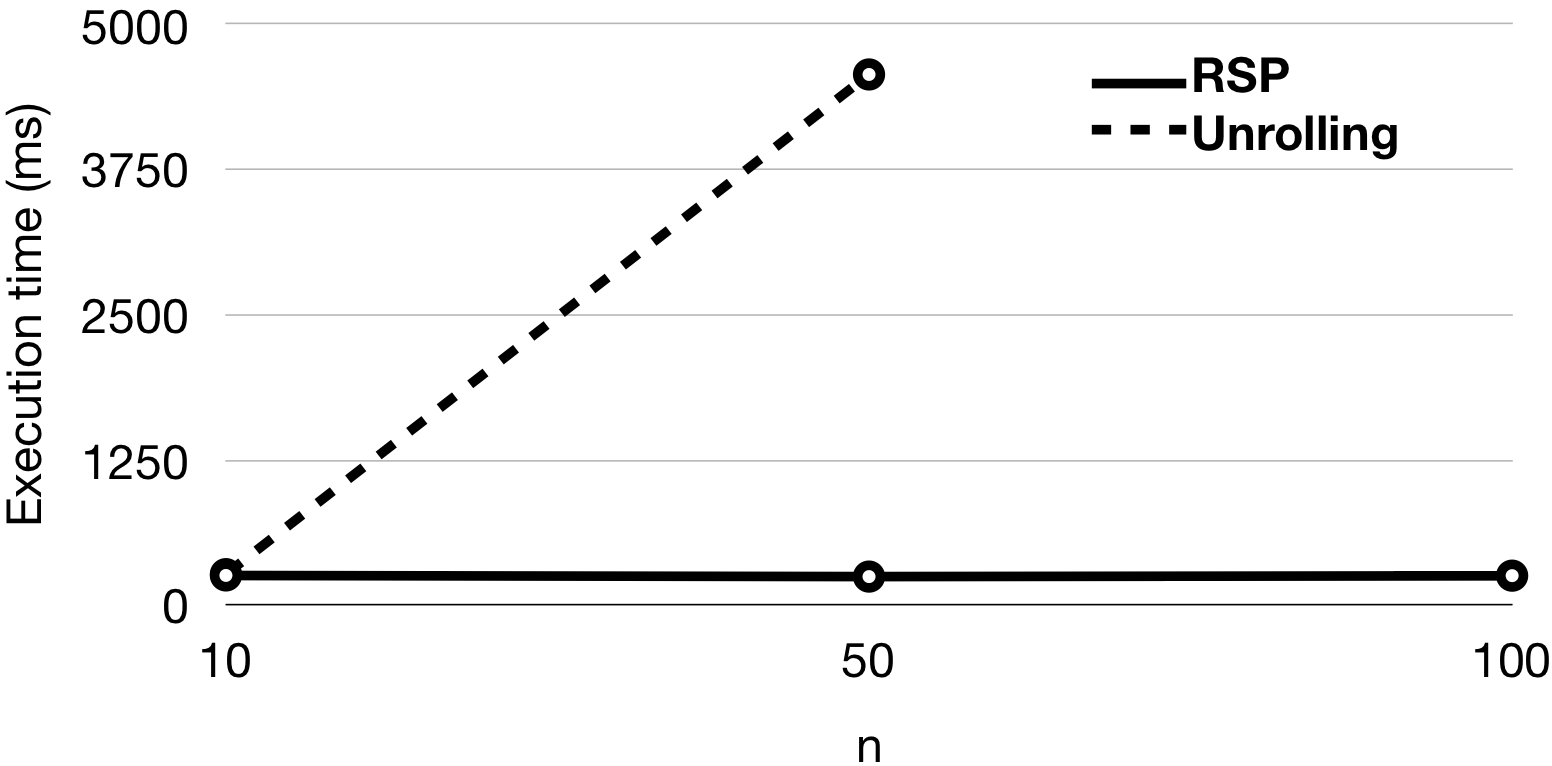
\includegraphics[width=\linewidth]{figures/lp-70.png}
%      \caption{\label{fig:eval1-a} \small $m$ = 10.}
%\end{subfigure}
%\hspace{0.03\linewidth}
%\begin{subfigure}{0.47\linewidth}
%      \centering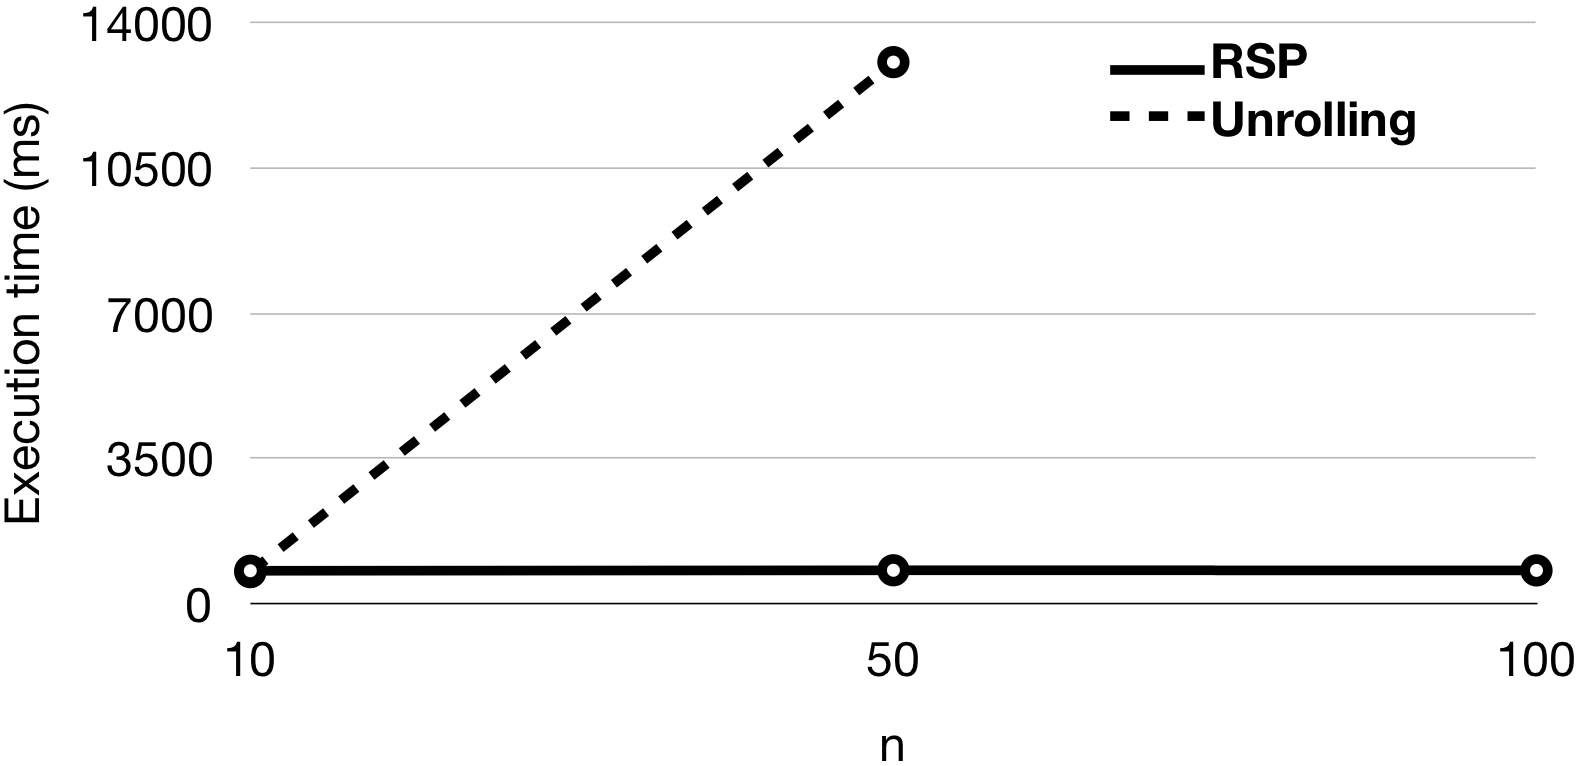
\includegraphics[width=\linewidth]{figures/lp-71.png}
%      \caption{\label{fig:eval1-b} \small $m$ = 20.}
%\end{subfigure}
%%\vspace{-2mm}
%%\caption{\footnotesize{The CDF of job latency local and remote jobs.}}
%\caption{\small The execution time of two approaches by changing the number of iterations ($n$) and the number of vertices ($m$).}
%%\vspace{-2mm}
%\label{fig:eval1}
%\end{figure}
%
%\subsection{Number of Flow Rules}
%
%\para{Methodology}: To compute the number of flow rules, we assign each variable (\ie, the vertex of DFG) the size of domain (\ie, the number of available values for the variable) randomly. Specifically, for the source vertices in the DFG of each software pipeline, we set the value from 100 to 200. And for the internal vertices in the DFG, we set the value from 10 to 20. This is because for the source vertices, they may represent packet fields which should have a larger range of values compared with internal variables in the program. Also, given a flow table, the computation of number of flow rules equals to the product of the size of domain of all the input variables. For example, a flow table consists of three input variables and their size of domain are 120, 10, 10 respectively, then the number of flow rules of the table is 12000. The definitions of $n$ and $m$ remain the same as the evaluation of execution time. We compare the number of flow rules of RSP design with the black-box approach (\ie, single table approach).
%
%\para{Result}: The result is shown in Table.~\ref{table:eval2}. As for the single table approach, the number of flow rules only depends on the first DFG of all software pipelines (which equals to the product of the size of domain of all the source vertices of the first DFG), so the values are the same for different $n$. From the result, we can find that the multi-table design can reduce the number of flow rules significantly compared with the single table approach. Also need to note that by the RSP approach, for each table, it may have a lot of unused flow rules. For example, the \codeword{while i in range(100)} statement can be viewed a flow table that matches \emph{i} and writes to \emph{i} with 100 flow rules (\ie, i = 0, 2, ..., 99), which has 99 unused flow rules when the table is the first table. Therefore, the number of flow rules can be reduced further by existing work which will not be discussed in this paper.
%
%\begin{table}[!htbp]
%\centering
%\begin{tabular}{|l|l|l|}
%\hline
%         & n =10, m = 10 & n = 50, m= 10 \\ \hline
%Single  & 3898434       & 3898434       \\ \hline
%RSP & 61856         & 224098        \\ \hline
%\end{tabular}
%\caption{\small The number of flow rules of the single table approach and the RSP approach.}
%\label{table:eval2}
%\end{table}
%


%\section{Related Work}\label{sec:related-work}
\para{High level SDN Program Compilers:} Multiple systems that allow programmers to write SDN programs in high level languages and then compile such programs to flow table pipelines have been proposed over the last several years. Such systems are related to our work in that they examine the transformation of policy programs into switch flow tables. We group these systems into two categories: \textit{tier-less} and \textit{split-level}.

\textit{Tier-less} systems (\eg\ SNAP~\cite{SNAP}, FML~\cite{fml}, FlowLog~\cite{flowlog},  Maple~\cite{maple}), require programmers to specify forwarding behaviors as packet handling functions which are then used by the SDN controller to configure and update network state. Such systems pioneer our pipeline capacity theorem's notion of a \textit{program function} and are able to compile such functions to single pipelines. These systems, however, are unable to verify that submitted functions can be written to a given pipeline without physically carrying out the time consuming process of compilation, and cannot write programs to multi-pipeline networks.

\textit{Split-level} systems such as the Frentic family (\eg\ Frenetic~\cite{frenetic}, Pyretic~\cite{pyretic}) provide a two tiered programming model in which controller programs specify events of interest and then respond to these events when they occur by calculating new network policies. Again, such systems cannot verify that a given controller program's output can be written to the controller's switches' pipelines, although this paradigm falls outside of our pipeline capacity theorem's model as well.

\para{Pipeline specification languages:} There are some superficial similarities between pipeline specification languages (\eg\ P4~\cite{P4}, PISCES~\cite{PISCES}, Concurrent NetCore~\cite{ConcurrentNetCore}) and our pipeline capacity theorem, such as the analysis and guarantees that such languages provide about pipeline behavior. For example, Concurrent NetCore's type system ensures that any program used to populate a pipeline has certain properties, such as determinism, whilst PISCES's switch specification allows compilers to analyze pipelines and optimize their performance. We contend, however, that our capacity theorem attacks an entirely different space in pipeline analysis - guaranteeing pipeline properties or improving performance is qualitatively different to verifying whether compilation is possible.

%\para{Multi-switch network programming:} Our pipeline capacity algebra is related to other systems that facilitate multi-switch network programming, specifically DIFANE~\cite{DIFANE} and TableVisor~\cite{TableVisor}. These systems, however, focus on distributing a centrally specified flow table/flow table pipeline across a given network, whilst our algebra verifies that generic high level language programs can be written to it.

\para{Pipeline design:} Pipeline design schemes such as Jose et al.'s ``Compiling Packet Programs to Reconfigurable Switches''~\cite{Jose-et-al}, Sun et al.'s ``Software-Defined Flow Table Pipeline''~\cite{Sun-et-al}, FlowAdapter~\cite{FlowAdapter}, and Domino~\cite{Domino} are clearly related to our pipeline capacity theorem in that they examine pipeline layout design under hardware constraints. Jose et al., Sun et al., and FlowAdapter  however, focus on mapping logical lookup tables/flow table pipelines to physical tables whilst our pipeline capacity theorem focuses on generic programs, while Domino considers weaker hardware constraints (\eg\ limits on stateful operations at line-rate) than our work does.

\vspace{-2mm}
\section{Conclusion}\label{sec:conclusion}
\vspace{-1mm}
We design \concept{}, a novel, high-level SDC programming system providing novel high-level primitives for users to specify the behavior
	of SDC data plane devices, and automatically translates
high-level SDC programs into efficient SDC datapath configurations with local
state sharing. Experiment results demonstrate its efficiency and efficacy.
\vspace{-4mm}







\bibliographystyle{IEEEtran}
\bibliography{all}

%\begin{abstract}
%This document is a model and instructions for \LaTeX.
%This and the IEEEtran.cls file define the components of your paper [title, text, heads, etc.]. *CRITICAL: Do Not Use Symbols, Special Characters, Footnotes, 
%or Math in Paper Title or Abstract.
%\end{abstract}
%
%\begin{IEEEkeywords}
%component, formatting, style, styling, insert
%\end{IEEEkeywords}
%
%\section{Introduction}
%This document is a model and instructions for \LaTeX.
%Please observe the conference page limits. 
%
%\section{Ease of Use}
%
%\subsection{Maintaining the Integrity of the Specifications}
%
%The IEEEtran class file is used to format your paper and style the text. All margins, 
%column widths, line spaces, and text fonts are prescribed; please do not 
%alter them. You may note peculiarities. For example, the head margin
%measures proportionately more than is customary. This measurement 
%and others are deliberate, using specifications that anticipate your paper 
%as one part of the entire proceedings, and not as an independent document. 
%Please do not revise any of the current designations.
%
%\section{Prepare Your Paper Before Styling}
%Before you begin to format your paper, first write and save the content as a 
%separate text file. Complete all content and organizational editing before 
%formatting. Please note sections \ref{AA}--\ref{SCM} below for more information on 
%proofreading, spelling and grammar.
%
%Keep your text and graphic files separate until after the text has been 
%formatted and styled. Do not number text heads---{\LaTeX} will do that 
%for you.
%
%\subsection{Abbreviations and Acronyms}\label{AA}
%Define abbreviations and acronyms the first time they are used in the text, 
%even after they have been defined in the abstract. Abbreviations such as 
%IEEE, SI, MKS, CGS, ac, dc, and rms do not have to be defined. Do not use 
%abbreviations in the title or heads unless they are unavoidable.
%
%\subsection{Units}
%\begin{itemize}
%\item Use either SI (MKS) or CGS as primary units. (SI units are encouraged.) English units may be used as secondary units (in parentheses). An exception would be the use of English units as identifiers in trade, such as ``3.5-inch disk drive''.
%\item Avoid combining SI and CGS units, such as current in amperes and magnetic field in oersteds. This often leads to confusion because equations do not balance dimensionally. If you must use mixed units, clearly state the units for each quantity that you use in an equation.
%\item Do not mix complete spellings and abbreviations of units: ``Wb/m\textsuperscript{2}'' or ``webers per square meter'', not ``webers/m\textsuperscript{2}''. Spell out units when they appear in text: ``. . . a few henries'', not ``. . . a few H''.
%\item Use a zero before decimal points: ``0.25'', not ``.25''. Use ``cm\textsuperscript{3}'', not ``cc''.)
%\end{itemize}
%
%\subsection{Equations}
%Number equations consecutively. To make your 
%equations more compact, you may use the solidus (~/~), the exp function, or 
%appropriate exponents. Italicize Roman symbols for quantities and variables, 
%but not Greek symbols. Use a long dash rather than a hyphen for a minus 
%sign. Punctuate equations with commas or periods when they are part of a 
%sentence, as in:
%\begin{equation}
%a+b=\gamma\label{eq}
%\end{equation}
%
%Be sure that the 
%symbols in your equation have been defined before or immediately following 
%the equation. Use ``\eqref{eq}'', not ``Eq.~\eqref{eq}'' or ``equation \eqref{eq}'', except at 
%the beginning of a sentence: ``Equation \eqref{eq} is . . .''
%
%\subsection{\LaTeX-Specific Advice}
%
%Please use ``soft'' (e.g., \verb|\eqref{Eq}|) cross references instead
%of ``hard'' references (e.g., \verb|(1)|). That will make it possible
%to combine sections, add equations, or change the order of figures or
%citations without having to go through the file line by line.
%
%Please don't use the \verb|{eqnarray}| equation environment. Use
%\verb|{align}| or \verb|{IEEEeqnarray}| instead. The \verb|{eqnarray}|
%environment leaves unsightly spaces around relation symbols.
%
%Please note that the \verb|{subequations}| environment in {\LaTeX}
%will increment the main equation counter even when there are no
%equation numbers displayed. If you forget that, you might write an
%article in which the equation numbers skip from (17) to (20), causing
%the copy editors to wonder if you've discovered a new method of
%counting.
%
%{\BibTeX} does not work by magic. It doesn't get the bibliographic
%data from thin air but from .bib files. If you use {\BibTeX} to produce a
%bibliography you must send the .bib files. 
%
%{\LaTeX} can't read your mind. If you assign the same label to a
%subsubsection and a table, you might find that Table I has been cross
%referenced as Table IV-B3. 
%
%{\LaTeX} does not have precognitive abilities. If you put a
%\verb|\label| command before the command that updates the counter it's
%supposed to be using, the label will pick up the last counter to be
%cross referenced instead. In particular, a \verb|\label| command
%should not go before the caption of a figure or a table.
%
%Do not use \verb|\nonumber| inside the \verb|{array}| environment. It
%will not stop equation numbers inside \verb|{array}| (there won't be
%any anyway) and it might stop a wanted equation number in the
%surrounding equation.
%
%\subsection{Some Common Mistakes}\label{SCM}
%\begin{itemize}
%\item The word ``data'' is plural, not singular.
%\item The subscript for the permeability of vacuum $\mu_{0}$, and other common scientific constants, is zero with subscript formatting, not a lowercase letter ``o''.
%\item In American English, commas, semicolons, periods, question and exclamation marks are located within quotation marks only when a complete thought or name is cited, such as a title or full quotation. When quotation marks are used, instead of a bold or italic typeface, to highlight a word or phrase, punctuation should appear outside of the quotation marks. A parenthetical phrase or statement at the end of a sentence is punctuated outside of the closing parenthesis (like this). (A parenthetical sentence is punctuated within the parentheses.)
%\item A graph within a graph is an ``inset'', not an ``insert''. The word alternatively is preferred to the word ``alternately'' (unless you really mean something that alternates).
%\item Do not use the word ``essentially'' to mean ``approximately'' or ``effectively''.
%\item In your paper title, if the words ``that uses'' can accurately replace the word ``using'', capitalize the ``u''; if not, keep using lower-cased.
%\item Be aware of the different meanings of the homophones ``affect'' and ``effect'', ``complement'' and ``compliment'', ``discreet'' and ``discrete'', ``principal'' and ``principle''.
%\item Do not confuse ``imply'' and ``infer''.
%\item The prefix ``non'' is not a word; it should be joined to the word it modifies, usually without a hyphen.
%\item There is no period after the ``et'' in the Latin abbreviation ``et al.''.
%\item The abbreviation ``i.e.'' means ``that is'', and the abbreviation ``e.g.'' means ``for example''.
%\end{itemize}
%An excellent style manual for science writers is \cite{b7}.
%
%\subsection{Authors and Affiliations}
%\textbf{The class file is designed for, but not limited to, six authors.} A 
%minimum of one author is required for all conference articles. Author names 
%should be listed starting from left to right and then moving down to the 
%next line. This is the author sequence that will be used in future citations 
%and by indexing services. Names should not be listed in columns nor group by 
%affiliation. Please keep your affiliations as succinct as possible (for 
%example, do not differentiate among departments of the same organization).
%
%\subsection{Identify the Headings}
%Headings, or heads, are organizational devices that guide the reader through 
%your paper. There are two types: component heads and text heads.
%
%Component heads identify the different components of your paper and are not 
%topically subordinate to each other. Examples include Acknowledgments and 
%References and, for these, the correct style to use is ``Heading 5''. Use 
%``figure caption'' for your Figure captions, and ``table head'' for your 
%table title. Run-in heads, such as ``Abstract'', will require you to apply a 
%style (in this case, italic) in addition to the style provided by the drop 
%down menu to differentiate the head from the text.
%
%Text heads organize the topics on a relational, hierarchical basis. For 
%example, the paper title is the primary text head because all subsequent 
%material relates and elaborates on this one topic. If there are two or more 
%sub-topics, the next level head (uppercase Roman numerals) should be used 
%and, conversely, if there are not at least two sub-topics, then no subheads 
%should be introduced.
%
%\subsection{Figures and Tables}
%\paragraph{Positioning Figures and Tables} Place figures and tables at the top and 
%bottom of columns. Avoid placing them in the middle of columns. Large 
%figures and tables may span across both columns. Figure captions should be 
%below the figures; table heads should appear above the tables. Insert 
%figures and tables after they are cited in the text. Use the abbreviation 
%``Fig.~\ref{fig}'', even at the beginning of a sentence.
%
%\begin{table}[htbp]
%\caption{Table Type Styles}
%\begin{center}
%\begin{tabular}{|c|c|c|c|}
%\hline
%\textbf{Table}&\multicolumn{3}{|c|}{\textbf{Table Column Head}} \\
%\cline{2-4} 
%\textbf{Head} & \textbf{\textit{Table column subhead}}& \textbf{\textit{Subhead}}& \textbf{\textit{Subhead}} \\
%\hline
%copy& More table copy$^{\mathrm{a}}$& &  \\
%\hline
%\multicolumn{4}{l}{$^{\mathrm{a}}$Sample of a Table footnote.}
%\end{tabular}
%\label{tab1}
%\end{center}
%\end{table}
%
%\begin{figure}[htbp]
%\centerline{\includegraphics{fig1.png}}
%\caption{Example of a figure caption.}
%\label{fig}
%\end{figure}
%
%Figure Labels: Use 8 point Times New Roman for Figure labels. Use words 
%rather than symbols or abbreviations when writing Figure axis labels to 
%avoid confusing the reader. As an example, write the quantity 
%``Magnetization'', or ``Magnetization, M'', not just ``M''. If including 
%units in the label, present them within parentheses. Do not label axes only 
%with units. In the example, write ``Magnetization (A/m)'' or ``Magnetization 
%\{A[m(1)]\}'', not just ``A/m''. Do not label axes with a ratio of 
%quantities and units. For example, write ``Temperature (K)'', not 
%``Temperature/K''.
%
%\section*{Acknowledgment}
%
%The preferred spelling of the word ``acknowledgment'' in America is without 
%an ``e'' after the ``g''. Avoid the stilted expression ``one of us (R. B. 
%G.) thanks $\ldots$''. Instead, try ``R. B. G. thanks$\ldots$''. Put sponsor 
%acknowledgments in the unnumbered footnote on the first page.
%
%\section*{References}
%
%Please number citations consecutively within brackets \cite{b1}. The 
%sentence punctuation follows the bracket \cite{b2}. Refer simply to the reference 
%number, as in \cite{b3}---do not use ``Ref. \cite{b3}'' or ``reference \cite{b3}'' except at 
%the beginning of a sentence: ``Reference \cite{b3} was the first $\ldots$''
%
%Number footnotes separately in superscripts. Place the actual footnote at 
%the bottom of the column in which it was cited. Do not put footnotes in the 
%abstract or reference list. Use letters for table footnotes.
%
%Unless there are six authors or more give all authors' names; do not use 
%``et al.''. Papers that have not been published, even if they have been 
%submitted for publication, should be cited as ``unpublished'' \cite{b4}. Papers 
%that have been accepted for publication should be cited as ``in press'' \cite{b5}. 
%Capitalize only the first word in a paper title, except for proper nouns and 
%element symbols.
%
%For papers published in translation journals, please give the English 
%citation first, followed by the original foreign-language citation \cite{b6}.
%
%\begin{thebibliography}{00}
%\bibitem{b1} G. Eason, B. Noble, and I. N. Sneddon, ``On certain integrals of Lipschitz-Hankel type involving products of Bessel functions,'' Phil. Trans. Roy. Soc. London, vol. A247, pp. 529--551, April 1955.
%\bibitem{b2} J. Clerk Maxwell, A Treatise on Electricity and Magnetism, 3rd ed., vol. 2. Oxford: Clarendon, 1892, pp.68--73.
%\bibitem{b3} I. S. Jacobs and C. P. Bean, ``Fine particles, thin films and exchange anisotropy,'' in Magnetism, vol. III, G. T. Rado and H. Suhl, Eds. New York: Academic, 1963, pp. 271--350.
%\bibitem{b4} K. Elissa, ``Title of paper if known,'' unpublished.
%\bibitem{b5} R. Nicole, ``Title of paper with only first word capitalized,'' J. Name Stand. Abbrev., in press.
%\bibitem{b6} Y. Yorozu, M. Hirano, K. Oka, and Y. Tagawa, ``Electron spectroscopy studies on magneto-optical media and plastic substrate interface,'' IEEE Transl. J. Magn. Japan, vol. 2, pp. 740--741, August 1987 [Digests 9th Annual Conf. Magnetics Japan, p. 301, 1982].
%\bibitem{b7} M. Young, The Technical Writer's Handbook. Mill Valley, CA: University Science, 1989.
%\end{thebibliography}
%\vspace{12pt}
%\color{red}
%IEEE conference templates contain guidance text for composing and formatting conference papers. Please ensure that all template text is removed from your conference paper prior to submission to the conference. Failure to remove the template text from your paper may result in your paper not being published.
%
\end{document}
